\documentclass[a4paper]{book}
\usepackage{a4wide}
\usepackage{makeidx}
\usepackage{fancyhdr}
\usepackage{graphicx}
\usepackage{multicol}
\usepackage{color}
\usepackage{float}
\usepackage{textcomp}
\usepackage{alltt}
\usepackage{doxygen}
\makeindex
\setcounter{tocdepth}{1}
\renewcommand{\footrulewidth}{0.4pt}

%-------------------------
% begin and end equations
%-------------------------
\newcommand{\be} {\begin{equation}}
\newcommand{\ee} {\end{equation}}
\newcommand{\bea}{\begin{eqnarray}}
\newcommand{\eea}{\end{eqnarray}}
\newcommand{\ba} {\begin{array}}
\newcommand{\ea} {\end{array}}

%-----------------
% text formatting 
%-----------------
\newcommand{\noi}{\noindent}

%---------------
% special signs
%---------------
\newcommand{\p}  {\partial}
\newcommand{\s}  {\star}
\newcommand{\Dx} {\Delta}

%-----------------
% velocity vector
%-----------------
\newcommand{\uvw}{{\bf u}}          

%---------------------------
% putting things up or down
%---------------------------
\newcommand{\ol} {\overline}
\newcommand{\ul} {\underline}

%---------------------
% logical coordinates
%---------------------
\newcommand{\ijk}     { {i,j,k} }      % central

\newcommand{\ipjk}    { {i+1,j,k} }    % i+1
\newcommand{\imjk}    { {i-1,j,k} }    % i-1
\newcommand{\ijpk}    { {i,j+1,k} }    % j+1
\newcommand{\ijmk}    { {i,j-1,k} }    % j-1
\newcommand{\ijkp}    { {i,j,k+1} }    % k+1
\newcommand{\ijkm}    { {i,j,k-1} }    % k-1

\newcommand{\ijpkp}   { {i,j+1,k+1} }  % i
\newcommand{\ijpkm}   { {i,j+1,k-1} }
\newcommand{\ijmkp}   { {i,j-1,k+1} }
\newcommand{\ijmkm}   { {i,j-1,k-1} }

\newcommand{\ipjkp}   { {i+1,j,k+1} }  % j
\newcommand{\ipjkm}   { {i+1,j,k-1} }
\newcommand{\imjkp}   { {i-1,j,k+1} }
\newcommand{\imjkm}   { {i-1,j,k-1} }

\newcommand{\ipjpk}   { {i+1,j+1,k} }  % k
\newcommand{\ipjmk}   { {i+1,j-1,k} }
\newcommand{\imjpk}   { {i-1,j+1,k} }
\newcommand{\imjmk}   { {i-1,j-1,k} }

%--------------------------------------
% compute length for framing equations
%--------------------------------------
\newlength{\ii}
\setlength{\ii}{\textwidth}
\addtolength{\ii}{-2\fboxsep}
\addtolength{\ii}{-2\fboxrule}

% To frame an equation, use:
% \begin{center} \fbox{ \begin{minipage}{\ii} \be
% ... equation ... 
% \ee \end{minipage} } \end{center}

%-------------------
% to include figures
%-------------------
\usepackage{graphicx}
\usepackage{psfrag}
% \newcommand{\thickbox}[2]{\thicklines\put(0,0){\framebox(#1,#2){}}}
\newcommand{\thickbox}[2]{}

%----------------------------
% fancy mathematical symbols
%----------------------------
\usepackage{amssymb}

%---------------
% PSI-Boil sign
%---------------
\newcommand{\psiboil}{\sffamily PSI-Boil}


\definecolor{darkblue}{rgb}{0.0, 0.0, 0.5}

\begin{document}

  %--------------%
  %              %
  %  Title Page  %
  %              %
  %--------------%
  \title{ {\Huge {\bfseries\psiboil} {\bf Tutorial}} \\
           \vspace{10mm}
          {\huge {\bf Volume 1: Fundamentals} } }

  \author{{\Large Bojan Ni\v{c}eno}                     \\
          {\em Laboratory for Simulation Modelling and Computation} \\
          {\em Paul Scherrer Institut, 5232 Villigen PSI, Switzerland}  \\
          {\tt bojan.niceno@psi.ch} \\ \\
          {\em updated by} {\Large Yohei Sato} \\
          {\tt yohei.sato@psi.ch}}

  \maketitle

  \clearemptydoublepage

  \pagenumbering{roman}

  %---------------------%
  %                     %
  %  Table of Contents  %
  %                     %
  %---------------------%
  \tableofcontents

  \clearemptydoublepage

  \pagenumbering{arabic}

  %----------------%
  %                %
  %  Introduction  %
  %                %
  %----------------%
  \chapter{Introduction}
  \section{About {\psiboil}}
\label{sec_about}

{\psiboil} ({\sf P}arallel {\sf SI}mulator of {\sf Boil}ing phenomena) is a
three-dimensional, numerical solver for single- and two-phase flows 
with or without heat transfer. It has the capability to simulate conjugate 
heat transfer problems as well. The discretization of governing equations is
based on the~$2^{nd}$ order accurate Finite Volume~(FV) method,
on staggered orthogonal grids. % REF
%
Two-phase flows are simulated with surface tracking algorithm,
based on conservative Level Set~(LS) approach. % REF
%
Linear solvers are based on the Krylov's sub-space family of algorithms,
which can be accelerated with an algebraic multigrid method. % REF

{\psiboil} is written in {\tt C++} programming language and uses Message
Passing Interface ({\tt MPI}) for parallelization. It compiles on most
Linux-based computers\footnote{\tt www.linux.org}. 
The compilation procedure relies on {\tt autotools},
as well as on the {\tt make} utility. On most computational platforms, 
compilation consists of running {\tt configure}, followed by {\tt make}. 
%
{\psiboil} has been compiled on Linux-based PCs, clusters, as
well as main-frame computers such as Cray-XT3\footnote{Cray is
a registered trademark of Cray Inc.\ ({\tt www.cray.com}).}.
It is also possible to compile it on Windows~XP\footnote{Windows~XP
is a registered trademark of Microsoft Inc.\ ({\tt www.microsoft.com}).}.
Cygwin system\footnote{\tt www.cygwin.com} and without~{\tt MPI}
support.

The development of {\psiboil} has started in the summer of~2006,
at Paul Scherrer Institute~(PSI), as an integral part of the project
on Multi-Scale Modeling Analysis~(MSMA), which focuses on mechanistic
modeling of boiling phenomena at multiple scales. Initially, it is
available only to PSI personnel working on the MSMA project. But, should
it prove useful, it might spread further among the academic
community, presumably under a {\tt GNU} license\footnote{www.gnu.org}.
%
The main purpose of {\psiboil} is not to compete with commercial
Computational Fluid Dynamics~(CFD) packages, but rather to serve
as a tool for academic community.

Since it's aim is not to compete with commercial CFD codes, {\psiboil} 
is not an integral program capable to solve a general fluid
flow problem. Rather, it is a suite of objects an algorithms 
which are used as blocks for building programs for particular flow problems. 
As you will see in this tutorial, for every problem being solved, 
a new program\footnote{A new {\tt main()} function, embodied into a
separate~{\tt main.cpp} file.} is written. These programs are supposed
to be short and highly specialized for a particular task. 

Following this rationale, {\psiboil} does not have any input files. 
It's  main program is re-written for each problem being solved and 
actually serves as an input file itself.  


  %-----------------------%
  %                       %
  %  Getting & Compiling  %
  %                       %
  %-----------------------%
  \chapter{Getting and Compiling the {\psiboil} Sources}
  \section{Obtaining the sources}
\label{sec_obtaining}

{\psiboil} is developed and supported for Linux operating systems.
The main reasons for that are free availability of {\tt C++} 
compilers\footnote{\tt www.thefreecountry.com/compilers/cpp.shtml},
{\tt MPI} libraries\footnote{\tt www-unix.mcs.anl.gov/mpi/mpich1, 
www.open-mpi.org}, 
{\tt make} facility and {\tt autotools}.
% All these programs and libraries could be installed under Windows, but that
% requires significant effort which would eventually {\em go in vain}, since 
% {\psiboil} is intended to be run for large, three-dimensional simulations
% of unsteady flow phenomena which usually takes weeks or months of CPU time
% which is not conveniently performed on Windows-based PCs. From these reasons,
% there are no plans to port {\psiboil} to Windows. 
It can be compiled for Windows as well, but only under the Cygwin sub-system,
being a Linux-like environment for Windows. Cygwin comes with all tools and
libraries necessary to compile {\psiboil}, {\em except} {\tt MPI} libraries.

\subsection{Prerequisites for obtaining the {\psiboil}}

{\psiboil} is stored in {\tt Github}  (https://github.com/Niceno/PSI-BOIL). 
Before you try to obtain the sources, make sure that you have:

\begin{itemize}
  \item an account on {\tt Github},
  \item access to a Linux-based PC or workstation (computer,
        for short) {\em or} a Windows-based PC with Cygwin,
  \item {\tt git} installed on your system.
\end{itemize}

To obtain the source code, type the next command:
\begin{verbatim}
	> git clone https://github.com/Niceno/PSI-BOIL
\end{verbatim}
%
(followed by enter) in your shell and you should get something like:
%
{\small \begin{verbatim}
		remote: Enumerating objects: 12801, done.
		remote: Counting objects: 100% (926/926), done.
		remote: Compressing objects: 100% (498/498), done.
		remote: Total 12801 (delta 447), reused 856 (delta 419), pack-reused 11875
		Receiving objects: 100% (12801/12801), 58.93 MiB | 21.76 MiB/s, done.
		Resolving deltas: 100% (8691/8691), done.
\end{verbatim}}

Then the folder {\tt PSI-BOIL} is created, which stores all the codes. 

\subsection{Usage of {\tt git}}

Please refer some books or ask {\tt ChatGPT} about the usage of {\tt Github}.  Here, several useful commands are listed. 

First, change directory to the folder: PSI-BOIL.
\begin{verbatim}
	> cd PSI-BOIL
\end{verbatim}

Then, to list all the branches of PSI-BOIL in {\tt Github},
\begin{verbatim}
	> git branch -a
\end{verbatim}

To show the current branch,
\begin{verbatim}
	> git branch --contains
\end{verbatim}

To switch to a branch, named e.g. branch\_to\_switch,

\begin{verbatim}
	> git checkout branch_to_switch
\end{verbatim}


To create a new branch (new\_branch) from a source branch (source\_branch),
\begin{verbatim}
	> git checkout -b new_branch old_branch
	 (if you have access right)
	> git push origin new_branch 
\end{verbatim}


%---------------------------------------------------------------------nutshell-%
\vspace*{5mm} \fbox{ \begin{minipage}[c] {0.97\textwidth} %-----------nutshell-%
    {\sf Section \ref{sec_obtaining} in a nutshell} \\ %--------------nutshell-%

    - To obtain {\psiboil} sources, you need:
    %
    \begin{itemize}
      \item an account on {\tt Github} system,
      \item access to a Linux-based computer or Windows-based PC with Cygwin,
            either with access to PSI's {\tt afs},
      \item {\tt git} software (installed on almost every Linux).
    \end{itemize}

    -Provided all of the above is fulfilled, you get the sources with the
    command: 
    \begin{itemize}
      \item {\tt git clone https://github.com/Niceno/PSI-BOIL}
    \end{itemize}
  \end{minipage} } %--------------------------------------------------nutshell-%
%---------------------------------------------------------------------nutshell-%




  \section{Compiling the sources}
\label{sec_compiling}

\subsection{Availability of required software}

In order to compile {\psiboil} you should obtain the sources first, which
is explained in~\ref{sec_obtaining}. If you don't have the sources yet, please
get them before proceeding with this section in the tutorial. Furthermore,
you need:
%
\begin{itemize}
   \item a {\tt C++} compiler and
   \item (hopefully) {\tt MPI} compiler and libraries.
\end{itemize}
%
{\tt C++} compiler is available on most Linux distributions, as well as 
{\tt MPI}. The most widely available on Linux is {\tt GNU C++} compiler. 
You can check if it is available on your system by running:
%
\begin{verbatim}
> g++
\end{verbatim}
%
{\psiboil} is mostly compiled with {\tt g++}, so it is a safe option 
to use it. 

To check if you have {\tt MPI} on your system, run the command:
%
\begin{verbatim}
> mpiexec
\end{verbatim}
%
That should give you a hint whether MPI is installed, but also which {\em flavor}
it is. That is important to know. In case you had {\tt LAM/MPI} implementation,
the {\tt mpiexec} command will result in output like:
%
{\small \begin{verbatim}
Synopsis:       mpiexec [options] <app>
                mpiexec [options] <where> <program> [<prog args>]

Description:    Start an MPI application in LAM/MPI.

Notes:
                [options]       Zero or more of the options listed below
...
\end{verbatim}}
%
Even if {\tt mpiexec} command is available on your system, {\tt C++} compiler
for {\tt MPI} might not be. Try to run {\tt mpiCC} or {\tt mpicxx} in the shell.
%
If none of those is available, they might be available as modules. To check 
which modules are available on your system, us the command:
%
\begin{verbatim}
> module avail
\end{verbatim}
%
That should give an output like:
%
{\small \begin{verbatim}
------------------------------------- Compiler -------------------------------------
OpenBLAS/0.3.23                 gsl/2.7                         gtest/1.11.0-1
gtest/1.13.0-1                  openmpi/4.1.5_slurm             
------------------------------------ Programming ------------------------------------
Java/15u36                      Julia/1.9.2                     Python/3.9.10
Qt/5.12.10                      TclTk/8.6.9                     Tcl/8.6.9
Tk/8.6.9                        anaconda/2019.07                autoconf/2.69
automake/1.16.1                 binutils/2.37                   bison/3.8.2
clang/12.0.0_rhel7              cmake/3.26.3                    cuda/12.1.1
gcc/13.1.0                      gdb/13.1                        idl/8.5
intel/22.2                      libtool/2.4.2                   libtool/2.4.6
...
\end{verbatim}}
%
In the above case, two {\tt MPI} implementations are available on the system as modules,
namely the {\tt mpi/mpich2-1.0.4-mpd} and {\tt mpi/mpich2-1.0.5}. Load one of them,
for example:
%
\begin{verbatim}
> module load gcc/13.1.0 openmpi/4.1.5_slurm
\end{verbatim}
%
and try to find a compiler for {\tt MPI} again. 

If you do not have a {\tt C++} compiler, you can not continue. Ask your system 
administrator to install it for you. If you do not have a compiler for {\tt MPI} 
you might still compile a sequential version, although it is not recommended. 

\subsection{Creating {\tt Makefile}s}
\label{sub_sec_creating_makefiles}

Let's assume that you have {\tt C++} and {\tt MPI} and imagine that you ran 
{\tt git clone https://github.com/Niceno/PSI-BOIL} command in directory {\tt \~/Development}.
In such a case, {\psiboil} will reside in:
%
\begin{verbatim}
~/Development/PSI-Boil
\end{verbatim}
%
and let's call this directory the {\em root} directory, for the sake of shortness.
(Just to make sure: inside the root directory, there are various 
sub-directories, such as: {\tt Benchmarks}, {\tt Src}, {\tt Doc}, etc.\ and 
files such as: {\tt AUTHORS}, {\tt NEWS}, {\tt README} \dots).

The creation of {\tt Makefile}'s for {\psiboil} is under control of 
{\tt autotools}. It is beyond the scope of this tutorial to describe {\tt autotools}, 
but there is a script residing in root directory, called {\tt first}, which
should be ran in order to create {\tt Makefile}s. It can be invoked with:
%
\begin{verbatim}
> ./first OPEN
\end{verbatim}
%
to create {\tt Makefile}s for {\tt openmpi} or:
%
\begin{verbatim}
> ./first INTEL
\end{verbatim}
%
if you use {\tt intel} compiler. If you, unfortunately, do not a {\tt C++}
compiler for {\tt MPI}, create {\tt Makefile}s with:
%
\begin{verbatim}
> ./first NOMPI
\end{verbatim}
%
(The difference between these three invocations
is merely a name of the {\tt MPI C++} compiler. In case of {\tt openmpi}, the c++ compiler
is called {\tt mpiCC}, whereas in the case of {\tt intel}, it is called {\tt mpiicpc}.
If you have neither {\tt openmpi} nor {\tt intel}, you can edit the scrip {\tt first}
to add more library, or platform options.) 
In case if you choose the {\tt NOMPI} option, {\tt C++} compiler is set to {\tt GNU}'s
{\tt g++}. That should be installed on any Linux-based computer. 

No matter which of the above options you choose, the creation of {\tt Makefile}'s 
creates an output on the screen similar to:
%
{\small \begin{verbatim}
...
checking for mpicc option to accept ANSI C... none needed
checking for style of include used by make... GNU
checking dependency style of mpicc... gcc3
checking whether we are using the GNU C++ compiler... yes
checking whether mpiCC accepts -g... yes
checking dependency style of mpiCC... gcc3
checking for a BSD-compatible install... /usr/bin/install -c
checking for ranlib... ranlib
configure: creating ./config.status
config.status: creating Makefile
config.status: creating Src/Domain/Makefile
config.status: creating Src/Global/Makefile
config.status: creating Src/Scalar/Makefile
config.status: creating Src/Vector/Makefile
config.status: creating Src/Grid/Makefile
config.status: creating Src/Parallel/Makefile
config.status: creating Src/Parallel/Out/Makefile
...
\end{verbatim}}

\subsection{Compilation}

{\tt Makefile}'s for {\psiboil}, created in Sec.~\ref{sub_sec_creating_makefiles}, 
assume that the {\em main} program is in the file called {\tt main.cpp}, which resides 
in {\tt Src} sub-directory of the root directory. For convenience, we will call
it the {\em source} directory and, following examples from previous sections, it will 
be:
%
\begin{verbatim}
~/Development/PSI-Boil/Src
\end{verbatim}
%
The source directory is important because compilation is performed in it. Therefore,
you should now go to source directory. 

There is not {\tt main.cpp} (needed by {\tt Makefile}'s in source directory, so you 
should either create it, copy it from another location, or even create a link in source 
directory. The last option is recommended. So, assuming you are already in the source
directory, run the command:
%
\begin{verbatim}
> ln -i -s ../Doc/Tutorial/Volume1/Src/02-01-main.cpp main.cpp
\end{verbatim} 
%
When you have the desired main program in the source directory, you just run:
%
\begin{verbatim}
> make
\end{verbatim} 
%
and wait few minutes. {\psiboil} grew to be a complex and long program and
compilation requires patience. That is true only for the first build, as for
the sub-sequent, only the sources which have been modified are re-compiled,
thus greatly reducing the compilation time.

During the compilation, the screen will be filled with messages such as:
%
{\small \begin{verbatim}
Making all in Variable/Staggered/Momentum
make[1]: Entering directory `/home/niceno/Development/PSI-Boil/Src/Variable/Staggered/Mom
entum'
if mpiCC -DHAVE_CONFIG_H -I. -I. -I../../../..     -g -O2 -MT momentum.o -MD -MP -MF ".de
ps/momentum.Tpo" -c -o momentum.o momentum.cpp; \
then mv -f ".deps/momentum.Tpo" ".deps/momentum.Po"; else rm -f ".deps/momentum.Tpo"; exi
t 1; fi
if mpiCC -DHAVE_CONFIG_H -I. -I. -I../../../..     -g -O2 -MT momentum_bulk_bct.o -MD -MP
 -MF ".deps/momentum_bulk_bct.Tpo" -c -o momentum_bulk_bct.o momentum_bulk_bct.cpp; \
then mv -f ".deps/momentum_bulk_bct.Tpo" ".deps/momentum_bulk_bct.Po"; else rm -f ".deps/
momentum_bulk_bct.Tpo";exit 1; fi
if mpiCC -DHAVE_CONFIG_H -I. -I. -I../../../..     -g -O2 -MT momentum_bulk_ijk.o -MD -MP
 -MF ".deps/momentum_bulk_ijk.Tpo" -c -o momentum_bulk_ijk.o momentum_bulk_ijk.cpp; \
then mv -f ".deps/momentum_bulk_ijk.Tpo" ".deps/momentum_bulk_ijk.Po"; else rm -f ".deps/
momentum_bulk_ijk.Tpo";exit 1; fi
if mpiCC -DHAVE_CONFIG_H -I. -I. -I../../../..     -g -O2 -MT momentum_cfl_max.o -MD -MP 
-MF ".deps/momentum_cfl_max.Tpo" -c -o momentum_cfl_max.o momentum_cfl_max.cpp; \
then mv -f ".deps/momentum_cfl_max.Tpo" ".deps/momentum_cfl_max.Po"; else rm -f ".deps/mo
mentum_cfl_max.Tpo"; exit 1; fi
...
\end{verbatim}}
%
Once the compilation is done, the executable called {\tt Boil} will reside in the
source directory. 

\subsection{Running the code}

You can run the executable from the source directory by:
%
\begin{verbatim}
> ./Boil
\end{verbatim} 
%
Try it. It will do nothing. You should even try the parallel version:
%
\begin{verbatim}
> mpiexec -np 2 ./Boil
\end{verbatim} 
%
It also does nothing. It is no wonder, since the main program has very little action
to it. It looks like:
%
{\small \begin{verbatim}
      1 #include "Include/psi-boil.h"
      2
      3 /****************************************************************************/
      4 main(int argc, char * argv[]) {
      5
      6   boil::timer.start();
      7
      8   boil::timer.stop();
      9 }
\end{verbatim}} 
%
The thing which immediately reveals this is different to ordinary {\tt C++} program 
is in line~1. This line includes definitions of all {\psiboil} objects. One of the
{\em global} {\psiboil}'s objects, {\tt timer}, is also used in this program\footnote
{It should be clear that a {\em global} {\psiboil} object does not mean global 
{\em class}, but an instance of object created when {\psiboil} starts, accessible 
from any part of the code.}.
It is stared in line~6 and stopped in line~8. The usage of {\tt timer} will be explained
below, with more elaborate examples. The program also reveals the {\em namespace}
defined with {\psiboil}, that is {\tt boil}. This namespace is used to enclose
all {\psiboil}'s global objects. 

% \clearpage

%---------------------------------------------------------------------nutshell-%
\vspace*{5mm} \fbox{ \begin{minipage}[c] {0.97\textwidth} %-----------nutshell-%
    {\sf Section \ref{sec_compiling} in a nutshell} \\ %--------------nutshell-%

    - The following software is required for compilation of {\psiboil}:
    \begin{itemize}
      \item a {\tt C++} compiler (Gnu's {\tt g++} will do the job),
      \item {\tt autotools},
      \item {\tt make} facility.
    \end{itemize}
    and is highle desirable if you have:
    \begin{itemize}
      \item {\tt MPI} libraries, as well.
    \end{itemize}
    On most Linux-based computers, all of the above software is available by default. \\

    - To compile the {\psiboil}, you have to perform the following steps:
    \begin{itemize}
      \item execute {\tt first LAM/MPICH} script in root directory 
            ({\tt .../PSI-Boil}),
      \item create {\tt main.cpp} in source directory ({\tt .../PSI-Boil/Src}),
            or link it to an already \\ existing program,
      \item run {\tt make} in {\em source} directory. 
    \end{itemize}
  \end{minipage} } %--------------------------------------------------nutshell-%
%---------------------------------------------------------------------nutshell-%


  %-------------------%
  %                   %
  %  Terminal Output  %
  %                   %
  %-------------------%
  \chapter{{\psiboil}'s Terminal Output}
  \section{Standard terminal output}
\label{sec_standard}

In this section, we will develop a {\em classical} {\tt C/C++} application,
dating back to Karnaghan \& Ritchie famous book on {\tt C} programming 
language, {\em Hello World}. It is an application which does noting but
prints the message:
%
{\small \begin{verbatim}
Hello World!
\end{verbatim}}
%
on the terminal and yet it serves to illustrate some important features
of the language. In this tutorial, however, we will not use the standard
{\tt C++} language, but we will do it inside the {\psiboil} and we
will use it to illustrate {\psiboil}'s terminal output. We will 
use the program introduced in section~\ref{sec_compiling} as a starting
point. For this example, we introduce one more line which prints the desired 
message:
%
{\small \begin{verbatim}
      1 #include "Include/psi-boil.h"
      2
      3 /****************************************************************************/
      4 main(int argc, char * argv[]) {
      5
      6   boil::timer.start();
      7
      8   boil::aout << "Hello World!" << boil::endl;
      9
     10   boil::timer.stop();
     11 }
\end{verbatim}}
%
For your convenience, this program is already written, and to compile it,
you have to link it from the {\em source} directory ({\tt ...PSI-Boil/Src})
with the command:
%
\begin{verbatim}
> ln -i -s ../Doc/Tutorial/Volume1/Src/03-01-main.cpp main.cpp
\end{verbatim}
%
Once you make a link, remove the object file ({\tt main.o}) from the source
directory and re-make, {\em i.e.}:
%
\begin{verbatim}
> rm -f main.o
> make
\end{verbatim}
%
This will create the executable {\tt Boil} in the source directory. If you 
execute it, by issuing command:
%
\begin{verbatim}
> ./Boil
\end{verbatim}
%
from the source directory, you will get the following output:
%
{\small \begin{verbatim}
Hello World!
\end{verbatim}}
%
on the terminal. As you have probably guessed, the program line which creates 
this message is line number~8. In standard {\tt C++}, one would write:
%
{\small \begin{verbatim}
      8   std::cout << "Hello World!" << std::endl;
\end{verbatim}}
%
which is, of course, still possible in {\psiboil}, but is not recommended.
{\psiboil} has its own {\em global} objects for terminal output, suited
for parallel execution and execution on high-performance computing platforms. 
These objects are:
%
\begin{itemize}
  \item {\tt boil::aout} - acronym for {\tt a}ll {\tt out}, meaning that all 
                           processors print;
  \item {\tt boil::oout} - acronym for {\tt o}ne {\tt out}, meaning that only 
                           one processor prints;
  \item {\tt boil::endl} - {\psiboil}'s internal {\em end of line}. (This 
                           object was introduced to overcome very slow execution
                           of output on some high-performance computational platforms.
                           Namely, the {\tt C++} standard {\tt std::endl} was slowing
                           down the output on Cray-XT3 computer by two orders of 
                           magnitude.) 
  \item {\tt boil::pid} - processor i.d. for printing. (Not an integer value holding
                          the processor number). 
\end{itemize}
%

Now try to execute the application on four processors. Use the command:
%
\begin{verbatim}
> mpirun -np 4 ./Boil
\end{verbatim}
%
As you could expect, you get the following output:
%
{\small \begin{verbatim}
Hello World!
Hello World!
Hello World!
Hello World!
\end{verbatim}}
%
Each processor wrote its own message on the screen. You may wish to find out 
which processor wrote each of the messages. To find that out, you may use
the {\tt boil::pid}. Replace line~8 by:
%
{\small \begin{verbatim}
      8   boil::aout << boil::pid << "Hello World!" << boil::endl;
\end{verbatim}}
%
This program is already written and can be retrieved by:
%
\begin{verbatim}
> ln -i -s ../Doc/Tutorial/Volume1/Src/03-02-main.cpp main.cpp
\end{verbatim}
%
After linking, remove the {\tt main.o} and recompile the program with {\tt make}.
Re-run the program on four processors. You might get the output like this:
%
{\small \begin{verbatim}
0: Hello World!
1: Hello World!
3: Hello World!
2: Hello World!
\end{verbatim}}
%
This time, you get processor i.d.\ in front of each message. You may wonder,
at this point, what was the reason to introduce all these new objects just to
write messages on the screen, processors i.d.'s and end of lines 
({\tt boil::endl}). Well, the reason is {\em encapsulation} {\bf check}. 
{\psiboil} hides the details of implementation from the end-user (or developer). 
If {\tt MPI} standard is replaced with something else in the future, only the
{\psiboil} objects for terminal output will have to be changed (re-coded)
while for the rest of the code, which was using {\psiboil}'s global 
objects, nothing has to be changed.

Or, imagine a new hardware platform is developed in a number of years, for 
which the end of line ({\tt endl}) has to be defined in a different way for
efficiency. It will only have to be changed in one place, {\em i.e.} in the
definition of {\tt boil::endl}, while the rest of the code which uses that
global object to end the line can remain unchanged.

Let's assume now you want to print a different message. For example, if you
want to be sure you have reached the main body of the program, you would
want to write something like:
%
{\small \begin{verbatim}
      8   boil::aout << "Inside the PSI-Boil!" << boil::endl;
\end{verbatim}}
%
This program is in ({\tt ../Doc/Tutorial/Volume1/Src/03-03-main.cpp}). Re-link
it, recompile and run on one processor to get the message:
%
{\small \begin{verbatim}
Inside the PSI-Boil!
\end{verbatim}}
%
If you run it on eight processors, with:
%
\begin{verbatim}
> mpiexec -np 8 ./Boil
\end{verbatim}
%
you will get:
%
{\small \begin{verbatim}
Inside the PSI-Boil!
Inside the PSI-Boil!
Inside the PSI-Boil!
Inside the PSI-Boil!
Inside the PSI-Boil!
Inside the PSI-Boil!
Inside the PSI-Boil!
Inside the PSI-Boil!
\end{verbatim}}
%
Clearly, this is an overkill. Some output should be written by one processor
only. To that end, the object {\tt boil::oout} should be used. If the line~8
is replaced with:
%
{\small \begin{verbatim}
      8   boil::oout << "Inside the PSI-Boil!" << boil::endl;
\end{verbatim}}
%
(it is in {\tt ../Doc/Tutorial/Volume1/Src/03-04-main.cpp}). Link to this
source, recompile and run. No matter how many processors you use, you will
always get one line of output:
%
{\small \begin{verbatim}
Inside the PSI-Boil!
\end{verbatim}}
%

%---------------------------------------------------------------------nutshell-%
\vspace*{5mm} \fbox{ \begin{minipage}[c] {0.97\textwidth} %-----------nutshell-%
    {\sf Section \ref{sec_standard} in a nutshell} \\ %---------------nutshell-%

    - {\psiboil}'s terminal output should be performed using the objects:
    %
    \begin{itemize}
      \item {\tt boil::aout} - if all processors print,
      \item {\tt boil::oout} - if one processor prints,
      \item {\tt boil::endl} - to end the line,
      \item {\tt boil::pid}  - for printing processor's i.d.
    \end{itemize}
    
    - The usage of standard {\tt C++} output facilities, such as {\tt std::cout},
    {\tt std::endl}, as well as {\tt MPI}'s standard commands for getting 
    processor i.d.\ is {\em discouraged}. 
  \end{minipage} } %--------------------------------------------------nutshell-%
%---------------------------------------------------------------------nutshell-%


  \section{Development terminal output}
\label{sec_development}

The objects for terminal output introduced in~\ref{sec_standard} are 
most useful when the program is already well developed, and we want to
enrich its execution with meaningful messages. 

During the program development and debugging, however, we may wish to 
have more detailed messages. Not only the processor i.d.\ would be 
useful, but also the source file from which the message is written,
as well as the line from which it was invoked. {\psiboil} has 
four macros which do just that:
%
\begin{itemize}
  \item {\tt AMS(x)} - {\tt A}ll processors print the {\tt M}e{\tt S}sage {\tt x},
  \item {\tt OMS(x)} - {\tt O}ne processor prints the {\tt M}e{\tt S}sage {\tt x},
  \item {\tt APR(x)} - {\tt A}ll processors {\tt PR}int the value of variable {\tt x},
  \item {\tt OPR(x)} - {\tt O}ne processor {\tt PR}ints the value of variable {\tt x},
\end{itemize}
%
Let's imagine we wanted to obtain the same message as in the last example
of section~\ref{sec_standard} ({\tt Inside the PSI-Boil!}) but in the 
{\em development}-like fashion. We should use the following program: 
%
{\small \begin{verbatim}
      1 #include "Include/psi-boil.h"
      2
      3 /****************************************************************************/
      4 main(int argc, char * argv[]) {
      5
      6   boil::timer.start();
      7
      8   OMS("Inside the PSI-Boil!");
      9
     10   boil::timer.stop();
     11 }
\end{verbatim}}
%
(This program resides in {\tt ../Doc/Tutorial/Volume1/Src/03-05-main.cpp}). 
Following procedures described in previous sections, link this program to
{\tt main.cpp} in the source directory and re-compile it. Do not forget
to remove {\tt main.o} before compilation. 

Once you have the executable (always called {\tt Boil}, residing in source
directory), run it on one processor, and you will get the output: 
%
{\small \begin{verbatim}
FILE: main.cpp, LINE: 8, "Inside the PSI-Boil!"
\end{verbatim}}
%
This is quite useful. It prints the message you want, but it also includes
the file ({\tt main.cpp} in this case) and line number (8 here) from which 
the message is printed.

While developing parallel programs, it is very useful to know which processor
prints the message as well. This is achieved with macro {\tt AMS}. To try it,
change the line~8 to:
%
{\small \begin{verbatim}
      8   AMS("Inside the PSI-Boil!");
\end{verbatim}}
%
(This program is in {\tt ../Doc/Tutorial/Volume1/Src/03-06-main.cpp}). If you
re-compile the program and run it on one processor, you will get:
%
{\small \begin{verbatim}
PROC: 0, FILE: main.cpp, LINE: 8, "Inside the PSI-Boil!"
\end{verbatim}}
%
The same as above, but including the processor number which printed the 
message. As you may expect, of you run the program on eight processors,
you will get:
%
{\small \begin{verbatim}
PROC: 0, FILE: main.cpp, LINE: 8, "Inside the PSI-Boil!"
PROC: 1, FILE: main.cpp, LINE: 8, "Inside the PSI-Boil!"
PROC: 2, FILE: main.cpp, LINE: 8, "Inside the PSI-Boil!"
PROC: 3, FILE: main.cpp, LINE: 8, "Inside the PSI-Boil!"
PROC: 4, FILE: main.cpp, LINE: 8, "Inside the PSI-Boil!"
PROC: 5, FILE: main.cpp, LINE: 8, "Inside the PSI-Boil!"
PROC: 6, FILE: main.cpp, LINE: 8, "Inside the PSI-Boil!"
PROC: 7, FILE: main.cpp, LINE: 8, "Inside the PSI-Boil!"
\end{verbatim}}
%
Needless to say, these kind of messages are important when checking
if all processors reached certain portion of the code. 

While macro's {\tt AMS} and {\tt OMS} are useful for printing only
messages, the remaining two ({\tt APR} and {\tt OPR}) print values of
variables passed to them. Take the following program for example
({\tt ../Doc/Tutorial/Volume1/Src/03-07-main.cpp}):
%
{\small \begin{verbatim}
      1 #include "Include/psi-boil.h"
      2
      3 /****************************************************************************/
      4 main(int argc, char * argv[]) {
      5
      6   boil::timer.start();
      7
      8   int a;
      9
     10   APR(a);
     11
     12   boil::timer.stop();
     13 }
\end{verbatim}}
%
In line~8, new variable {\tt a} is introduced and {\em no} value is assigned 
to it. It's value is printed, in development-like manner, from line~10.
Since the variable is not initialized, the output is in effect system,
compiler, vendor (you name it) dependent, but on my system it looks like:
%
{\small \begin{verbatim}
PROC: 0, FILE: main.cpp, LINE: 10, a = 2326516
PROC: 1, FILE: main.cpp, LINE: 10, a = 10477556
PROC: 2, FILE: main.cpp, LINE: 10, a = 10477556
PROC: 3, FILE: main.cpp, LINE: 10, a = 10477556
PROC: 4, FILE: main.cpp, LINE: 10, a = 10477556
PROC: 5, FILE: main.cpp, LINE: 10, a = 10477556
PROC: 6, FILE: main.cpp, LINE: 10, a = 10477556
PROC: 7, FILE: main.cpp, LINE: 10, a = 10477556
\end{verbatim}}
%
Note that variable {\tt a} has different values on different processors. This
example illustrates two important points:
%
\begin{itemize}
  \item it is very dangerous to use uninitialized variables,
  \item for parallel programs it is particularly dangerous, since uninitialized
        variable might have different values on different processors\footnote{
An object-oriented (OO) enthusiast might argue at this point that one should not
use simple types such as integers, but everything should be defined as an object
since then the object's constructor would be responsible for variable 
initialization. Although it is true, I felt that defining everything as object,
even integers and floating point numbers, could lead to excessive invocation of
their constructors (and destructors) inside various {\psiboil}'s loops
and therefore render an inefficient program. Furthermore, these objects would
presumably hinder compiler optimizations in numerically intensive parts of the 
code (vector-dot and matrix-vector products). Therefore, such an OO-purism has 
no place in numerical simulations.}.
\end{itemize}
%

The usage of the remaining macro ({\tt OPR}) is straightforward and is not covered
in this tutorial.

%---------------------------------------------------------------------nutshell-%
\vspace*{5mm} \fbox{ \begin{minipage}[c] {0.97\textwidth} %-----------nutshell-%
    {\sf Section \ref{sec_development} in a nutshell} \\ %------------nutshell-%

    - {\psiboil} macro's for terminal output useful during the program development 
    are:
    \begin{itemize}
      \item {\tt AMS(x)} - all processors print the message {\tt x},
      \item {\tt OMS(x)} - one processor prints the message {\tt x},
      \item {\tt APR(x)} - all processors print the value of variable {\tt x},
      \item {\tt OPR(x)} - one processor prints the value of variable {\tt x},
    \end{itemize}
    
    - Furthermore, it is worth stressing that:
    \begin{itemize}
      \item it is very dangerous to use uninitialized variables,
      \item which is particularly pronounced for parallel programs.
    \end{itemize}
  \end{minipage} } %--------------------------------------------------nutshell-%
%---------------------------------------------------------------------nutshell-%


  %----------%
  %          %
  %  Timing  %
  %          %
  %----------%
  \chapter{Timing {\psiboil}}
  \label{chap_timing}

Numerical solution of three-dimensional unsteady flow phenomena is 
very CPU-time demanding. Therefore, both developers and users of CFD 
programs are constantly concerned about the efficiency of their programs. 
From user's point of view, the total time needed to resolve a certain
problem is most important, while the developer might be interested in
more detailed information, on efficiency of certain parts of the code,
comparison of different algorithms, suitability for different computer
architectures and alike. 

{\psiboil} provides means to measure both the overall execution time
of the program, and to fine measure parts of the algorithms, whether it
means whole subroutines, or certain programming constructs. These 
time-measurements are performed using the {\psiboil}'s global object
{\tt boil::timer}, briefly introduced in section~\ref{sec_compiling}.

  \section{Global timing}
\label{sec_global}

The examples considered so far executed almost instantly and it does not
make sense to measure their performance. Here is a program example
which has a cognizable CPU-time of execution ({\tt 04-01-main.cpp})\footnote{From
this point on, the example program names will be given without their location,
because it is assumed they all reside in directory: {\tt PSI-Boil/Doc/Tutorial/Volume1/Src}.
Furthermore, the procedures for linking them into source directory and compiling
them will not be repeated.}:
%
{\small \begin{verbatim}
      1 #include "Include/psi-boil.h"
      2
      3 const int N = 256;
      4
      5 /****************************************************************************/
      6 main(int argc, char * argv[]) {
      7
      8   boil::timer.start();
      9
     10   real a;
     11
     12   boil::oout << "Running ..." << boil::endl;
     13
     14   for(int i=0; i<N; i++)
     15     for(int j=0; j<N; j++)
     16       for(int k=0; k<N; k++) {
     17         a = acos(-1.0);
     18       }
     29
     20   boil::timer.stop();
     21   boil::timer.report();
     22 }
\end{verbatim}}
%
The central part of this program is nested loop in lines~14--16 which computes
$acos(-1.0)$. Clearly, this program will calculate $acos$ (a relatively 
time-consuming operation) for $256^3$ times. The commands {\tt boil::timer.start();}
and {\tt boil::timer.stop();} (lines 8 and 20 respectively) start and stop the 
global timer. In addition to these, we also use {\tt boil::timer.report();}, which
will report (print on the terminal) the time needed to execute this program. 
Compile and run this program, to get an output such as this\footnote{The actual 
time in seconds will differ on your computer, of course}: 
%
{\small \begin{verbatim}
Running ...
+==========================================
| Total execution time: 5.14 [s]
+------------------------------------------
\end{verbatim}}
%
As you can see {\psiboil} reports on the total CPU-time needed for program 
execution. You only had to use commands:
%
\begin{itemize}
  \item {\tt boil::timer.start();} - as the first,
  \item {\tt boil::timer.stop();} - as penultimate, and
  \item {\tt boil::timer.report();} - as the last statement in the program.
\end{itemize}
%
If you call {\tt boil::timer.stop();} before {\tt boil::timer.start();}, or
{\tt boil::timer.report();} before any of the other two, error messages will
be printed on the terminal.

Although the main topic of this section is timing of {\psiboil} programs,
two more issues deserve attention at this point:
%
\begin{itemize}
  \item Line 10: {\tt real a;} - declaration of floating point number which
        is not one of the standard {\tt C++} data types (neither {\tt float}
        nor {\tt double}). It is essentially a macro, defined in:
        {\tt Global/global\_precision.h} as one of the standard floating
        point types. The reason for introducing it, is to make precision of
        {\psiboil} independent of compiler options, which may be tedious
        to remember for different compilers or platforms. The usage of {\tt MPI}
        libraries (which have their own definitions of single and double precision
        numbers) makes things even less transparent. With macro for {\tt real},
        things are quite straightforward: if you want the entire {\psiboil} 
        to run in single precision, define {\tt real} as {\tt float},
        if you want it in double precision, just define {\tt real} as {\tt double}.
        Use of standard declarations is {\em strongly discouraged}, since it would
        lead to inconsistencies between different parts of the program.
  \item Line 3 defines an integer constant which sets the limits for loops in 
        lines~14--16. That is a good programming practice. If you kept number~256
        in the loops itself, every time you want to change the problem size, you would
        have to change all three lines, not to mention that in a bigger program
        you might forget what all these numbers mean. Such {\em ghost} numbers
        greatly reduce the modifiability of the code and should be avoided by any
        means.
\end{itemize}

%---------------------------------------------------------------------nutshell-%
\vspace*{5mm} \fbox{ \begin{minipage}[c] {0.97\textwidth} %-----------nutshell-%
    {\sf Section \ref{sec_global} in a nutshell} \\ %-----------------nutshell-%
    
    - To measure the total CPU-time used by {\psiboil}
    use commands: 
    \begin{itemize}
      \item {\tt boil::timer.start();} - as the first,
      \item {\tt boil::timer.stop();}  - as the penultimate, and
      \item {\tt boil::timer.report();} - as the last statement in the 
                                          program.
    \end{itemize}

    - Floating point numbers are defined by macro {\tt real}, which is defined
    to be on of the standard {\tt C++} data types {\tt float} or 
    {\tt double}. \\ 

    - Use of {\em ghost} numbers should be avoided. 

  \end{minipage} } %--------------------------------------------------nutshell-%
%---------------------------------------------------------------------nutshell-%

  \section{Local timing}
\label{sec_local}

In the section~\ref{sec_global} we measured the total time needed
for program execution. Imagine you want to compare two algorithms,
one using the {\em acos} function, and the other using {\em cos}
(04-02-main.cpp)\footnote{These algorithms obviously serve no real 
purpose but are used solely to illustrate timing features}:
%
{\small \begin{verbatim}
      1 #include "Include/psi-boil.h"
      2
      3 const int N = 256;
      4
      5 /****************************************************************************/
      6 main(int argc, char * argv[]) {
      7
      8   boil::timer.start();
      9
     10   real a;
     11   real b;
     12
     13   boil::oout << "Running acos ..." << boil::endl;
     14
     15   /* algorithm using "acos" */
     16   for(int i=0; i<N; i++)
     17     for(int j=0; j<N; j++)
     18       for(int k=0; k<N; k++) {
     19         a = acos(-1.0));
     20       }
     21
     22   boil::oout << "Running cos ..." << boil::endl;
     23
     24   /* algorithm using "cos" */
     25   for(int i=0; i<N; i++)
     26     for(int j=0; j<N; j++)
     27       for(int k=0; k<N; k++) {
     28         a = cos(-1.0);
     29       }
     30
     31   boil::timer.stop();
     32   boil::timer.report();
     33 }
\end{verbatim}}
%
If you compile and run it, you will get the following output:
%
{\small \begin{verbatim}
Running acos ...
Running cos ...
+==========================================
| Total execution time: 7.21 [s]
+------------------------------------------
\end{verbatim}}
%
The execution time is measured as above, but the information on the 
total time is not quite useful now. You would like to see how much
time each of the algorithms ({\em acos} and {\em cos}) consumes.
Object {\tt boil::timer} can be used for that purpose too. To achieve
that, you must enclose the parts of the code you would like to 
measure with {\tt boil::timer.start()} and {\tt boil::timer.stop()},
but with the {\em names} of the parts of the algorithm sent as
parameters. To illustrate it, lines~15--29, should be replaced by the 
following lines~({\tt 04-03-main.cpp}):
%
{\small \begin{verbatim}
     15   /* algorithm using "acos" */
     16   boil::timer.start("acos algorithm");
     17   for(int i=0; i<N; i++)
     18     for(int j=0; j<N; j++)
     19       for(int k=0; k<N; k++) {
     20         a = acos(-1.0);
     21       }
     22   boil::timer.stop("acos algorithm");
     23
     24   boil::oout << "Running cos ..." << boil::endl;
     25
     26   /* algorithm using "cos" */
     27   boil::timer.start("cos algorithm");
     28   for(int i=0; i<N; i++)
     29     for(int j=0; j<N; j++)
     30       for(int k=0; k<N; k++) {
     31         a = cos(-1.0);
     32       }
     33   boil::timer.stop("cos algorithm");
\end{verbatim}}
%
The lines which are different to previous program ({\tt 04-02-main.cpp}) are
in lines: 16, 22, 27 and 33. Lines 16 and 22 enclose the {\em acos} algorithm
and send the name {\tt "acos algorithm"} as parameter, while the lines 27
and 33 enclose the {\em cos} algorithm and send the name {\tt "cos algorithm"}
as parameter. These names are arbitrary, but must be {\em unique}. Furthermore,
each {\tt boil::timer.start(char * name);} must have a corresponding 
{\tt boil::timer.stop(char * name);}. If you compile and run this program, you will
get the following output:
%
{\small \begin{verbatim}
Running acos ...
Running cos ...
+==========================================
| Total execution time: 7.05 [s]
+------------------------------------------
| Time spent in acos algorithm: 5.91 [s]    (83.8298%)
| Time spent in cos algorithm : 1.14 [s]    (16.1702%)
| Time spent elsewhere: 0 [s]    (0%)
+------------------------------------------
\end{verbatim}}
%
This output quite apparently shows how much time was spent in each part of
the code that you wanted to measure. The names you have assigned in calls
to {\tt boil::timer.start("name")} and {\tt boil::timer.stop("name");}
({\tt "acos algorithm"} and {\tt "cos algorithm"}) appear in the output,
showing how much time was spend in each of them and what percentage of
total CPU-time they consume. This information is a clear indication 
to parts of the code which need optimization for speed. In other words, 
{\psiboil} has built-in {\em profiling} capability. All these features work
for parallel version as well. The information which parallel version would
print on the terminal is the average it spent over all processors. If you
wanted to have separate information for each processor, you should
use {\tt boil::timer.report\_separate();} instead of 
{\tt boil::timer.report();}.

It was mentioned above that each call to {\tt boil::timer.start(char * name);} 
requires a call to {\tt boil::timer.stop(char * name);}. It does not have to
mean that number of {\tt boil::timer.start(char * name);} is always equal
to number of {\tt boil::timer.stop(char * name);} in a program unit. Imagine
you are timing a subroutine which has two possible exits, typical for iterative 
algorithms\footnote{This is just an illustrative example, not a real program
which could be compiled inside the {\psiboil}. It's source is therefore not 
available in a separate file}:
%
{\small \begin{verbatim}
      1 void iterative(const int n, const real res) {
      2
      3   boil::timer.start("iterative");
      4
      5   /* start the iterative procedure */
      6   for(int it=0; it<n; it++) {
      7      ...
      8      ...
      9      ...
     10      if(residual < res) {        
     11        boil::oout << "algorithm converged!" << boil::endl;
     12        boil::timer.stop("iterative");
     13        return;
     14      }
     15   }
     16
     17   boil::oout << "algorithm failed to converge!" << boil::end;
     18   boil::timer.stop("iterative");
     19   return;
     20 }
\end{verbatim}}
%
In this example, the whole subroutine {\tt iterative(const int, const real)}
is measured. Timing starts in line~3, but it can end in two ways. If the desired
criteria is met inside the iterative procedure (lines~6--15), you exit from the 
subroutine in line~13. If the iterative procedure fails to meet the desired
criteria, you exit from the subroutine in line~20. A call to 
{\tt boil::timer.stop(char * name);} must be present for each of these cases.
In the above example it is. In lines~12 and~18. 

%---------------------------------------------------------------------nutshell-%
\vspace*{5mm} \fbox{ \begin{minipage}[c] {0.97\textwidth} %-----------nutshell-%
    {\sf Section \ref{sec_local} in a nutshell} \\ %------------------nutshell-%

      - To measure the CPU-time spent in one part of the code, enclose 
      this part with commands:
      \begin{itemize}
        \item {\tt boil::timer.start(char * name);} 
        \item {\tt boil::timer.stop(char * name);} 
      \end{itemize}
      where {\tt name} is a {\em unique} name, and it will appear in the 
      output of the final call to \\ {\tt boil::timer.report()}. \\

      - Each call to {\tt boil::timer.start(char * name);} {\em must} have
      a corresponding call to {\tt boil::timer.stop(char * name);}. 

  \end{minipage} } %--------------------------------------------------nutshell-%
%---------------------------------------------------------------------nutshell-%


  %----------------------------------%
  %                                  %
  %  Creating Computational Domains  %
  %                                  %
  %----------------------------------%
  \chapter{Creating Computational Domains}
  \label{chap_domain}

{\psiboil} currently supports only three-dimensional Cartesian grids.
Three-dimensional grids are represented with the class {\tt Domain}. 
This class holds all the geometric data needed for discretization of 
governing equations, and is built from three one-dimensional grids; each 
one defining discretization in one coordinate direction. These, 
one-dimensional grids, used for building three-dimensional domains
are defined by class {\tt Grid1D}. 

In this chapter, you will learn how to create one-dimensional grids
with the class {\tt Grid1D}, and how to use them to define
three-dimensional domains. 

Furthermore, you will learn about the so-called {\em ravioli}
classes in {\psiboil}, and use two of them: {\tt Range} and
{\tt Periodic}.


  \section{One-dimensional grids}
\label{sec_one-dimensional}

One-dimensional grids ({\tt Grid1D}) are building blocks for three-dimensional 
computational domains ({\tt Domain}). A one-dimensional grid is a set of
points defined along a line segment, parallel to a particular coordinate 
direction. These points, usually referred to as {\em nodes}, divide the line 
segment in a number of smaller sub-segments, also called {\em cells}.
%
In the cell-centered finite volume method, used in {\psiboil} for 
discretization of governing equations, the unknowns are placed in centers
of the cells. 

\subsection{Uniform grid}
\label{sub_sec_uniform}

Imagine you want to create a one-dimensional grid, along the coordinate
axis~$\xi$, having length~$L=2.0$, starting at $\xi=-0.25 L$, ending 
at~$\xi=0.75 L$, divided in~16 cells. The cells have equal size, 
i.e.\ the grid is {\em uniform}. Such a grid can be created in {\psiboil}
with the following program ({\tt 05-01-main.cpp}):
%
{\small \begin{verbatim}
      1 #include "Include/psi-boil.h"
      2
      3 const real L = 2.0;
      4 const int  N = 16;
      5
      6 /****************************************************************************/
      7 main(int argc, char * argv[]) {
      8
      9   boil::timer.start();
     10
     11   /* non-periodic grid */
     12   Grid1D grid( Range<real>(-0.25*L, 0.75*L), N, Periodic::no());
     13
     14   grid.print();
     15   // grid.plot("grid.eps");
     16
     17   boil::timer.stop();
     18   boil::timer.report();
     19 }
\end{verbatim}}
%
The grid is represented by the object {\tt grid}, and is defined in line~12. 
Program line~12 calls a constructor for grid, passing three parameters:
%
\begin{itemize}
  \item {\tt Range<real>(-0.25*L, 0.75*L)} - start and end $\xi$ coordinate of the grid,
  \item {\tt N}                            - number of grid cells ({\em not} nodes),
  \item {\tt Periodic::no()}               - indicator that the grid is non-periodic.
\end{itemize}
%
The first parameter sends the start and end $\xi$ coordinate, but they are
enclosed inside another object of type~{\tt Range}. As it's name implies,
{\tt Range} is a class which defines certain range, whether a range of
integer or real numbers\footnote{Actually it could be defined for any types
of objects which can be related with greater ({\tt >}), smaller ({\tt <})
or equal.}. Enclosing the starting and ending coordinate inside one object has
been done to group the similar items together (in one parameter) and, closely
connected with that, reduction of total number of parameters. 

Second parameter, {\tt N}, requires little explanation. It is an integer which
specifies number of cells in the grid.

Third parameter is a switch, telling {\tt Grid1D}'s constructor whether the grid
is periodic or not. It is passed with the special object of type {\tt Periodic},
which has only two member functions: {\tt yes()} and {\tt no()}. Their usage is
quite intuitive: If a grid is periodic, one would send {\tt Periodic::yes()} as
a parameter, and if it is not, one sends {\tt Periodic::no()}.

%----------------%
%                %
%  Uniform Grid  %
%                %
%----------------%
\begin{figure}[ht]
  \centering
  \setlength{\unitlength}{1mm}
  \begin{picture}(110,25)(0,0)
    \thickbox{110}{25}
    \put( 1,0){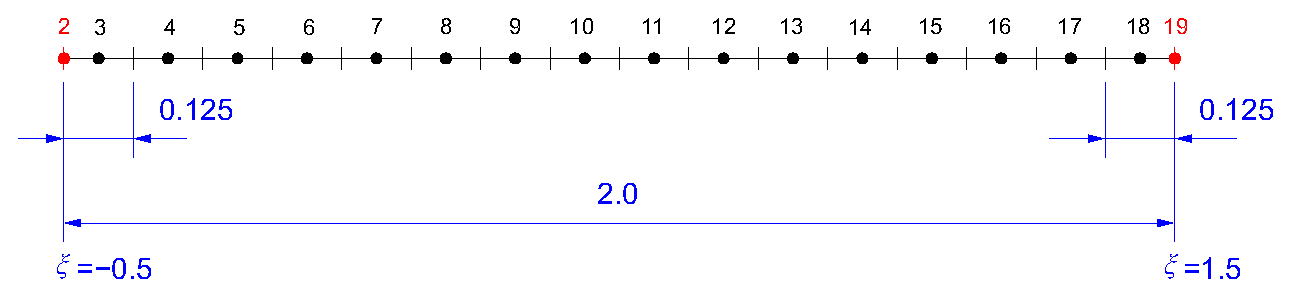
\includegraphics[scale=0.5]{Figures/05-01-grid.eps}}
  \end{picture}
  \caption{Uniform one-dimensional grid: 
                         $\bullet$ domain cells,
                         $+$       domain nodes,
                         \textcolor{red}{$\bullet$} boundary cells,
                         \textcolor{red}{$+$}       boundary nodes.
           Coordinates and dimensions are in blue.}
  \label{fig_uniform_grid}
\end{figure}

The grid created by this program is shown in Fig.~\ref{fig_uniform_grid}. 
First thing worth nothing is that there are~16 cells inside the domain (shown
by black dots and numbered from 1-16). But, in addition to cells in the
domain, {\psiboil} creates additional cells at the boundaries (red dots,
numbered 0 and 17). These {\em boundary} cells hold the values of boundary 
conditions or serve as {\em buffer} cells for parallel version. Note that,
for the case of non-periodic grid, boundary cells coincide with boundary
nodes.

If you would like to check all coordinates in the grid, un-comment line~14
and the program will write node, cell coordinates, as well as cell dimensions
on the terminal.
For a qualitative visual observation, un-comment line~15. The program will 
create an {\tt eps} figure in file {\tt grid.eps}. Both of these functions
({\tt print()} and {\tt plot(char * name)}) are used quite seldomly. Grid is
usually checked later in a post-processing package, after the {\tt Domain}
has been generated.

\subsection{Periodic grid}
\label{sub_sec_periodic}

If you want to create a periodic, line~12 from the above program should be 
changed to ({\tt 05-02-main.cpp}):
%
{\small \begin{verbatim}
     11   /* periodic grid */
     12   Grid1D grid( Range<real>(-0.25*L, 0.75*L), N, Periodic::yes());
\end{verbatim}}
%
This program, when compiled and ran, creates the grid shown in 
Fig.~\ref{fig_periodic_grid}. Dimensions of the domain cells are the same
as in previous example, but boundary cells do {\em not} coincide any
longer with boundary nodes. Boundary cell~0 is now a copy of domain
cell~16, shifted by $L$ in negative $\xi$ direction, while cell~17 is
a copy of cell~1, shifted by $L$ in positive $\xi$ direction. 

%-----------------%
%                 %
%  Periodic Grid  %
%                 %
%-----------------%
\begin{figure}[ht]
  \centering
  \setlength{\unitlength}{1mm}
  \begin{picture}(110,25)(0,0)
    \thickbox{110}{25}
    \put( 1,0){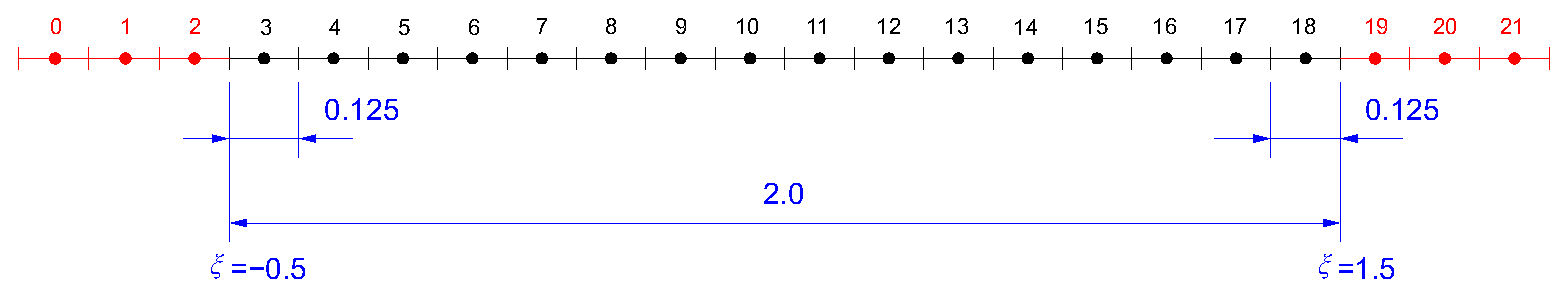
\includegraphics[scale=0.5]{Figures/05-02-grid.eps}}
  \end{picture}
  \caption{Periodic grid: $\bullet$ domain cells,
                          $+$       domain nodes,
                          \textcolor{red}{$\bullet$} boundary cells,
                          \textcolor{red}{$+$}       boundary nodes.
           Coordinates and dimensions are in blue.}
  \label{fig_periodic_grid}
\end{figure}

No matter if the grid is periodic or not, {\psiboil} adds additional cells
on the boundaries. The number of cells passed by the user, however, is 
equal to the number of {\em computational} cells. 

\subsection{Stretched grid}
\label{sub_sec_stretched}

The grids created in Sec\.~\ref{sub_sec_uniform} and~\ref{sub_sec_periodic}
were both uniform. Many problems require grid to be stretched towards
the regions where important phenomena is occurring at smaller scales to
resolve it more accurately. To create such {\em stretched} grids we need
to pass the desired cell dimension at the beginning and the end of the grid
to {\tt Grid1D}'s constructor. It is illustrated by the following program 
({\tt 05-03-main.cpp}):
%
{\small \begin{verbatim}
      1 #include "Include/psi-boil.h"
      2
      3 const real L  = 2.0;
      4 const real D1 = 0.002;
      5 const real D2 = 0.04;
      6 const int  N  = 32;
      7
      8 /****************************************************************************/
      9 main(int argc, char * argv[]) {
     10
     11   boil::timer.start();
     12
     13   /* stretched grid */
     14   Grid1D grid( Range<real>(-0.25*L, 0.75*L),
     15                Range<real>(D1, D2),
     16                N,
     17                Periodic::no());
     18
     19   grid.print();
     20
     21   boil::timer.stop();
     22   boil::timer.report();
     23 }
\end{verbatim}}
%
Stretched grid is created by calling {\tt Grid1D} constructor in lines~14--17. 
Four parameters are passed to this constructor and they represent:
%
\begin{itemize}
  \item {\tt Range<real>(-0.25*L, 0.75*L)} - start and end $\xi$ coordinate of the grid,
  \item {\tt Range<real>(D1, D2)}          - start and end cell size of the grid,
  \item {\tt N}                            - number of grid cells ({\em not} nodes),
  \item {\tt Periodic::no()}               - indicator that the grid is non-periodic.
\end{itemize}
%
First, third and fourth parameter are the same as before, while second
parameter passes the desired start and end cell size. Grid created by
the program~({\tt 05-03-main.cpp}) is illustrated in Fig.~\ref{fig_stretched_grid}. 
As you can see, the grid is stretched towards both walls, with stretching
being stronger towards the beginning of the domain.

%------------------%
%                  %
%  Stretched Grid  %
%                  %
%------------------%
\begin{figure}[ht]
  \centering
  \setlength{\unitlength}{1mm}
  \begin{picture}(110,25)(0,0)
    \thickbox{110}{25}
    \put( 1,0){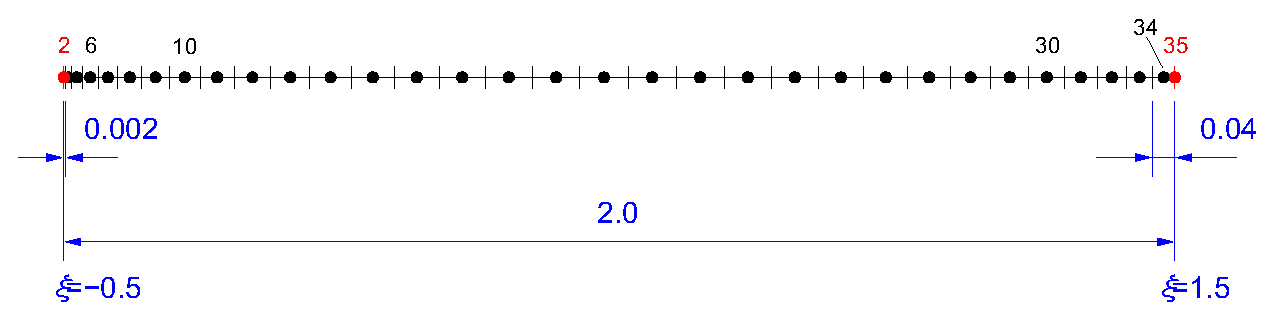
\includegraphics[scale=0.5]{Figures/05-03-grid.eps}}
  \end{picture}
  \caption{Stretched grid: $\bullet$ domain cells,
                           $+$       domain nodes,
                           \textcolor{red}{$\bullet$} boundary cells,
                           \textcolor{red}{$+$}       boundary nodes.
           Coordinates and dimensions are in blue.}
  \label{fig_stretched_grid}
\end{figure}


  \section{Ravioli classes}
\label{sec_ravioli}

Small objects, such as that of {\tt Range} type, are in {\psiboil} referred to 
as {\em ravioli} objects. They are very small and have limited functionality 
(small number of member functions), but primarily serve for improved code readability, 
safer argument passing and to reduce chances for making coding errors. 

Take class {\tt Periodic}, for example. If it was not defined, one would have
to send some other data types, such as integers, for example. Then, an
integer would be sent to {\tt Grid1D}'s constructor, having value 0 if non-periodic,
and 1 if periodic. Or, maybe, -1 if periodic and 0 if non-periodic. Such
parameters are difficult to understand, and would always have to read 
{\tt Grid1D}'s documentation to recall which number means what (Did we agree
0 was periodic, or non-periodic?). Furthermore, type checking is not ensured
with some simple types, integers and Boolean in particular. If one sends
Boolean variable as a parameter where integer should have been sent, compiler
would not notice it, resulting in hard-to-find bugs. With ravioli parameter,
compiler recognizes, during compilation time, any inconsistencies in parameter
types.  

Most frequently used ravioli classes are all declared in 
directory:~{\tt PSI-Boil/Src/Ravioli}. Those used only inside one other 
class\footnote{For example: type of preconditioner is defined as a ravioli class and is
used only inside the preconditioner class. It would not make sense to place a ravioli
class with such a limited application into~{\tt PSI-Boil/Src/Ravioli} directory.}.

More details about each of the ravioli classes can be obtained either from
it's Doxygen documentation (check the directory:~{\tt PSI-Boil/Doc/Dox}), or
from it's header file. If you find the additional information insufficient,
or even missing, feel free to contact the author. The same goes for all other
classes, of course.

%---------------------------------------------------------------------nutshell-%
\vspace*{5mm} \fbox{ \begin{minipage}[c] {0.97\textwidth} %-----------nutshell-%
    {\sf Sections \ref{sec_one-dimensional} and \ref{sec_ravioli} 
         in a nutshell} \\  %-----------------------------------------nutshell-%
    
      - {\psiboil} supports three-dimensional Cartesian grids, represent with 
      class {\tt Domain}. \\

      - {\tt Domain} is built from three one-dimensional grids 
      ({\tt Grid1D}), defining resolution in $x$, $y$ and $z$ directions. \\

      - To create a 1D grid, use the constructor: 
      \begin{itemize}
        \item {\tt Grid1D(Range<real>(xi\_s, xi\_e), N, Periodic);} 
      \end{itemize}
      for uniform grids, or: 
      \begin{itemize}
        \item {\tt Grid1D(Range<real>(xi\_s, xi\_e), Range<real>(D\_s, D\_e), N, Periodic);} 
      \end{itemize}
      for non-uniform grids. \\

      - {\psiboil} uses quite a lot of small objects, called ravioli, for
      improved code readability, safer argument passing and reduced 
      chance of coding errors. Most of them are declared in sub-directory
      {\tt Ravioli}.
   
  \end{minipage} } %--------------------------------------------------nutshell-%
%---------------------------------------------------------------------nutshell-%

  \section{Three-dimensional domains}
\label{sec_domains}

As stated before, {\psiboil} supports three-dimensional Cartesian
computational domains, defined by objects of type {\tt Domain}. 
It uses three one-dimensional grids {\tt Grid1D} to define 
resolution in each of the coordinate direction ($x$, $y$ and $z$).

The following program ({\tt 05-04-main.cpp}) creates a cubical domain, 
having dimension $1 \times 1 \times 1$, with uniform cell distribution 
in $x$ and $y$ direction, while stretched towards both ends in $z$ 
direction: 
%
{\small \begin{verbatim}
      1 #include "Include/psi-boil.h"
      2
      3 const real L = 3.2;
      4 const real D = 0.01;
      5 const int  N = 32;
      6
      7 /****************************************************************************/
      8 main(int argc, char * argv[]) {
      9
     10   boil::timer.start();
     11
     12   /* uniform grid */
     13   Grid1D g_uni( Range<real>(-0.5*L, 0.5*L), N, Periodic::no() );
     14
     15   /* stretched grid */
     16   Grid1D g_str( Range<real>(0,L), Range<real>(D,D), N*2, Periodic::no());
     17
     18   /* create domain */
     19   Domain dom(g_uni, g_uni, g_str);
     20
     21   /* plot the domain */
     22   boil::plot = new PlotTEC();
     23   boil::plot->plot(dom, "dom");
     24
     25   boil::timer.stop();
     26   boil::timer.report();
     27 }
\end{verbatim}}
%
Line~13 creates {\tt g\_uni}, a uniform grid with~32 cells, ranging 
from~$\xi=-1.6$ to $\xi=1.6$. Line~16 creates {\tt g\_str}, a grid ranging from 
$\xi=0$ to $\xi=3.2$ which is stretched towards both ends. Note that the size of
cells next to the boundaries of {\tt g\_str} is~$\Delta \xi = 0.01$. 

Command which creates the computational domain is in line~19. This line creates
an object of type~{\tt Domain}, called~{\tt dom}. It's constructor accepts three
arguments: grid in $x$, $y$ and $z$ direction. In this particular case, we use
grid~{\tt g\_uni} for distribution in $x$ and $y$, and grid~{\tt g\_str} to
define distribution in~$z$ direction.

Domain is plotted in lines~21--23. Plotting is performed with the global {\psiboil}
object~{\tt boil::plot}. This global object can be created in two ways, depending
on the format of output files you would like to create. If you would like to plot
your grids (and later results) in Tecplot\footnote{Tecplot is a registered trademark
of Tecplot Inc.\ ({\tt www.tecplot.com})} format,create the {\tt boil::plot} as 
in line~22.

The Tecplot format file, which is output from PSI-Boil, can be opened by the 
visualization software e.g. Tecplot, Paraview\footnote{\ {\tt www.paraview.org}} 
and VisIt\footnote{\ {\tt visit-dav.github.io/visit-website/}}. 
The details of post-process will be provided in Section ~\ref{chap_post_process}.


When running the program~{\tt 05-04-main.cpp}, you will get the following output:
%
{\small \begin{verbatim}
Domain level 4 created !
Domain level 3 created !
Domain level 2 created !
Domain level 1 created !
# Plotting: dom_p000.dat
+==========================================
| Total execution time: 0.18 [s]
+------------------------------------------
| Time spent in plotting: 0.18 [s]    (100%)
| Time spent elsewhere: 0 [s]    (0%)
+------------------------------------------
\end{verbatim}}
%
The output informs you that it has created four grid levels in addition to the
one specified by the user. The level specified by the user is always level~0,
while the coarser levels have larger numbers. Thus, for this particular case,
level~0 will have resolution of:~$32 \times 32 \times 64$, 
level~1: $16 \times 16 \times 32$, level~2: $8 \times 8 \times 16$, 
level~3: $4 \times 4 \times 8$ and, finally, level~4 will have the coarsest 
resolution of only $4 \times 4 \times 4$ cells. 

The grid on the finest level (level~0) is plotted from line~23, using the global
object~{\tt boil::plot} and its member function {\tt boil::plot->plot()}. As the
arguments, you send the {\tt Domain} to be plotted (in this case it is {\tt dom})
and the name you want to associate with it ({\tt "dom"}). The plotting function
({\tt boil::plot->plot()}) names the output file as: {\tt dom\_p000.dat}, where
{\tt \_p000} is processor number and {\tt .dat} is extension recognized by
Tecplot. The grid on the finest level, visualized by Tecplot is shown in 
Fig.~\ref{fig_domain_l0}. 

%----------%
%          %
%  Domain  %
%          %
%----------%
\begin{figure}[ht]
  \centering
  \setlength{\unitlength}{1mm}
  \begin{picture}(80,65)(0,0)
    \thickbox{80}{65}
    \put(0,0){\includegraphics[scale=0.33]{Figures/05-04-domain-l0.eps}}
  \end{picture}
  \caption{Stretched computational domain.}
  \label{fig_domain_l0}
\end{figure}

Note that program reports on the time spent in plotting functions with:
%
{\small \begin{verbatim}
| Time spent in plotting: 0.18 [s]    (100%)
\end{verbatim}}
%
That is because all the plotting functions are embedded in {\em local} 
timing routines, such as the ones introduced in the section~\ref{sec_local}.

You have to stretch the grid towards the walls very often, but sometimes
you might also want to stretch in the interior - particuluarly if there
are obstacles (or inner walls) inside. A way to achieve such a stretching
is to combine two stretched grids together. The way to do it is demostrated
below. The lines of the {\tt 05-04-main.cpp} code are replaced with the 
following (to get the program {\tt 05-05-main.cpp}):
%
{\small \begin{verbatim}
     15   /* stretched grid */
     16   Grid1D g_str( Range<real>(0,0.5*L), Range<real>(D,D), N, Periodic::no());
     17
     18   Grid1D g_str_2(g_str, g_str, Periodic::no());
     19
     20   /* create domain */
     21   Domain dom(g_uni, g_uni, g_str_2);
\end{verbatim}}
%
{\tt Grid1D g\_str} is still created in line~16, but this time is half
as short and it has half as many cells as in the previous case. Next,
additional grid is created in line~18, where two {\tt g\_str}'s are
added one after another. The {\tt Grid1D} constructor in line~18 
takes two {\tt Grid1D}'s as parameters, leaves the absolute coordinates
of the first intact, but disregards the absolute coordinates of the second.
It shifts and attaches the grid sent as second parameter to the grid sent
as first parameter\footnote{If it was not shifting the second, they
would collapse into one grid for this case.}. 
Finally, {\tt Domain dom} is created in line~21 using the new,
double-stretched grid to set the resolution in~$z$ direction, and
is plotted in~Fig.~\ref{fig_domain_double_stretched}. 

%
%----------------------------%
%                            %
%  Domain - duble stretched  %
%                            %
%----------------------------%
\begin{figure}[ht]
  \centering
  \setlength{\unitlength}{1mm}
  \begin{picture}(80,65)(0,0)
    \thickbox{80}{65}
    \put(0,0){\includegraphics[scale=0.33]{Figures/05-04-double-stretch.eps}}
  \end{picture}
  \caption{Double-stretched computational domain.}
  \label{fig_domain_double_stretched}
\end{figure}

% remove? \subsection{Implicit plotting}
% remove? 
% remove? In the program example {\tt 05-04-main.cpp} you have explicitly 
% remove? plotted the computational domain from lines~21--23. This plotted only
% remove? the finest grid level. There is a way to plot coarser grid levels as
% remove? well. To achieve that, remove lines 21 and 22 from~{\tt 05-04-main.cpp}
% remove? and move the line~23 above the definition of the {\tt Domain dom}.
% remove? You might even place it just after starting the timer (line~10), to 
% remove? get the listing ({\tt 05-05-main.cpp}):
% remove? %
% remove? {\small \begin{verbatim}
% remove?       1 #include "Include/psi-boil.h"
% remove?       2
% remove?       3 const real L = 3.2;
% remove?       4 const real D = 0.01;
% remove?       5 const int  N = 32;
% remove?       6
% remove?       7 /****************************************************************************/
% remove?       8 main(int argc, char * argv[]) {
% remove?       9
% remove?      10   boil::timer.start();
% remove?      11
% remove?      12   /* plot in Tecplot format */
% remove?      13   boil::plot = new PlotTEC();
% remove?      14
% remove?      15   /* uniform grid */
% remove?      16   Grid1D g_uni( Range<real>(-0.5*L, 0.5*L), N, Periodic::no() );
% remove?      17
% remove?      18   /* stretched grid */
% remove?      19   Grid1D g_str( Range<real>(0,L), Range<real>(D,D), N*2, Periodic::no());
% remove?      20
% remove?      21   /* create domain */
% remove?      22   Domain dom(g_uni, g_uni, g_str);
% remove?      23
% remove?      24   boil::timer.stop();
% remove?      25   boil::timer.report();
% remove?      26 }
% remove? \end{verbatim}}
% remove? %
% remove? When compiled and ran, this program creates the output:
% remove? %
% remove? {\small \begin{verbatim}
% remove? Domain level 4 created !
% remove? # Plotting: domain_p000_0004.dat
% remove? Domain level 3 created !
% remove? # Plotting: domain_p000_0003.dat
% remove? Domain level 2 created !
% remove? # Plotting: domain_p000_0002.dat
% remove? Domain level 1 created !
% remove? # Plotting: domain_p000_0001.dat
% remove? # Plotting: domain_p000_0000.dat
% remove? +==========================================
% remove? | Total execution time: 0.22 [s]
% remove? +------------------------------------------
% remove? | Time spent in plotting: 0.22 [s]    (100%)
% remove? | Time spent elsewhere: 0 [s]    (0%)
% remove? +------------------------------------------
% remove? \end{verbatim}}
% remove? %
% remove? This time it plotted each domain level it created, from finest level, stored
% remove? in file {\tt domain\_p000\_0000.dat}, to the coarsest one stored in
% remove? {\tt domain\_p000\_0004.dat}. The four-digit number before the file extension
% remove? denotes the grid level. 
% remove? For example, level~2 is shown in Fig.~\ref{fig_domain_l2}.
% remove? 
% remove? %----------%
% remove? %          %
% remove? %  Domain  %
% remove? %          %
% remove? %----------%
% remove? \begin{figure}[ht]
% remove?   \centering
% remove?   \setlength{\unitlength}{1mm}
% remove?   \begin{picture}(80,65)(0,0)
% remove?     \thickbox{80}{65}
% remove?     \put(0,0){\includegraphics[scale=0.33]{Figures/05-05-domain-l2.eps}}
% remove?   \end{picture}
% remove?   \caption{Computational domain at level 2, visualized with Tecplot.}
% remove?   \label{fig_domain_l2}
% remove? \end{figure}
% remove? 
% remove? This {\em implicit} plotting was introduced in early stages of {\psiboil} 
% remove? development, when the main concern was the multigrid solver. If it annoys you,
% remove? simply define {\tt boil::plot} after the definition of a {\tt Domain} and
% remove? {\psiboil} will not do it. 

%---------------------------------------------------------------------nutshell-%
\vspace*{5mm} \fbox{ \begin{minipage}[c] {0.97\textwidth} %-----------nutshell-%
    {\sf Section \ref{sec_domains} in a nutshell} \\  %---------------nutshell-%
   
      - Three-dimensional Cartesian grids, represent with class {\tt Domain}, 
      are created from three one-dimensional grids ({\tt Grid1D}), with 
      the constructor:
      \begin{itemize}
        \item {\tt Domain(Grid1D \& gx, Grid1D \& gy, Grid1D \& gz);}
      \end{itemize}
      where {\tt gx}, {\tt gy} and {\tt gz} represent grid resolutions
      in $x$, $y$ and $z$ coordinate directions. \\
  
      - In order to plot domains, global object {\tt boil::plot} must be 
      defined before it is used. \\
 
      - {\tt boil::plot} can be defined as:
      \begin{itemize}
        \item {\tt boil::plot = new PlotTEC();} for plotting with Tecplot.
      \end{itemize}

      - Grids ({\tt Grid1D}) can also be constructed by appending one
      after another, using the constructor: 
      {\tt Grid1D(Grid1D \&, Grid1D \&, Periodic)}. \\

      - {\tt Domain}s can be plotted explicitly, using the command:
      \begin{itemize}
        \item {\tt boil::plot->plot(Domain \& dom, "file\_name");}
      \end{itemize}
% remove?       or implicitly, just by defining {\tt boil::plot} before the
% remove?       {\tt Domain}.
    
  \end{minipage} } %--------------------------------------------------nutshell-%
%---------------------------------------------------------------------nutshell-%

  \section{Immersed Bodies}
\label{sec_boddies}

One of the distinct features of {\psiboil} is it's ability to solve problems in
complex computational domains using an immersed boundary method~(IBM). For such cases, 
computational domain is divided into a {\em fluid} part, where all governing 
equations for heat transfer and fluid flow are solved, and the {\em solid} part, 
where no momentum equations are solved. However, in case of conjugate heat transfer
problems, heat transfer equations is solved in the solid part as well. 

In {\psiboil} solid parts of the computational domain are defined as
{\em immersed boundaries}, represented by the class {\tt Body}. These immersed
bodies (IB's) are defined by a computer aided design~(CAD) files in 
ASCII stereolitography~(STL) format. The creation of CAD files is performed by
a third party program. At PSI we use AC3D\footnote{\tt http://www.inivis.com/}, 
but any other CAD software package able to export ASCII STL file format could be used. 
This tutorial does not cover the usage of AC3D, nor any other CAD packages. It is
important, however, to mention the convention adopted in {\psiboil} concerning
IB's: {\em normals on the body surface point to the fluid part
of the domain}.

The usage of IB is illustrated in the following example. Consider a case of a domain
with dimensions: $4 \times 1 \times 1$ in $x$, $y$ and $z$ direction
respectively, with a step-like obstacle with dimension 
$0.5 \times 1.0 \times 0.5$ placed at the bottom wall (minimum $z$) 
of the domain. Immersed body is created in AC3D and stored in the file named {\tt step.stl}.
The dimensions of the IB are set to be slightly larger in CAD program
to avoid ambiguity when cutting cells. In effect, the actual dimensions of the IB are
$0.501 \times 1.001 \times 0.501$.
This file should be stored in the running directory. The program which uses the~STL
file to create a mesh for a domain with a step-like obstacle is ({\tt 05-06-main.cpp}): 
%
{\small \begin{verbatim}
      1 #include "Include/psi-boil.h"
      2
      3 const real LX = 4.0;
      4 const real LY = 1.0;
      5 const int  NX =  64;
      6 const int  NY =  16;
      7
      8 /******************************************************************************/
      9 main(int argc, char * argv[]) {
     10
     11   boil::timer.start();
     12
     13   /* plot in Tecplot format */
     14   boil::plot = new PlotTEC();
     15
     16   /* grids */
     17   Grid1D g_x( Range<real>(0,LX), NX, Periodic::no() );
     18   Grid1D g_y( Range<real>(0,LY), NY, Periodic::no() );
     19
     20   /* create immersed body */
     21   Body step("05-06-step.stl");
     22
     23   /* plot step before immersion */
     24   boil::plot->plot(step, "step-before");
     25
     26   /* create domain */
     27   Domain dom(g_x, g_y, g_y, &step);
     28
     29   /* plot step after immersion */
     30   boil::plot->plot(step, "step-after");
     31
     32   /* plot domain after immersion */
     33   boil::plot->plot(dom, "dom-after");
     34
     35   boil::timer.stop();
     36   boil::timer.report();
     37 }
\end{verbatim}}
%
Program lines from~1--18 should be clear at this point. {\tt Body} is created
in line 21. It is defined with the STL file name containing IB definition. As soon
as the {\tt Body} is created, it is plotted from line~24. This plotting is not
necessary, of course, but can be useful for checking. 

Problem domain is defined in line~27. The novelty in this constructor is the 
final argument, a reference to {\tt Body} (an IB). {\tt Domain}'s constructor will cut 
the computational cells with IB, but also change the IB itself. 
Line~30 plots the IB after cutting and line~33 the final computational domain.
If you compile and run this program, it will create the following output:
%
{\small \begin{verbatim}
# Plotting: step-before_p000.dat
Domain level 4 created !
Domain level 3 created !
Domain level 2 created !
Domain level 1 created !
# Plotting: sca_p000.dat
# Plotting: vec_p000.dat
# Plotting: step-after_p000.dat
# Plotting: dom-after_p000.dat
+==========================================
| Total execution time: 0.29 [s]
+------------------------------------------
| Time spent in plotting    : 0.24 [s]    (82.7586%)
| Time spent in bounding box: 0 [s]    (0%)
| Time spent in cell cutting: 0.02 [s]    (6.89655%)
| Time spent in flood fill  : 0.01 [s]    (3.44828%)
| Time spent elsewhere      : 0.02 [s]    (6.89655%)
+------------------------------------------
\end{verbatim}}
%
File containing IB before immersing (cutting) is called {\tt step-before\_p000.dat},
while the IB after immersing is stored in file {\tt step-after\_p000.dat}. They are
plotted in Figs.~\ref{fig_body_before} and~\ref{fig_body_after}, respectively. 

%--------%
%        %
%  Body  %
%        %
%--------%
\begin{figure}[ht!]
  \centering
  \setlength{\unitlength}{1mm}
  \begin{picture}(103,53)(0,0)
    \thickbox{103}{53}
    \put(0,-20){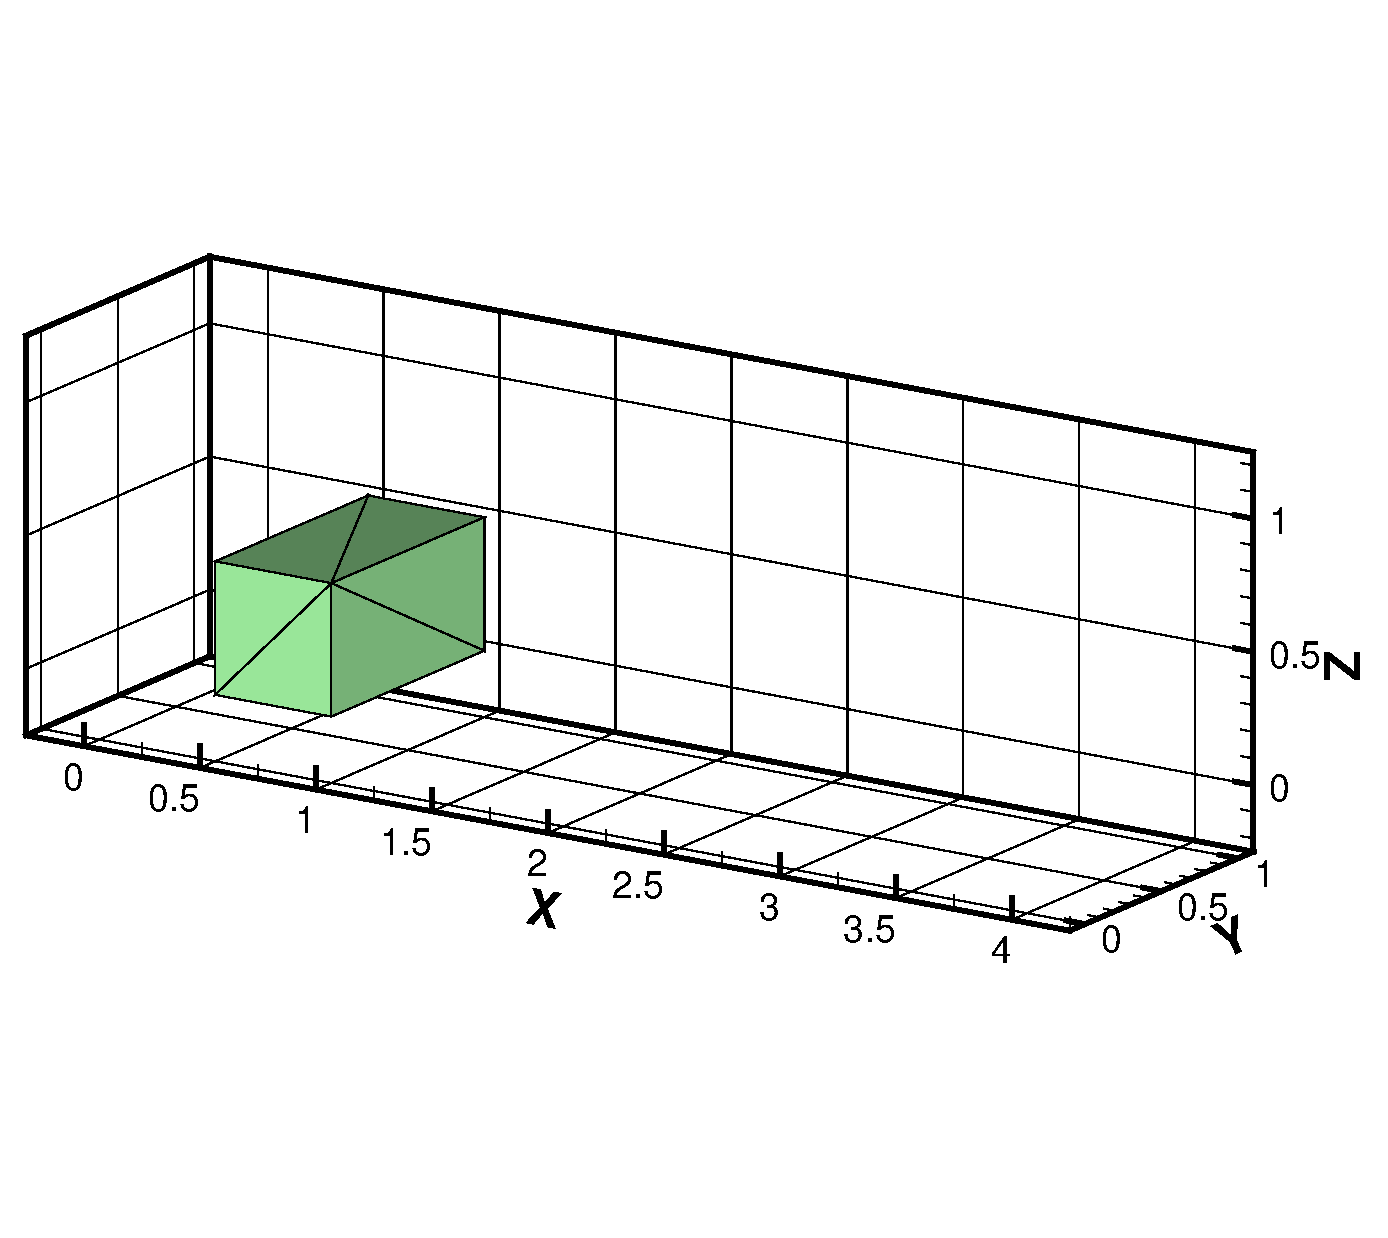
\includegraphics[scale=0.45]{Figures/05-06-body-before.eps}}
  \end{picture}
  \caption{IB plotted from line~24, {\em i.e.} before immersing it into
           computational domain. At this point it is the same as it was 
           defined in a CAD program.}
  \label{fig_body_before}
\end{figure}

In addition to the IB and domain files described above, {\psiboil} creates two
additional files: {\tt sca\_p000.dat} and {\tt vec\_p000.dat}. These files hold
scalar and vector respectively, representing ratio of the computational cell 
volume immersed in fluid. So, for cells inside the fluid part of the domain, 
it's value is~$1$, in the solid part it is~$0$, and for cells which are cut by 
immersed body, it's value is between~$0$ and~$1$. {\tt sca\_p000.dat} holds these 
values for scalar variables, while {\tt vec\_p000.dat} holds vector values. It is
a good practice to visualize these fields, just to visually check if IB is 
properly handled by {\psiboil}. Visualization of~{\tt sca\_p000.dat} is given
in Fig.~\ref{fig_scalar_obst_1}.

%--------%
%        %
%  Body  %
%        %
%--------%
\begin{figure}
  \centering
  \setlength{\unitlength}{1mm}
  \begin{picture}(103,53)(0,0)
    \thickbox{103}{53}
    \put(0,-20){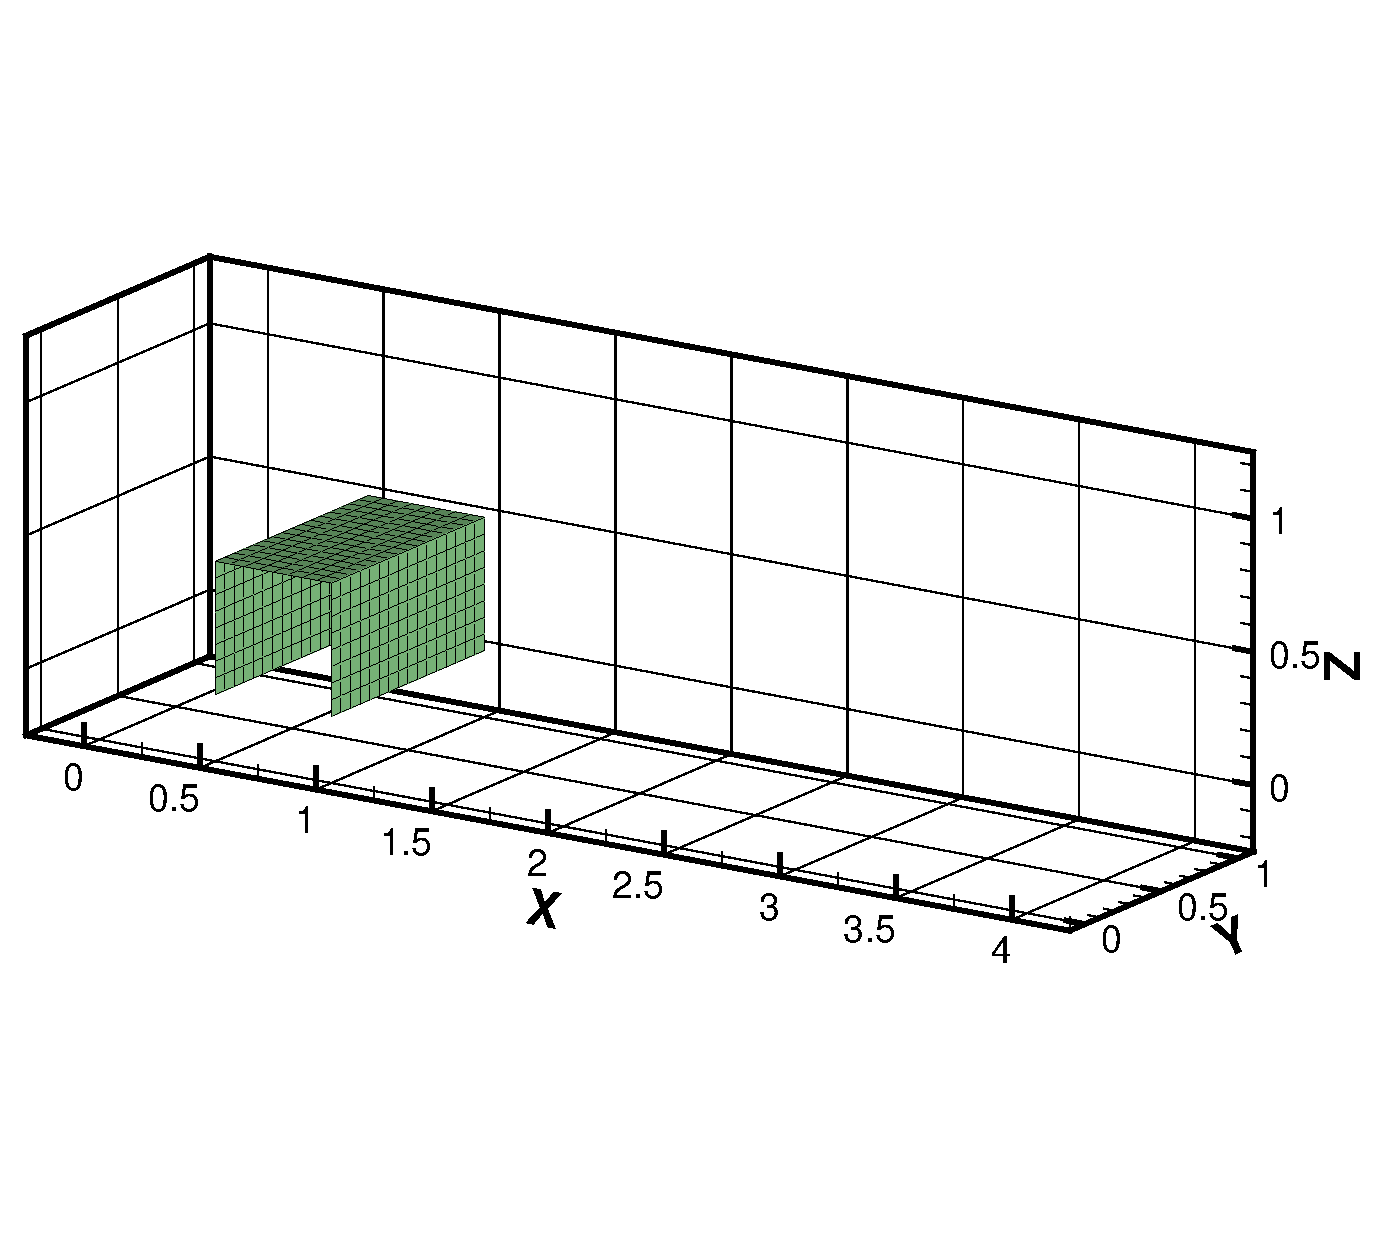
\includegraphics[scale=0.45]{Figures/05-07-body-after.eps}}
  \end{picture}
  \caption{IB plotted from line~30, {\em i.e.} after immersing it into
           computational domain. At this point, the topology of the IB  
           has changed; the original triangles are replaced by cell cuts.}
  \label{fig_body_after}
\end{figure}

%----------%
%          %
%  Domain  %
%          %
%----------%
\begin{figure}
  \centering
  \setlength{\unitlength}{1mm}
  \begin{picture}(103,53)(0,0)
    \thickbox{103}{53}
    \put(0,-20){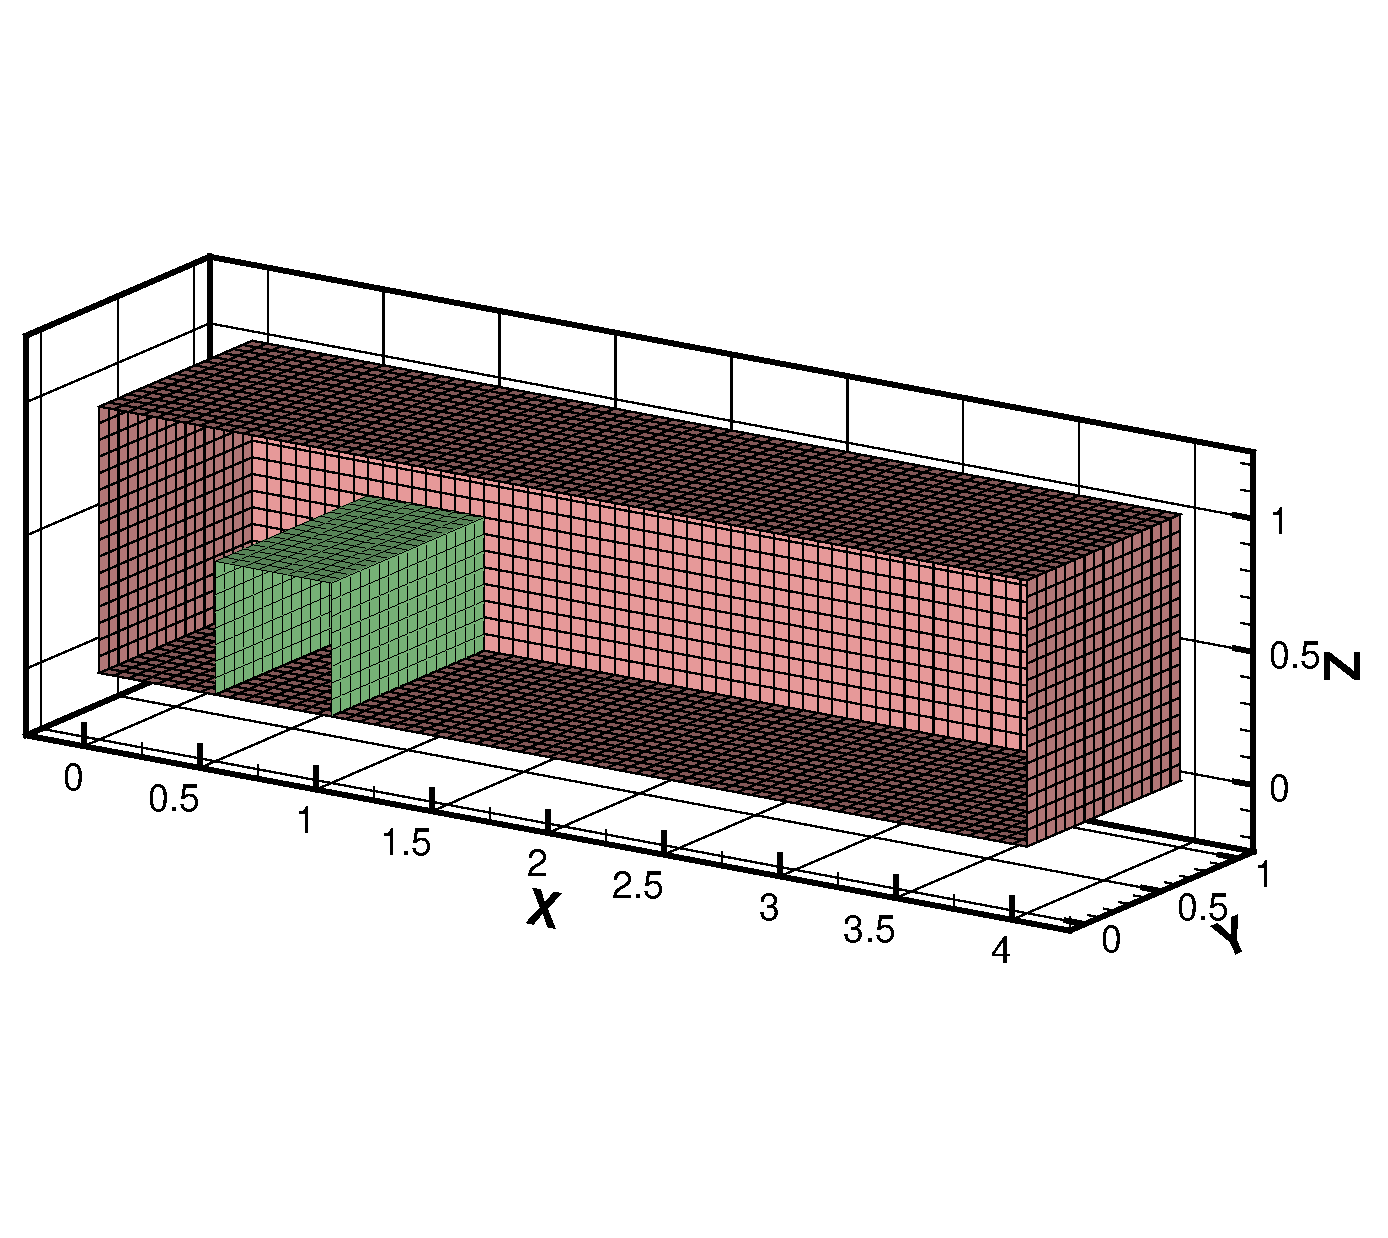
\includegraphics[scale=0.45]{Figures/05-08-domain.eps}}
  \end{picture}
  \caption{Computational domain with IB. Domain is colored in pink and obstacle 
           in green. The front face is removed from the figure for the sake of clarity.}
  \label{fig_domain_obst_1}
\end{figure}

%----------%
%          %
%  Scalar  %
%          %
%----------%
\begin{figure}
  \centering
  \setlength{\unitlength}{1mm}
  \begin{picture}(103,53)(0,0)
    \thickbox{103}{53}
    \put(0,-20){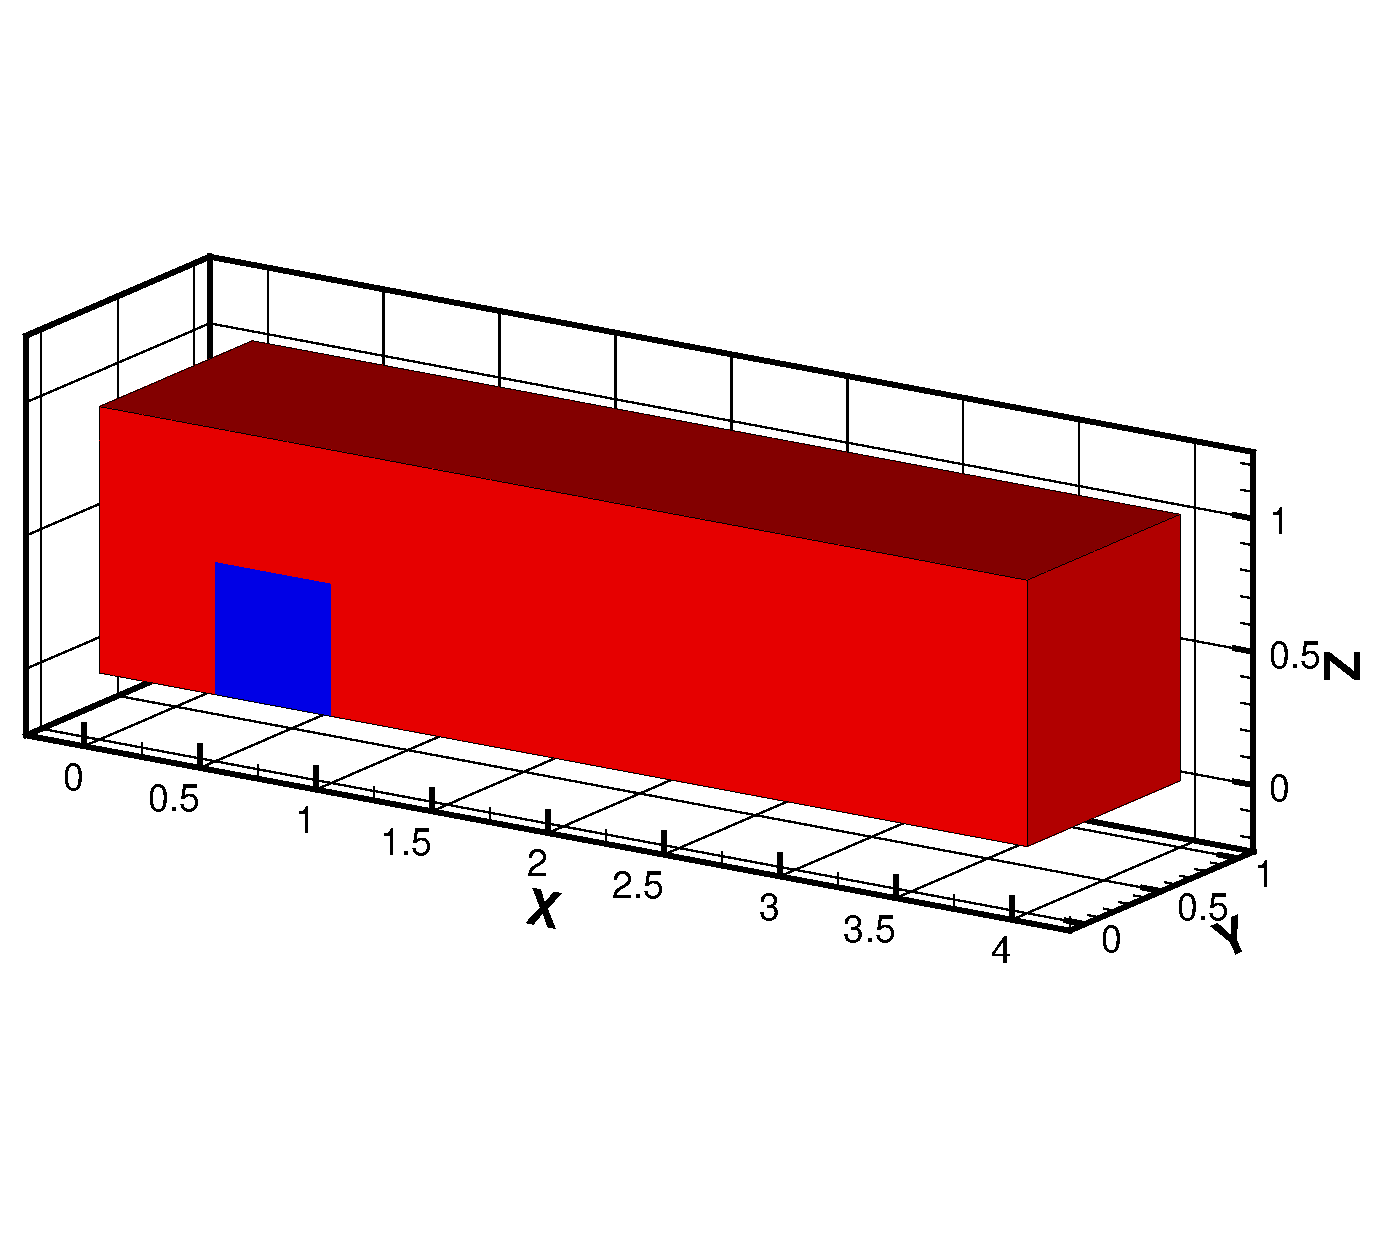
\includegraphics[scale=0.45]{Figures/05-09-sca.eps}}
  \end{picture}
  \caption{Scalar field representing volume fraction of the cell immersed in fluid.}
  \label{fig_scalar_obst_1}
\end{figure}

%---------------------------------------------------------------------nutshell-%
\vspace*{5mm} \fbox{ \begin{minipage}[c] {0.97\textwidth} %-----------nutshell-%
    {\sf Section \ref{sec_boddies} in a nutshell} \\  %-------------nutshell-%
    
      - To deal with problems in complex geometries, {\psiboil} divides computational 
      {\tt Domain} into {\em fluid} and {\em solid} part. \\

      - Solid part is represented with an object of type {\tt Body}, while fluid
      is everywhere else. \\

      - By convention, the CAD file representing the {\tt Body} has surface 
      normals oriented toward the fluid part of the computational domain. \\

      - {\tt Body} is an object created from a 3D CAD file as following:
      \begin{itemize}
        \item {\tt Body body(const std::string name);}  
      \end{itemize}
      where {\tt name} is the name of the CAD file in ASCII STL format. \\

      - {\tt Body} is inserted into a {\tt Domain}, using the constructor:
      \begin{itemize}
        \item {\tt Domain(Grid1D \&, Grid1D \&, Grid1D \&, Body *);}
      \end{itemize}
      {\tt Body} is sent as a pointer to {\tt Domain} because it changes 
      during the process of computational cell cutting.
   
  \end{minipage} } %--------------------------------------------------nutshell-%
%---------------------------------------------------------------------nutshell-%

  \section{Domain decomposition}
\label{sec_decomposition}

Run the previous program ({\tt 05-06-main.cpp}) in parallel on two processors. 
As a reminder, you do it with:
%
\begin{verbatim}
> mpirun -np 2 ./Boil
\end{verbatim}
%
The program will create the following output:
%
{\small \begin{verbatim}
# Plotting: step-before_p000.dat
# Plotting: step-before_p001.dat
Domain level 3 created !
Domain level 2 created !
Domain level 1 created !
# Plotting: sca_p000.dat
# Plotting: vec_p000.dat
# Plotting: sca_p001.dat
# Plotting: vec_p001.dat
# Plotting: step-after_p000.dat
# Plotting: dom-after_p000.dat
# Plotting: step-after_p001.dat
# Plotting: dom-after_p001.dat
+==========================================
| Total execution time: 0.175 [s]
+------------------------------------------
| Time spent in plotting    : 0.13 [s]    (74.2857%)
| Time spent in bounding box: 0 [s]    (0%)
| Time spent in cell cutting: 0.015 [s]    (8.57143%)
| Time spent in flood fill  : 0.02 [s]    (11.4286%)
| Time spent elsewhere      : 0.01 [s]    (5.71429%)
+------------------------------------------
\end{verbatim}}
%
(Remember that domains are plotted implicitly, without direct invocation).
You get two domains, one for each processor. Namely, the grids are stored
in {\tt dom-after\_p000.dat} for processor~0 and {\tt dom-after\_p001.dat}
for processor~1. These two grids are shown in Fig.~\ref{fig_domain_decomp}.

%----------%
%          %
%  Domain  %
%          %
%----------%
\begin{figure}[ht]
  \centering
  \setlength{\unitlength}{1mm}
  \begin{picture}(130,47)(0,0)
    \thickbox{130}{47}
    \put( 0,-27){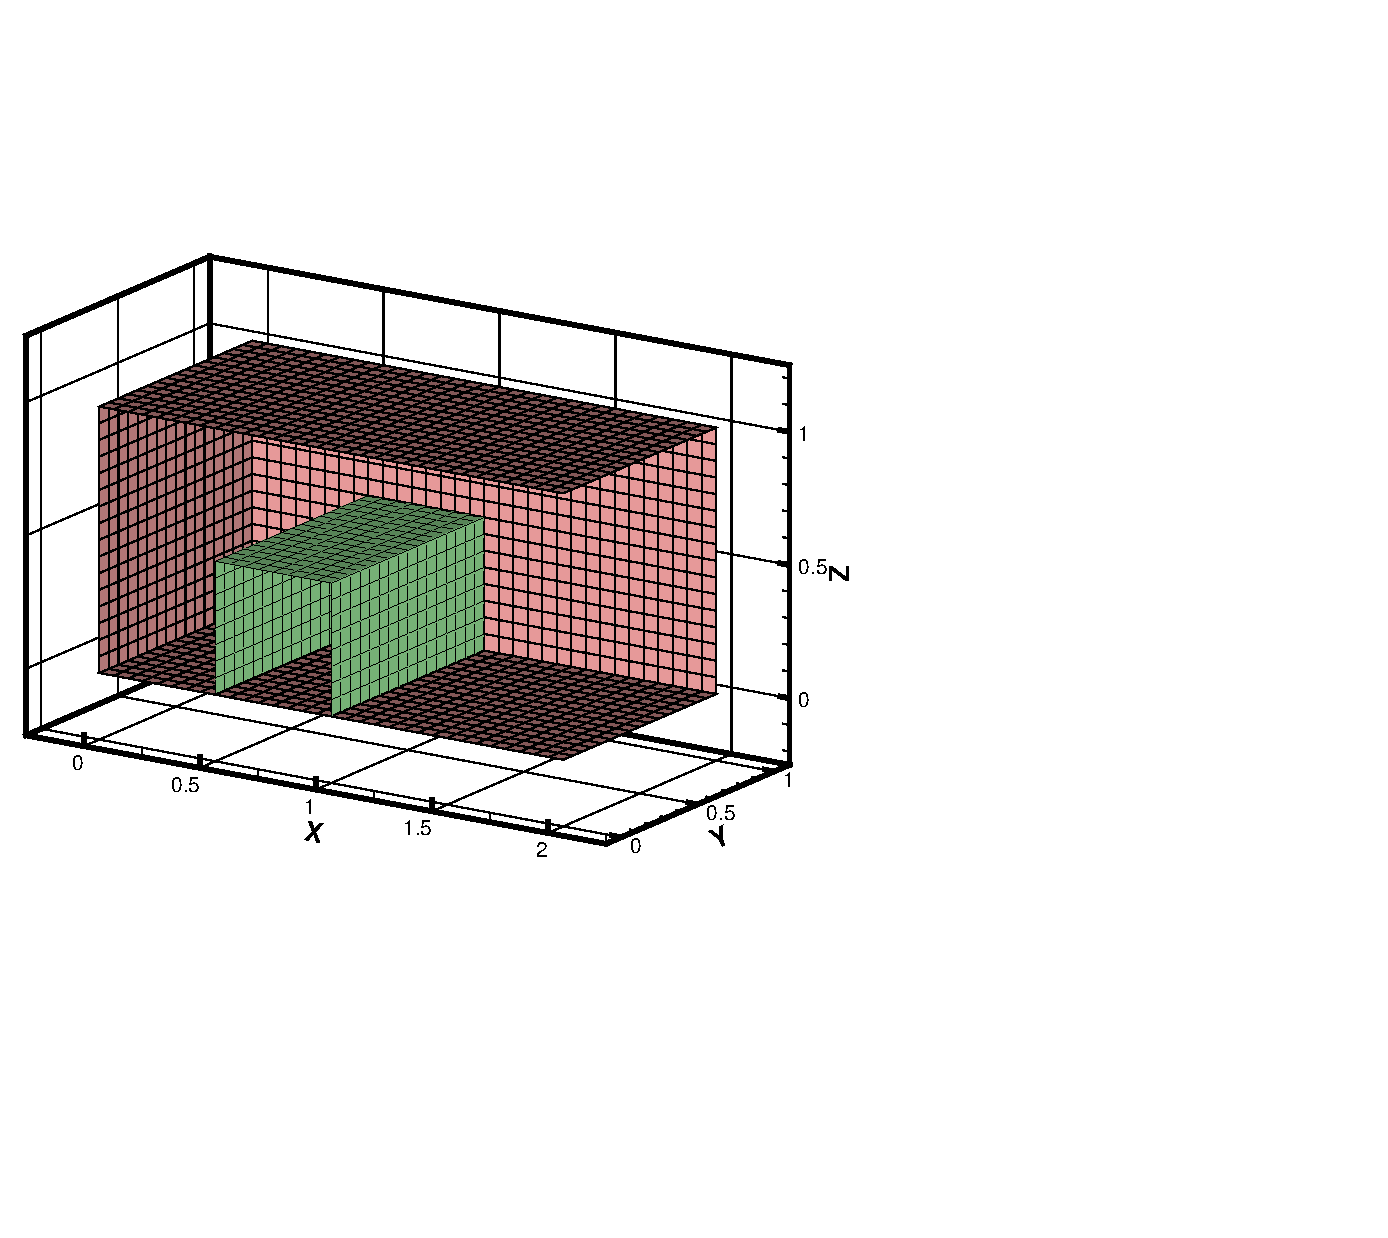
\includegraphics[scale=0.45]{Figures/05-10-par-0.eps}}
    \put(30,-21){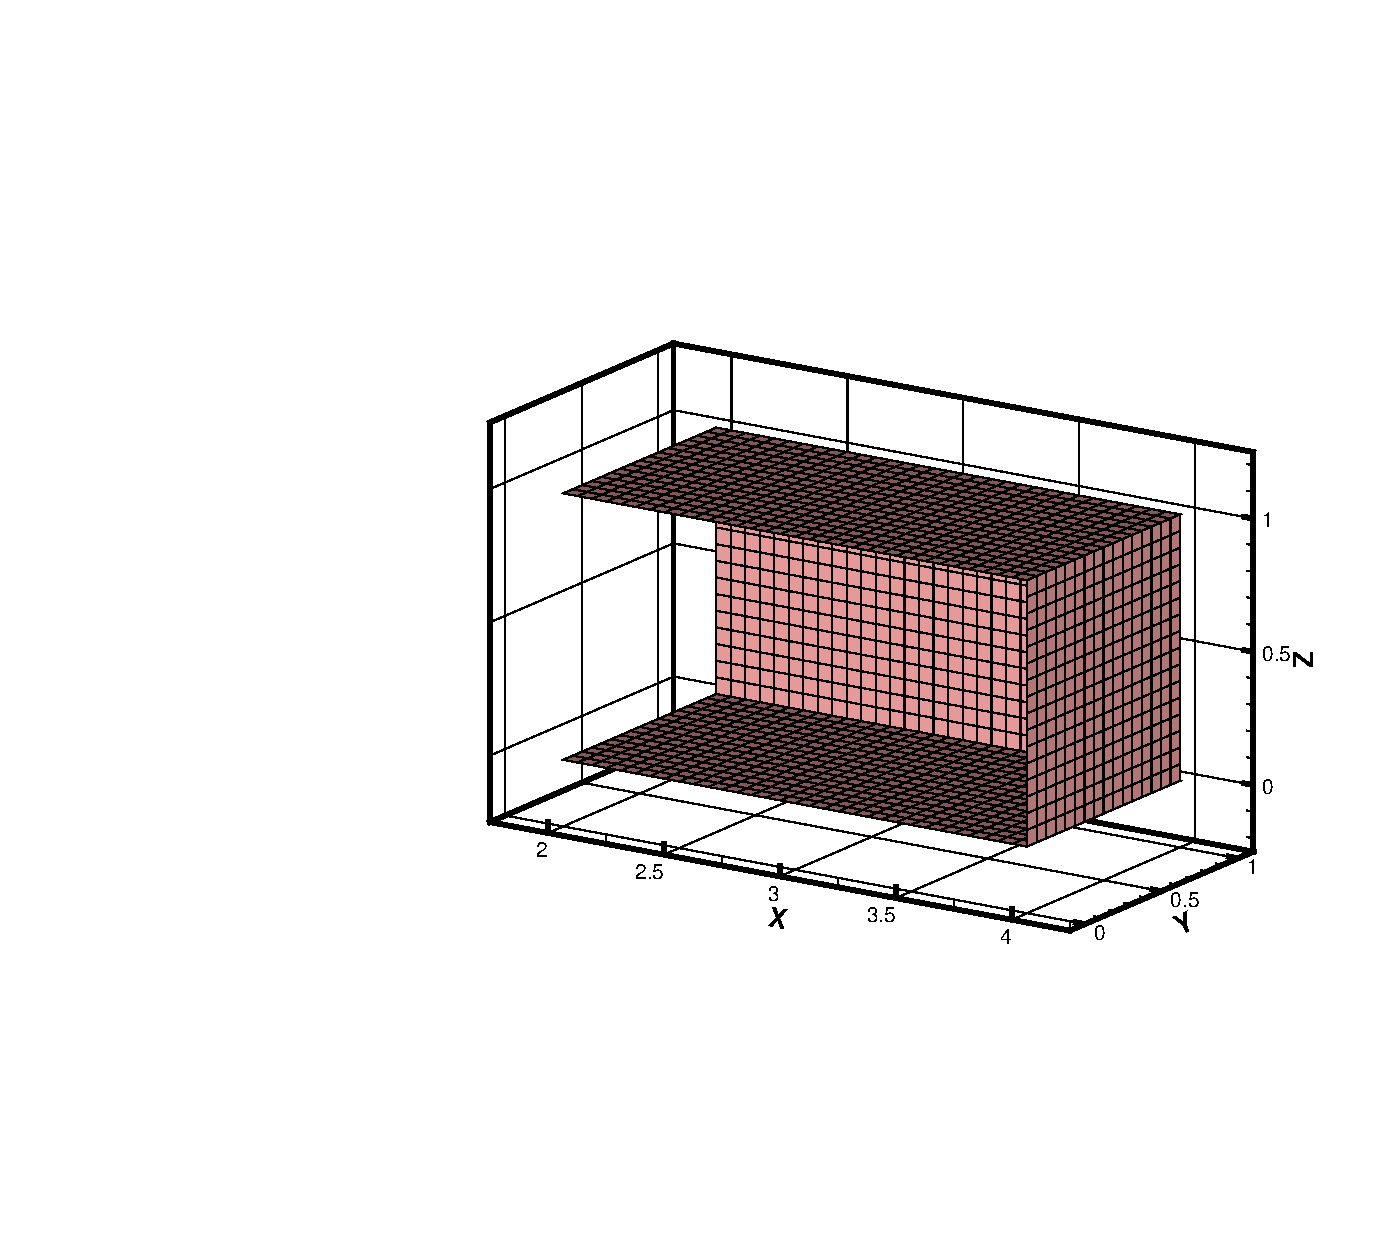
\includegraphics[scale=0.45]{Figures/05-10-par-1.eps}}
  \end{picture}
  \caption{Computational domain decomposed in two sub-domains.
           The front face, as well as the face between the sub-domains 
           are removed from the figure for the sake of clarity.}
  \label{fig_domain_decomp}
\end{figure}

While it is undoubtedly interesting to see the decomposed computational
domain, it is of little practical value. Much more often one wants to 
see the entire computational domain, together with solutions of governing
equations on it. {\psiboil}, if ran in parallel, plots as many domains
and result files as there were processors used. That is the simplest,
but also the most efficient way to parallelize file output. To connect
the files, we use an external program, called {\tt Connect}\footnote{It
was possible to create {\psiboil} in such a way that it creates a single
result file, no matter how many processors have been used. But, that would
put additional burden on parallel efficiency of {\psiboil}, only to make
post-processing more convenient for the user. It does not make sense to
sacrifice efficiency for convenience, particularly for an academic code
such as {\psiboil}, which is not meant to beat commercial CFD packages
in user-friendliness, or convenience.} 

{\tt Connect} is a part of {\psiboil} package, and resides in directory:
{\tt PSI-Boil/Src/Connect}, hereafter referred to as {\em connect}
directory. If you followed the instructions for creating
{\tt Makefile}s (Sec.~\ref{sub_sec_creating_makefiles}), there should 
already be a {\tt Makefile} in connect directory. Go there and run
{\tt make}. After a short compilation, an executable with the name 
{\tt Connect} is created. Go back to source and run:
%
\begin{verbatim}
> ./Connect/Connect
\end{verbatim}
%
It will print short message with outlining program usage, namely:
%
{\small \begin{verbatim}
Usage:
Connect/Connect <base_name> <ext> <number_of_processor> [time_step/level]
\end{verbatim}}
%
The first item being printed is the {\tt Connect} program name with full
path. It is followed by command line arguments, which are:
%
\begin{itemize}
  \item {\tt base\_name} - name assigned in call to plotting functions
        In the present case, it is {\tt domain}, implicitly defined
        by {\psiboil}.
  \item {\tt ext} - file extension, determining the file type being connected. 
        It may be either {\tt gmv} for GMV, or {\tt dat} for Tecplot. 
  \item {\tt number\_of\_processor} - clearly number of processors over which 
        the domain is distributed. For this case, it is~2. 
  \item {\tt time\_step/level} - the final argument which specifies the time 
        step, or grid level. This argument is optional, but for the present 
        case, grid level has to be specified. 
\end{itemize}
%
So, to connect the domain you got after the run on two processors, run:
%
\begin{verbatim}
> ./Connect/Connect dat dom 2 0
\end{verbatim}
%
and, after messages such as these:
%
{\small \begin{verbatim}
reading: dom-after_p000.dat
reading: dom-after_p001.dat
number of variables (excluding coordinates): 0
number of variables (excluding coordinates): 0
creating: dom-after.dat
body 0
present at 0
nodes 1664
cells 832
bodies finished
\end{verbatim}}
%
It will create the file {\tt dom-after.dat} which holds the single grid (not
distributed). 

%---------------------------------------------------------------------nutshell-%
\vspace*{5mm} \fbox{ \begin{minipage}[c] {0.97\textwidth} %-----------nutshell-%
    {\sf Section \ref{sec_decomposition} in a nutshell} \\  %---------nutshell-%
    
      - When ran in parallel, {\psiboil} automatically decomposes the
      the computational domain. \\

      - {\psiboil} performs separate plotting, i.e.\ each processors plots
      its own sub-domain. \\ 

      - Solid part is represented with {\tt Obstacle}s, while fluid
      is everywhere else. \\

      - Sub-domains are connected into a single file, using the program {\tt Connect},
      residing in directory {\tt PSI-Boil/Src/Connect}. \\

      - {\tt Connect} is not build by default. To build it, run {\tt make} in
      it's directory. 

  \end{minipage} } %--------------------------------------------------nutshell-%
%---------------------------------------------------------------------nutshell-%


  %----------------------------%
  %                            %
  %  Scalar and Vector Fields  %
  %                            %
  %----------------------------%
  \chapter{Scalar and Vector Fields}
  \label{chap_single_phase}

This chapter deals with the solution of transport equation for incompressible
fluid flow. The equation which describes this phenomenon is momentum
conservation equation, given by~\ref{eq_momentum}, repeated here for
convenience:
%
\be
         \int_V \frac{\p \rho \uvw}{\p t} dV
       + \int_S \rho \uvw \uvw \, dS
       = \int_S \mu \nabla \uvw \, dS
       - \int_V \nabla p \, dV
       + {\bf F}
       \; \; \; \;
       [N]
  \label{eq_momentum_2}
\ee
%
This form, however,
poses a problem. We have one three equations (one for each velocity 
component), but for unknowns: velocity components and pressure. 

For incompressible flow problems, pressure has always been sought through
additional constraint, mass conservation equation:
%
\be
       \int_V \frac{\p \rho}{\p t} dV 
       = 
       - \int_S \rho \uvw d{\bf S}
       \; \; \; \;
       [\frac{kg}{s}]
  \label{eq_mass}
\ee
% 
Momentum and mass conservation have been linked in various ways, providing
different algorithms for computation of incompressible flows. The most
widely used in applied CFD are SIMPLE, SIMPLEC, SIMPLER and even PISO 
({\bf references}). For highly unsteady flow, at simulation of which
{\psiboil} aims, the most efficient is the {\em fractional step method},
sometimes referred to as the {\em projection} method. It combines momentum
conservation equation~(\ref{eq_momentum}) with mass conservation
equation~(\ref{eq_mass}), at intermediate time between two simulated
time steps, to give additional equation for pressure (already introduced
as~\ref{eq_pressure}):
%
\be
         \int_S \frac{\nabla p}{\rho} \, d{\bf S} 
       = \frac{1}{\Delta t} \int_S \uvw^\s \, d{\bf S}
       \; \; \; \; 
       [ \frac{m^3}{s^2} ],
  \label{eq_pressure_2}
\ee
%
often referred to as pressure-Poisson equation.

The fractional step method, which is used by {\psiboil}, is now outlined.
The momentum conservation equation~(\ref{eq_momentum_2}) must first be discretized
in time, part by part. The most usual approach is to use Crank-Nicolson
scheme for diffusion (to avoid very low time steps needed by the forward
Euler scheme) and to use Adams-Bashforth for convection, for the sake
of simplicity. Inertial terms are discretized with backward Euler scheme.
The time-discretized momentum equation then looks like:
%
\be
        {\bf I}^\s - {\bf I}^{n-1} 
       + \frac{3}{2} {\bf C}^{n-1} - \frac{1}{2} {\bf C}^{n-2}
       = \frac{1}{2} {\bf D}^\s + \frac{1}{2} {\bf D}^{n-1}
       + {\bf F}^{n-1}
  \label{eq_semi}
\ee
%
Here, $\s$ denotes the tentative (intermediate) time step, while 
${\bf I}^\s = \frac{1}{\Delta t} \int_V  \rho \uvw^\s dV$ 
and ${\bf D}^\s = \int_S \mu \nabla \uvw^\s \, d{\bf S}$ 
denote inertial and diffusive term in the tentative time step. 
Old (known) values of velocity (at time step $n-1$) define terms:
${\bf I}^{n-1} = \frac{1}{\Delta t} \int_V  \rho \uvw^{n-1} dV$,
and ${\bf D}^{n-1} = \int_S \mu \nabla \uvw^{n-1} \, d{\bf S}$, as well
as convective term at old time step: 
${\bf C}^{n-1} = \int_S \rho \uvw^{n-1}\uvw^{n-1} \, d{\bf S}$. Clearly,
${\bf C}^{n-2} = \int_S \rho \uvw^{n-2}\uvw^{n-2} \, d{\bf S}$.

Equation~\ref{eq_semi} is discretized in space giving a linear system
of equations for intermediate velocity~($\uvw^\s$). Once this
system is solved gives velocity field which does not, generally, 
satisfies mass conservation equation. It is used to compute pressure 
from~\ref{eq_pressure_2}. The computed pressure is used to {\em project}
velocity into a divergence free velocity field:
%
\be
  \uvw^{n} = \uvw^\s + \frac{1}{\rho} \nabla p \, \Delta t
  \label{eq_projection}
\ee
%
which represents velocity at new time step. 

% wrong: {\psiboil} uses only fractional step method to link velocity and pressure.
% wrong: This also means that {\psiboil} can be used to simulate only unsteady 
% wrong: phenomena. If steady solution is sought, the governing equations should
% wrong: be integrated long enough until steady state is reached.


  \section{Scalars}
\label{sec_scalars}

Example program which defines scalar field {\tt p}, assigns initial
values to it, and plots it, is given below ({\tt 06-01-main.cpp}):
%
{\small \begin{verbatim}
      1 #include "Include/psi-boil.h"
      2
      3 const real L =  6.2831853071796;
      4 const int  N = 64;
      5
      6 /****************************************************************************/
      7 main(int argc, char * argv[]) {
      8
      9   boil::timer.start();
     10
     11   /* plot in Tecplot format */
     12   boil::plot = new PlotTEC();
     13
     14   /* grid in "x", "y" and "z" direction */
     15   Grid1D g( Range<real>(0,L), N, Periodic::yes() );
     16
     17   /* computational domain */
     18   Domain d(g, g, g);
     19
     20   /* define unknowns */
     21   Scalar p(d); // pressure
     22
     23   /* assign initial values to pressure */
     24   for(int i=1; i<p.ni(); i++)
     25     for(int j=1; j<p.nj(); j++)
     26       for(int k=1; k<p.nk(); k++)
     27         p[i][j][k] = (1.0/16.0 )             *
     28                      (2.0 + cos(2.0*p.zc(k))) *
     29                      (cos(2.0*p.xc(i)) + cos(2.0*p.yc(j)));
     30
     31   /* plot scalar */
     32   boil::plot->plot(p, "pressure", 0);
     33
     34   boil::timer.stop();
     35   boil::timer.report();
     36 }
\end{verbatim}}
%
This program actually initializes {\tt p} according to:
%
\be
  p = \frac{1}{16} (2+cos(2 z)) (cos(2 x) + cos(2 y))
  \label{eq_pressure_init}
\ee

The program should be clear until line~21. Here is something new, field~{\tt p},
of type {\tt Scalar}, is defined from domain~{\tt d}. 

Since a {\tt Domain} in {\psiboil} is a {\em structured} entity, it has clearly 
defined extensions in $x$, $y$ and $z$ coordinate directions\footnote{Often denoted
as $i$, $j$ and $k$.}. {\tt Domain} has build in functions which give the resolution
in each direction, and these are: {\tt Domain::ni()}, {\tt Domain::nj()} and
{\tt Domain::nk()}. For this case, user specified resolution 64 in each coordinate
direction (lines~4 and~15). But, as it was explained in Sec.~\ref{sec_one-dimensional},
{\psiboil} adds two additional cells at the boundary of each coordinate direction,
meaning that {\tt Domain::ni()}, {\tt Domain::nj()} and {\tt Domain::nk()} hold the
value of~66. 

{\tt Scalar}, being defined for a {\tt Domain}, assumes the same structure as the
{\tt Domain}, and its values can be accessed with the usual {\tt C++} syntax
for three-dimensional arrays::
{\tt p[i][j][k];}
%
Furthermore, {\tt Scalar} has analogue member functions: {\tt Scalar::ni()}, 
{\tt Scalar::nj()} and {\tt Scalar::nk()} which define it's resolution\footnote{The
values obtained by {\tt Scalar}s {\tt ni()}, {\tt nj()} and {\tt nk()} are the
same as those obtained from the {\tt Domain} for which the scalar is defined.}.
Hence, to {\em browse} through all the values of {\tt Scalar p} over {\tt Domain d},
we use the triple loop in lines~24--26, using {\tt Scalar}'s member functions
{\tt ni()}, {\tt nj()} and {\tt nk()} to define ranges. 
%
This loop will browse from~1, which is the
first non-buffer cell in each direction, to~64, the last non-buffer cell in each
coordinate direction. By doing so, we browse exactly through 64 cells in each
direction, which is equal to the resolution specified by the user (line~4). 

This may quite look nice at the first glance, but is actually a {\em very dangerous}
practice. Imagine {\tt Domain} (which also reflects the {\tt Scalar}
changes internal structure in the future, and, instead of one, adds two layer of 
buffer cells at each end. 
All the loops in the program, having the form as the one given in lines~24--26 would fail! 
That should not come as a surprise, because the 1's that are used to specify the loop 
ranges in lines~24--26, are in essence, {\em ghost} numbers. 
To avoid this dangerous practice, {\tt Scalar} provides additional member functions: 
{\tt Scalar::si()} and {\tt Scalar::ei()} which mark the start and end of {\tt Scalar} 
cell range in $i$ direction (Analogue functions exist for $j$ and $k$ directions, of course.) 
Therefore, much safer variant of the loop, resilient to internal changes in
the objects {\tt Domain} and {\tt Scalar} would be:

\newpage

{\small \begin{verbatim}
     24   for(int i=p.si(); i<=p.ei(); i++) 
     25     for(int j=p.sj(); j<=p.ej(); j++) 
     26       for(int k=p.sk(); k<=p.ek(); k++) 
\end{verbatim}}

If the inner structure of {\tt Scalar} changes, it would reflected in its
{\tt si()}, {\tt ei()}, etc.\ and loops as this one would still work
properly. 

Since {\psiboil} is a three-dimensional program, triple loops like these occur very
frequently, which makes programming a tedious, lengthy and, let's face it, an 
error-prone task. Try to make a {\em small} error in line~25. Re-write it as:
%
{\small \begin{verbatim}
     25     for(int j=p.sj(); j<=p.ej(); i++) 
\end{verbatim}}
%
re-compile and re-run. You get a segmentation fault, only because you mistyped
{\tt j++} as {\tt i++}, an error which is easy to make, particularly if you have
plenty of triple loops all around the code. 

To avoid these sorts of errors, a special macro has been defined 
({\tt Scalar/scalar\_browsing.h}), which replaces the triple loop with
a single line (take the program {\tt 06-02-main.cpp}):
%
{\small \begin{verbatim}
     24   for_vijk(p,i,j,k)
\end{verbatim}}
%
which takes as parameters field over which you want to browse ({\tt p}), as 
well as counters in $i$, $j$ and $k$ direction ({\tt i}, {\tt j} and {\tt k}).
This macro reduces the size of the program and in that way reduces the chance
to make a typing error. 

One more detail remains to be explained at this point. To access cell-center
coordinates, {\tt Scalars}'s member functions: {\tt xc(int)}, {\tt yc(int)}
and {\tt zc(int)} should be used. In addition to these, there is a number
of other {\tt Scalars}'s member functions to access geometrical data, such 
as cell dimension ({\tt dxc()}, {\tt dyc()} and {\tt dzc()}), distance to neighboring
cell centers ({\tt dxe()}, {\tt dxw()} \ldots). All relevant information about
these functions is in the Doxygen documentation ({\tt PSI-Boil/Doc/Dox}). 

The pressure field prescribed by program ({\tt 06-02-main.cpp}) is shown in
Fig.~\ref{fig_pressure}.
%
%----------%
%          %
%  Domain  %
%          %
%----------%
\begin{figure}[ht]
  \centering
  \setlength{\unitlength}{1mm}
  \begin{picture}(100,85)(0,0)
    \thickbox{100}{85}
    \put(0,-3){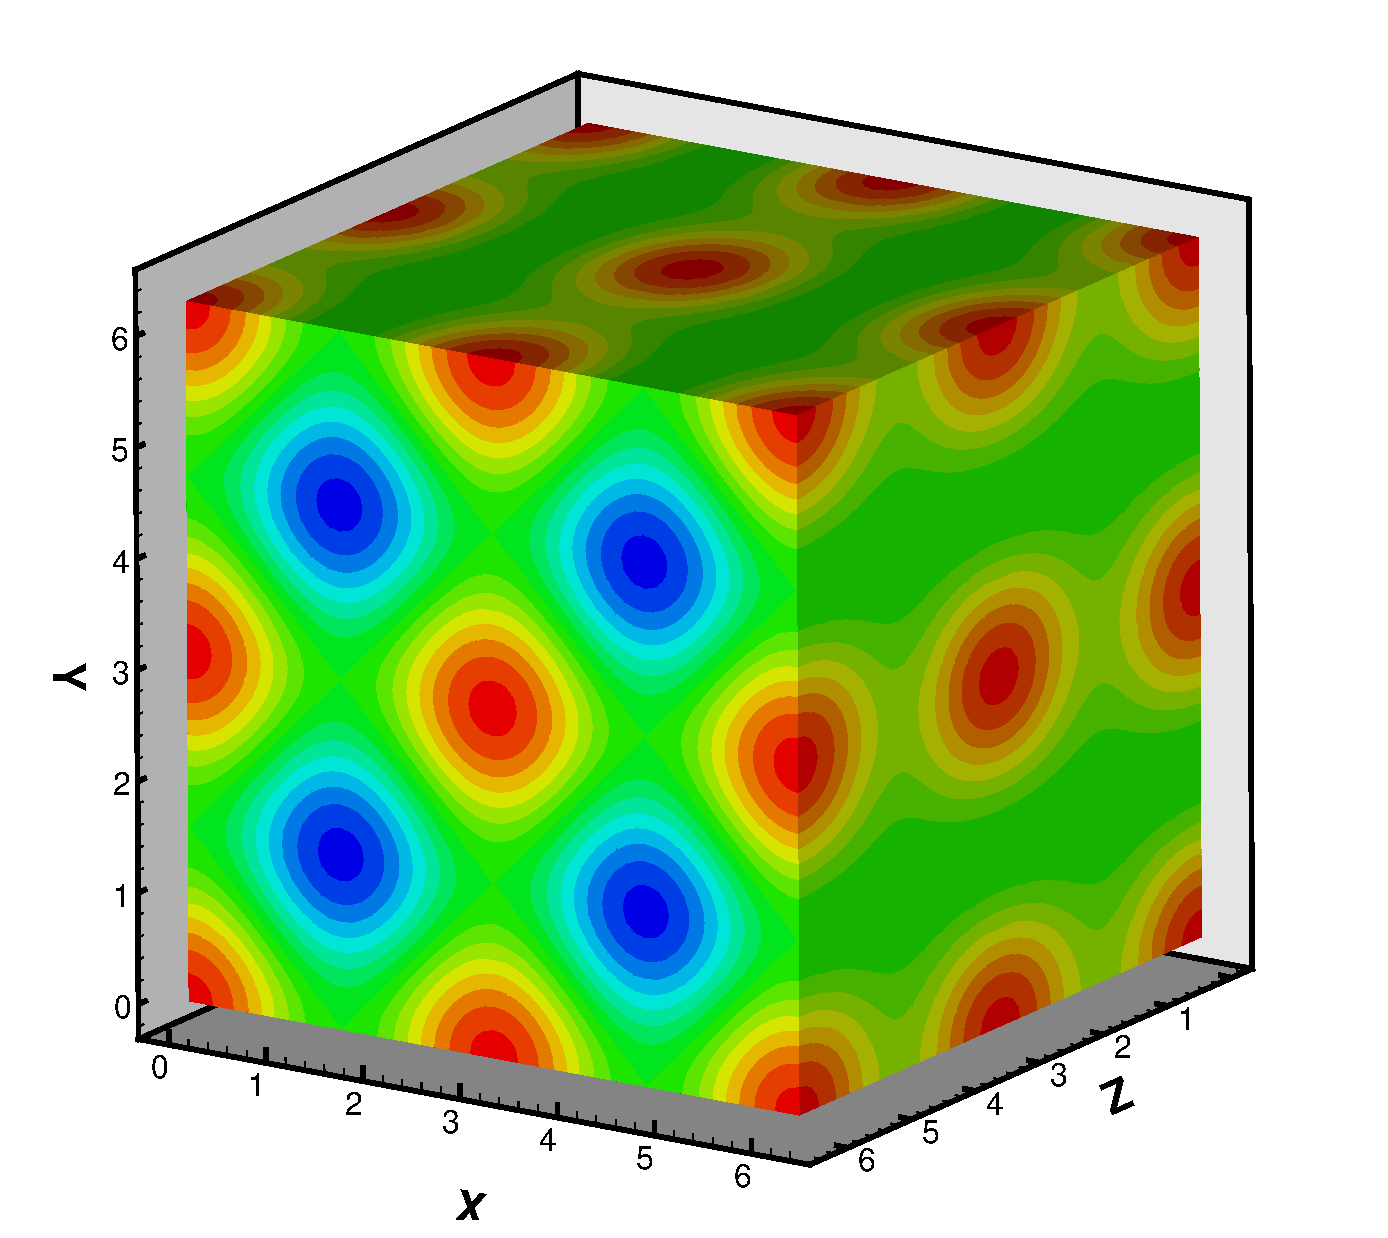
\includegraphics[scale=0.45]{Figures/06-01-pressure.eps}}
  \end{picture}
  \caption{Pressure field prescribed by Eq.~\ref{eq_pressure_init}}
  \label{fig_pressure}
\end{figure}

%---------------------------------------------------------------------nutshell-%
\vspace*{5mm} \fbox{ \begin{minipage}[c] {0.97\textwidth} %-----------nutshell-%
    {\sf Section \ref{sec_scalars} in a nutshell} \\  %---------------nutshell-%
   
      - Scalar fields are defined with {\psiboil} class {\tt Scalar}. \\

      - {\tt Scalar} is defined for a {\tt Domain}, with the constructor:
      \begin{itemize}
        \item {\tt Scalar(Domain \&);}
      \end{itemize}
 
      - {\tt Scalar}'s values are accessed with the usual {\tt C++} syntax:
      \begin{itemize}
        \item {\tt p[i][j][k];}
      \end{itemize}

      - To browse through all the {\tt Scalar} values, use the following macro:
      \begin{itemize}
        \item {\tt for\_vijk(Scalar \&, int i, int j, int k);}
      \end{itemize}
       Similar macros are defined in directory: {\tt PSI-Boil/Src/Field/Scalar/scalar\_browsing}. \\

      - {\tt Scalar} has a number of member functions to access {\tt Domain}s
      geometrical quantities. 
    
  \end{minipage} } %--------------------------------------------------nutshell-%
%---------------------------------------------------------------------nutshell-%

  \section{Vectors}
\label{sec_vectors}

Example program which defines vector field {\tt uvw}, assigns initial
values to it, and plots it, is given below:
%
{\small \begin{verbatim}
     ...
     20   /* define unknowns */
     21   Vector uvw(d); // velocity
     22
     23   /* assign initial values to velocity in "i" direction */
     24   Comp m = Comp::u();
     25   for_vmijk(uvw,m,i,j,k)
     26     uvw[m][i][j][k] =  sin(uvw.xc(m,i)) * cos(uvw.yc(m,j)) * cos(uvw.zc(m,k));
     27
     28   /* assign initial values to velocity in "j" direction */
     29   Comp m = Comp::v();
     30   for_vmijk(uvw,m,i,j,k)
     31     uvw[m][i][j][k] = -cos(uvw.xc(m,i)) * sin(uvw.yc(m,j)) * cos(uvw.zc(m,k));
     32
     33   /* plot vector */
     34   boil::plot->plot(uvw, "velocity", 0);
     ...
\end{verbatim}}
%
Only the lines which are different to program {\tt 06-01-main.cpp} are given. This
program is stored as {\tt 06-03-main.cpp}. Velocity vector {\tt uvw} is created 
from computational domain only in line~21, as an object of type {\tt Vector}.

Vector field {\tt uvw} stores three Cartesian velocity components: $u$,
$v$ and $w$. The program actually initializes {\tt uvw} to:
%
\bea
  u & = &  sin(x) cos(y) cos(z) \\
  v & = & -cos(x) sin(y) cos(z) \\
  w & = & 0
  \label{eq_velocity}
\eea
%
Observe in lines~26 and~31 that {\tt Vector} fields are accessed like the 
four-dimensional matrices in {\tt C++}: {\tt uvw[m][i][j][k];}, where {\tt m} is 
a component counter ({\tt Comp::u()} for $u$, {\tt Comp::v()} for $v$ and 
{\tt Comp::w()} for $w$), and {\tt i}, {\tt j} 
and {\tt k} are positions in three-dimensional structured domain. 

For shorter and safer browsing through vectors, a number of macros have been
defined in {\tt Vector/vector\_browsing.h}, in a similar way it was done
for scalar. Two examples are given in above
listing, in lines~25 and~30. The macro:
%
{\small \begin{verbatim}
     30   for_vmijk(uvw,m,i,j,k)
\end{verbatim}}
%
takes as parameters the {\tt Vector} field ({\tt uvw}), the component for
which you want to browse ({\tt m}), and counters in $i$, $j$ and $k$ 
direction ({\tt i}, {\tt j} and {\tt k}.

One might wonder at this point why do we have to send vector component ({\tt m})
to macro for browsing, isn't the grid defined by {\tt Vector}'s member functions
{\tt si()}, {\tt ei()}, {\tt sj()}, \ldots. Well, it must not be forgotten that
vectors are defined on a staggered grid, which means their resolution is different
from {\tt Scalar}'s, and, even more, it is different for each vector component.

Make a small test. Insert the following lines to program~{\tt 06-03-main.cpp}:
%
{\small \begin{verbatim}
     33   /* resolution of "u" velocity component */
     34   OPR(uvw.ni( Comp::u() ));
     35   OPR(uvw.nj( Comp::u() ));
     36   OPR(uvw.nk( Comp::u() ));
     37   /* resolution of "v" velocity component */
     38   OPR(uvw.ni( Comp::v() ));
     39   OPR(uvw.nj( Comp::v() ));
     40   OPR(uvw.nk( Comp::v() ));
     41   /* resolution of "w" velocity component */
     42   OPR(uvw.ni( Comp::w() ));
     43   OPR(uvw.nj( Comp::w() ));
     44   OPR(uvw.nk( Comp::w() ));
\end{verbatim}}
%
Re-compile and re-run to get:
%
{\small \begin{verbatim}
FILE: main.cpp, LINE: 34, uvw.ni( Comp::u() ) = 67
FILE: main.cpp, LINE: 35, uvw.nj( Comp::u() ) = 66
FILE: main.cpp, LINE: 36, uvw.nk( Comp::u() ) = 66
FILE: main.cpp, LINE: 38, uvw.ni( Comp::v() ) = 66
FILE: main.cpp, LINE: 39, uvw.nj( Comp::v() ) = 67
FILE: main.cpp, LINE: 40, uvw.nk( Comp::v() ) = 66
FILE: main.cpp, LINE: 42, uvw.ni( Comp::w() ) = 66
FILE: main.cpp, LINE: 43, uvw.nj( Comp::w() ) = 66
FILE: main.cpp, LINE: 44, uvw.nk( Comp::w() ) = 67
\end{verbatim}}
%
Apparently, resolution is different for each vector component. The reason is
easy to understand. As the grid in shifted\footnote{staggered} in $i$ direction, 
additional cells are created on the plane of faces at the beginning of the domain. 
The same holds for shifts in $j$ and $k$ direction, with increase in according
directions.
The increase of number of cells due to staggering is illustrated 
in Fig.~\ref{fig_staggering}.
%
%--------------%
%              %
%  Staggering  %
%              %
%--------------%
\begin{figure}[ht]
  \centering
  \setlength{\unitlength}{1mm}
  \begin{picture}(100,50)(0,0)
    \thickbox{100}{50}
    \put(0,0){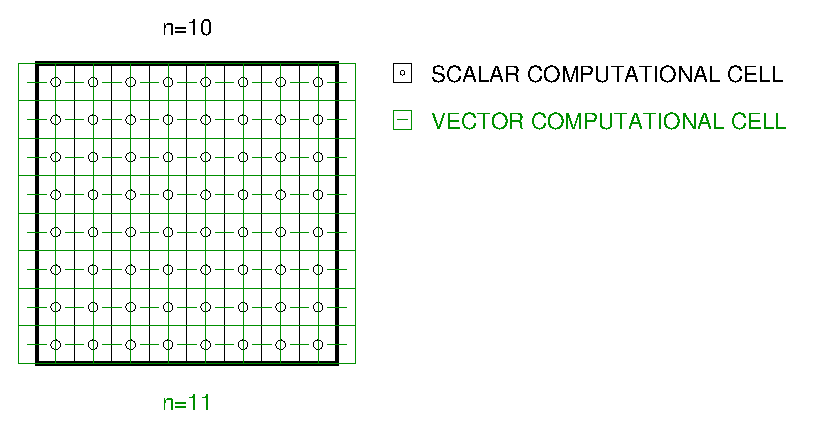
\includegraphics[scale=0.75]{Figures/06-02-staggering.eps}}
  \end{picture}
  \caption{Number of cell rows for a {\tt Vector} field is greater by
           one  than than for {\tt Scalar} field, in the direction
           of staggering.}
  \label{fig_staggering}
\end{figure}
%
For the same reason, many {\tt Vector}'s member functions related to geometrical 
quantities (such as {\tt dxc()}, {\tt dyc()}, {\tt dzc()}, {\tt dxw()}, {\tt dxe()},
{\tt dV()}, \ldots) also depend on {\tt Vector}'s component.

Velocity field prescribed by program ({\tt 06-03-main.cpp}) is shown in
Fig.~\ref{fig_velocity}.
 
%------------%
%            %
%  Velocity  %
%            %
%------------%
\begin{figure}[ht]
  \centering
  \setlength{\unitlength}{1mm}
  \begin{picture}(100,85)(0,0)
    \thickbox{100}{85}
    \put(0,-3){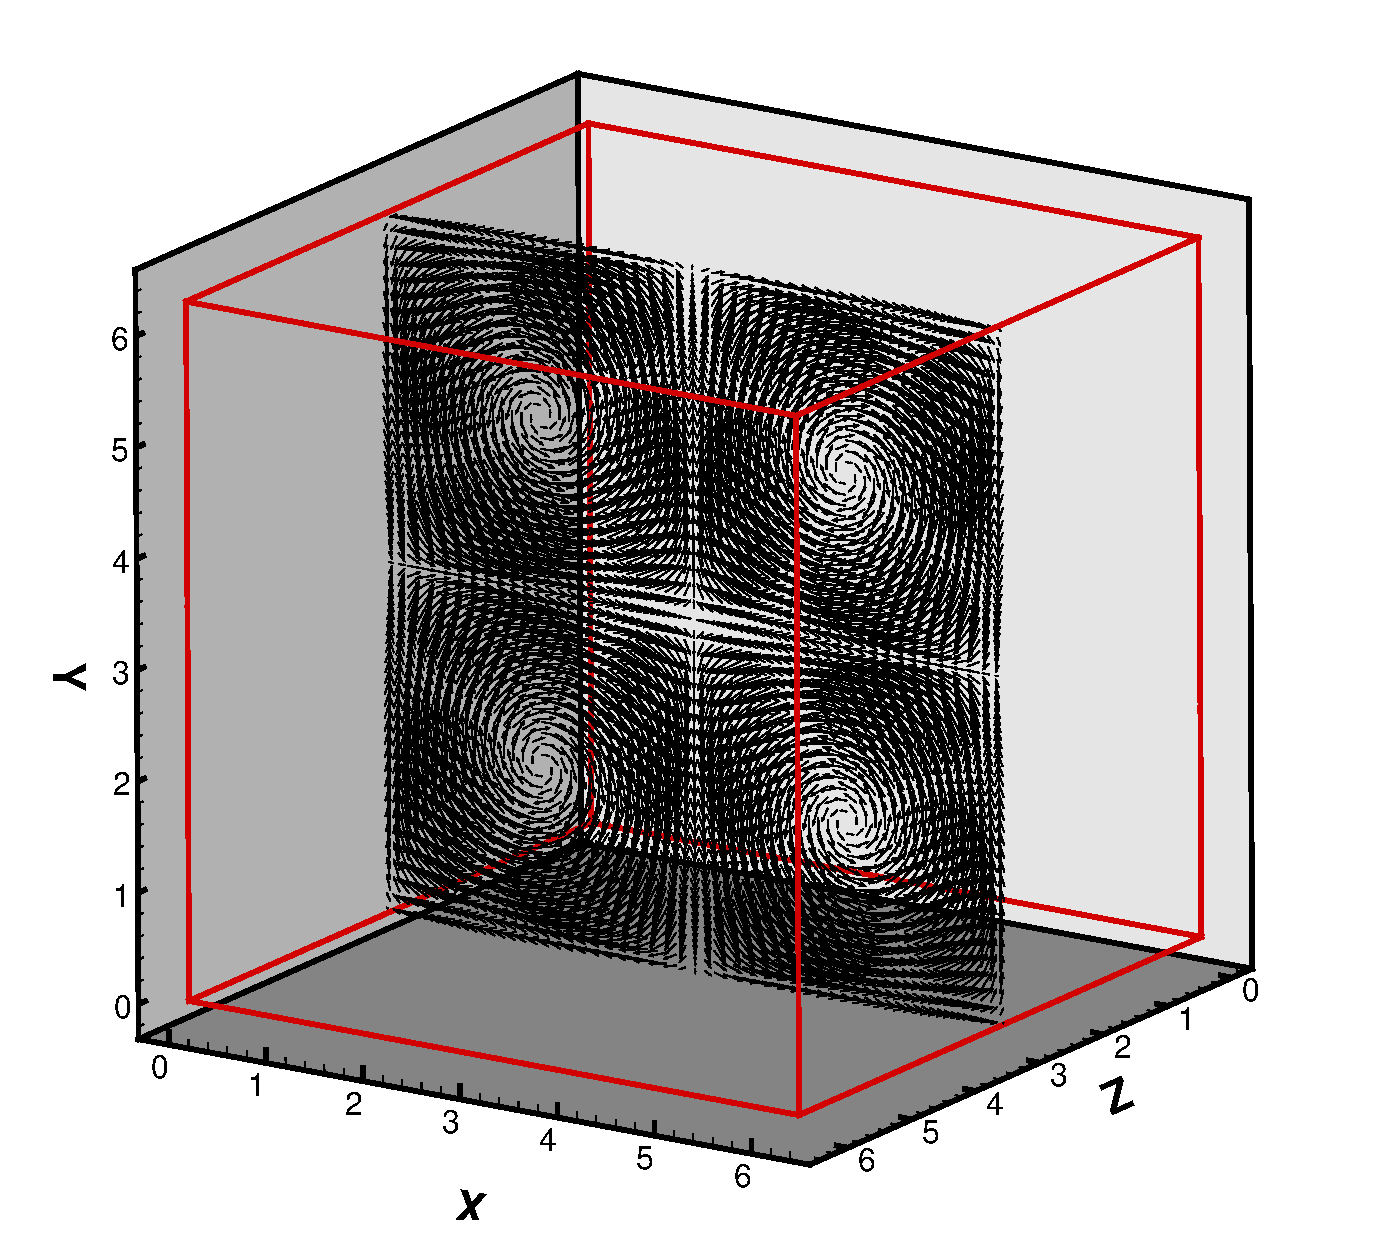
\includegraphics[scale=0.45]{Figures/06-03-velocity.eps}}
  \end{picture}
  \caption{Pressure field prescribed by Eq.~\ref{eq_velocity}}
  \label{fig_velocity}
\end{figure}

\clearpage

%---------------------------------------------------------------------nutshell-%
\vspace*{5mm} \fbox{ \begin{minipage}[c] {0.97\textwidth} %-----------nutshell-%
    {\sf Section \ref{sec_vectors} in a nutshell} \\  %---------------nutshell-%
   
      - Vector fields are defined with {\psiboil} class {\tt Vector}. \\

      - {\tt Vector} is defined for a {\tt Domain}, with the constructor:
      \begin{itemize}
        \item {\tt Vector(Domain \&);}
      \end{itemize}
 
      - {\tt Vector}'s values are accessed with the usual {\tt C++} syntax:
      \begin{itemize}
        \item {\tt p[m][i][j][k];}
      \end{itemize}
      where {\tt m} is a vector component ranging from 0-3 (for $i$, $j$ and $k$). \\

      - To browse through all the {\tt Vector} values of component {\tt m}, 
      use the following macro:
      \begin{itemize}
        \item {\tt for\_vmijk(Vector \&, int m, int i, int j, int k);}
      \end{itemize}
       Similar macros are defined in directory: {\tt PSI-Boil/Src/Vector/vector\_browsing}. \\

      - {\tt Vector} has a number of member functions to access {\tt Domain}s
      geometrical quantities. Most of them depend on the {\tt Vector}'s component
    
  \end{minipage} } %--------------------------------------------------nutshell-%
%---------------------------------------------------------------------nutshell-%


  %-----------%
  %           %
  %  Solvers  %
  %           %
  %-----------%
  \chapter{Transport Equation Solvers}
  \label{chap_single_phase}

This chapter deals with the solution of transport equation for incompressible
fluid flow. The equation which describes this phenomenon is momentum
conservation equation, given by~\ref{eq_momentum}, repeated here for
convenience:
%
\be
         \int_V \frac{\p \rho \uvw}{\p t} dV
       + \int_S \rho \uvw \uvw \, dS
       = \int_S \mu \nabla \uvw \, dS
       - \int_V \nabla p \, dV
       + {\bf F}
       \; \; \; \;
       [N]
  \label{eq_momentum_2}
\ee
%
This form, however,
poses a problem. We have one three equations (one for each velocity 
component), but for unknowns: velocity components and pressure. 

For incompressible flow problems, pressure has always been sought through
additional constraint, mass conservation equation:
%
\be
       \int_V \frac{\p \rho}{\p t} dV 
       = 
       - \int_S \rho \uvw d{\bf S}
       \; \; \; \;
       [\frac{kg}{s}]
  \label{eq_mass}
\ee
% 
Momentum and mass conservation have been linked in various ways, providing
different algorithms for computation of incompressible flows. The most
widely used in applied CFD are SIMPLE, SIMPLEC, SIMPLER and even PISO 
({\bf references}). For highly unsteady flow, at simulation of which
{\psiboil} aims, the most efficient is the {\em fractional step method},
sometimes referred to as the {\em projection} method. It combines momentum
conservation equation~(\ref{eq_momentum}) with mass conservation
equation~(\ref{eq_mass}), at intermediate time between two simulated
time steps, to give additional equation for pressure (already introduced
as~\ref{eq_pressure}):
%
\be
         \int_S \frac{\nabla p}{\rho} \, d{\bf S} 
       = \frac{1}{\Delta t} \int_S \uvw^\s \, d{\bf S}
       \; \; \; \; 
       [ \frac{m^3}{s^2} ],
  \label{eq_pressure_2}
\ee
%
often referred to as pressure-Poisson equation.

The fractional step method, which is used by {\psiboil}, is now outlined.
The momentum conservation equation~(\ref{eq_momentum_2}) must first be discretized
in time, part by part. The most usual approach is to use Crank-Nicolson
scheme for diffusion (to avoid very low time steps needed by the forward
Euler scheme) and to use Adams-Bashforth for convection, for the sake
of simplicity. Inertial terms are discretized with backward Euler scheme.
The time-discretized momentum equation then looks like:
%
\be
        {\bf I}^\s - {\bf I}^{n-1} 
       + \frac{3}{2} {\bf C}^{n-1} - \frac{1}{2} {\bf C}^{n-2}
       = \frac{1}{2} {\bf D}^\s + \frac{1}{2} {\bf D}^{n-1}
       + {\bf F}^{n-1}
  \label{eq_semi}
\ee
%
Here, $\s$ denotes the tentative (intermediate) time step, while 
${\bf I}^\s = \frac{1}{\Delta t} \int_V  \rho \uvw^\s dV$ 
and ${\bf D}^\s = \int_S \mu \nabla \uvw^\s \, d{\bf S}$ 
denote inertial and diffusive term in the tentative time step. 
Old (known) values of velocity (at time step $n-1$) define terms:
${\bf I}^{n-1} = \frac{1}{\Delta t} \int_V  \rho \uvw^{n-1} dV$,
and ${\bf D}^{n-1} = \int_S \mu \nabla \uvw^{n-1} \, d{\bf S}$, as well
as convective term at old time step: 
${\bf C}^{n-1} = \int_S \rho \uvw^{n-1}\uvw^{n-1} \, d{\bf S}$. Clearly,
${\bf C}^{n-2} = \int_S \rho \uvw^{n-2}\uvw^{n-2} \, d{\bf S}$.

Equation~\ref{eq_semi} is discretized in space giving a linear system
of equations for intermediate velocity~($\uvw^\s$). Once this
system is solved gives velocity field which does not, generally, 
satisfies mass conservation equation. It is used to compute pressure 
from~\ref{eq_pressure_2}. The computed pressure is used to {\em project}
velocity into a divergence free velocity field:
%
\be
  \uvw^{n} = \uvw^\s + \frac{1}{\rho} \nabla p \, \Delta t
  \label{eq_projection}
\ee
%
which represents velocity at new time step. 

% wrong: {\psiboil} uses only fractional step method to link velocity and pressure.
% wrong: This also means that {\psiboil} can be used to simulate only unsteady 
% wrong: phenomena. If steady solution is sought, the governing equations should
% wrong: be integrated long enough until steady state is reached.

  
  \section{Transport equations in {\psiboil}}
\label{sec_equations}

In this section, transport equations currently implemented in {\psiboil} 
are briefly outlined. They all written in {\em conservative} form
because it is closer to physical laws we are trying to simulate and 
because the FV method employed by {\psiboil} discretizes transport
equations in the same form. Furthermore, physical units for
each equation are given, since it serves as a good check whether the
implementation (discretization) of each member in the equation is 
valid. 

\subsection{Species conservation equation}

Species conservation equations, defined with the class {\tt Concentration}, reads:
%
\be
         \int_V \frac{\p \rho \alpha}{\p t} dV
       + \int_S \rho \uvw \alpha \, d{\bf S}
       = \int_S \gamma \nabla \alpha \, d{\bf S}
       + \dot{M}
       \; \; \; \;
       [\frac{kg}{s}]
  \label{eq_species}
\ee
%
where $\rho \; [\frac{kg}{m^3}]$ is the mass density, $\alpha \; [1]$ is the
species concentration, $t \; [s]$ is time, $\uvw \; [\frac{m}{s}]$ is velocity 
field, $\gamma \; [\frac{kg}{ms}]$, and $\dot{M} \; [\frac{kg}{s}]$ is the 
species source. The equation is written in integral form, i.e.\ it is defined
for a general volume $V \; [m^3]$, enclosed by surface $S \; [m^2]$.

Class {\tt Concentration} is derived from {\tt Centered}, which is a derivation
of {\tt Equation}. {\tt Concentration} is defined in 
{\tt PSI-Boil/Src/Equation/Centered/Concentration}.

\subsection{Enthalpy conservation equation}

Enthalpy conservation equations, defined with the class {\tt Enthalpy}, reads:
%
\be
         \int_V \frac{\p \rho C_p T}{\p t} dV
       + \int_S \rho C_p \uvw T \, d{\bf S}
       = \int_S \lambda \nabla T \, d{\bf S}
       + \dot{Q}
       \; \; \; \;
       [\frac{J}{s} = W]
  \label{eq_enthalpy}
\ee
%
where $C_p \; [\frac{J}{kg \, K}]$ is thermal capacity, $T \; [K]$ is the 
temperature, $\lambda \; [\frac{W}{m \, K}]$ the heat conductivity and 
$\dot{Q} \; [\frac{J}{s}]$ is the heat source.

{\tt Enthalpy} is defined in {\tt PSI-Boil/Src/Equation/Centered/Enthalpy}
and is derived from {\tt Centered} and {\tt Equation}.

\subsection{Phase indicator equation}

Phase indicator function ($\Phi$), defined in the class {\tt LevelSet}, is used
in conjunction with conservative Level-Set (LS) method implemented in
{\psiboil}. Essentially, it is purely hyperbolic conservation equation for~$\Phi$:
%
\be
         \int_V \frac{\p \Phi}{\p t} dV
       + \int_S \uvw \Phi \, d{\bf S}
       = 
       0
       \; \; \; \;
       [\frac{m^3}{s}]
\ee

Class {\tt LevelSet} is defined in {\tt PSI-Boil/Src/Equation/Centered/LevelSet}
and has the same ancestry as {\tt Enthalpy} and {\tt Concentration}. {\tt LevelSet}
may be a bit of a misnomer, so it might change it's name in the future.

\subsection{Pressure-Poisson equation}

Not really a transported quantity, but result of the time discretization of
momentum conservation equations, pressure-Poisson equation is defined as:
%
\be
         \int_S \frac{\nabla p'}{\rho} \, d{\bf S} 
       = \frac{1}{\Delta t} \int_S \uvw \, d{\bf S}
       \; \; \; \; 
       [ \frac{m^3}{s^2} ],
  \label{eq_pressure}
\ee
% 
where $p \; [\frac{kg}{m \, s^2} = Pa]$ is the pressure. As all the other
cell-centered {\tt Equation}s, {\tt Pressure} is derived from {\tt Centered}
and {\tt Equation}. It's definition can be found in:
{\tt PSI-Boil/Src/Equation/Centered/Pressure}.

\subsection{Momentum conservation equation}

The only class belonging to {\tt Staggered} branch of {\tt Equation}s,
is the {\tt Momentum}, which discretizes the momentum conservation 
equation:
%
\be
         \int_V \frac{\p \rho \uvw}{\p t} dV
       + \int_S \rho \uvw \uvw \, dS
       = \int_S \mu \nabla \uvw \, dS
       - \int_V \nabla p \, dV
       + {\bf F}
       \; \; \; \;
       [\frac{kg \, m}{s^2} = N]
  \label{eq_momentum}
\ee
%
Here, $\mu \; [\frac{kg}{m \, s}]$ is dynamic viscosity. 

{\tt Momentum} is the only class derived from {\tt Staggered}, which is
derived from {\tt Equation}. Class {\tt Momentum} is defined in:
{\tt PSI-Boil/Src/Equation/Staggered/Momentum}.

%---------------------------------------------------------------------nutshell-%
\vspace*{5mm} \fbox{ \begin{minipage}[c] {0.97\textwidth} %-----------nutshell-%
    {\sf Section \ref{sec_equations} in a nutshell} \\  %-------------nutshell-%
   
      - Transport equations in {\psiboil} are defined as the class {\tt Equation}
      serving as a parent to: 
      \begin{itemize}
        \item {\tt Centered} for cell-centered variables, spawning to 
        \begin{itemize}
           \item {\tt Concentration} - species conservation equation,
           \item {\tt Enthalpy}     - enthalpy conservation equation,
           \item {\tt LevelSet}     - phase indicator equation for LS method,
           \item {\tt Pressure}     - pressure-Poisson equation,
        \end{itemize}
        \item and {\tt Staggered} for face-centered (staggered) variables, 
              used only as a parent to
        \begin{itemize}
           \item {\tt Momentum} - momentum conservation equation.
        \end{itemize}
      \end{itemize}

  \end{minipage} } %--------------------------------------------------nutshell-%
%---------------------------------------------------------------------nutshell-%
  
  \section{Simulation of heat conduction}
\label{sec_conduction}

Having briefly introduced transport {\tt Equation}s in {\psiboil} we move
forward to apply one of them to solve a simple steady heat conduction 
problem, governed by the equation:
%
\be
         \int_S \lambda \nabla T \, d{\bf S}
       = 0           
       \; \; \; \;
       [W]
  \label{eq_conduction}
\ee
%
It is clearly a special case of Eq.~\ref{eq_enthalpy}, without unsteady,
convective and source terms.

Let's consider a cubical computational domain, having dimensions 
$1 \times 1 \times 1$, and let's impose the following boundary conditions:
%
\begin{itemize}
  \item $T = 300 \; [K]$ at $x = 0$
  \item $T = 400 \; [K]$ at $x = 1$
  \item $\frac{\p T}{\p n} = 0$ everywhere else
\end{itemize}

The program which discretizes and solves this problem follows ({\tt 07-01-main.cpp}):
%
{\small \begin{verbatim}
      1 #include "Include/psi-boil.h"
      2
      3 const real L =  1.0;
      4 const int  N = 64;
      5
      6 /****************************************************************************/
      7 main(int argc, char * argv[]) {
      8
      9   boil::timer.start();
     10
     11   Grid1D g( Range<real>(0,L), N, Periodic::no());
     12   Domain d(g, g, g);
     13
     14   Scalar t(d), q(d);                          /* temperature and its source */
     15   Vector uvw(d);                              /* velocity field */
     16
     17   t.bc().add( BndCnd( Dir::imin(), BndType::dirichlet(), 300.0 ) ); /* b.c. */
     18   t.bc().add( BndCnd( Dir::imax(), BndType::dirichlet(), 400.0 ) ); /* b.c. */
     19   t.bc().add( BndCnd( Dir::jmin(), BndType::neumann() ) );          /* b.c. */
     20   t.bc().add( BndCnd( Dir::jmax(), BndType::neumann() ) );          /* b.c. */
     21   t.bc().add( BndCnd( Dir::kmin(), BndType::neumann() ) );          /* b.c. */
     22   t.bc().add( BndCnd( Dir::kmax(), BndType::neumann() ) );          /* b.c. */
     23
     24   Matter solid(d);                                  /* matter */
     25
     26   Krylov * solver = new CG(d, Prec::di());          /* linear solver */
     27
     28   Times time;                                       /* simulation time */
     29
     30   Enthalpy enth(t, q, uvw, time, solver, &solid);   /* enthalpy conservation
     31                                                        equation              */
     32   enth.diffusion_set(TimeScheme::backward_euler()); /* time stepping scheme */
     33
     34   AC multigrid( &enth );                            /* AMG solver for enth. */
     35
     36   t = 350.0;                                        /* initial "guess" */
     37
     38   multigrid.vcycle(ResRat(1e-4));                   /* solve linear system */
     39
     40   boil::plot = new PlotTEC();
     41   boil::plot->plot(t, "t");
     42
     43   boil::timer.stop();
     44   boil::timer.report();
     45 }
\end{verbatim}}
%
Although the problem being solved is simple, the program {\tt 07-01-main.cpp}
introduces many new concepts and each of them is presented in a separate subsection. 

\subsection{Boundary conditions}
\label{sub_sec_bc}

Boundary conditions are defined for fields, i.e.\ for {\tt Scalar}s and
for {\tt Vector}s. A class {\tt BndCnd}, defined in {\tt Src/Boundary}
holds the boundary conditions for various fields. {\tt BndCnd} can be 
defined in several ways (you can find them all in {\tt Src/Boundary/bndcnd.h},
but essentially, it is defined by {\em direction}, boundary condition {\em type} 
and {\em value}.

\subsubsection{Direction}

First parameter to define a boundary condition is {\em direction}. 
Direction can denote any of the logical six boundaries of computational 
{\tt Domain}, meaning: $i_{min}$ and $i_{max}$ (sometimes also referred 
to as {\em west} and {\em east}), $j_{min}$ and $j_{max}$ (or {\em south} 
and {\em north}), and $k_{min}$ and $k_{max}$ (or {\em bottom} and {\em top}). 
These directions are represented with ravioli object {\tt Dir}, which can 
assume one of the following values\footnote{Actually, {\tt Dir} is used as
if it was a constant defining direction. But a constant which is easy
to understand and for which compiler performs checking, when passed as
an argument}:
%
\begin{itemize}
  \item {\tt Dir::imin();} - west,
  \item {\tt Dir::imax();} - east,
  \item {\tt Dir::jmin();} - south,
  \item {\tt Dir::jmax();} - north,
  \item {\tt Dir::kmin();} - bottom and
  \item {\tt Dir::kmax();} - north boundary of the {\tt Domain}.
\end{itemize}
%
{\tt Dir} is a ravioli object and is defined in {\tt Src/Ravioli}.

\subsubsection{Boundary condition type}

Boundary condition type is stored in the ravioli class {\tt BndType} which,
since used only with {\tt BndCnd} is not defined in {\tt Src/Ravioli}
directory, but together with {\tt BndCnd}, in {\tt Src/Boundary}. 
{\tt BndType}, can assume one of the following values:
%
\begin{itemize}
  \item {\tt BndType::undefined();} 
  \item {\tt BndType::dirichlet();}
  \item {\tt BndType::neumann();}
  \item {\tt BndType::periodic();}
  \item {\tt BndType::inlet();}
  \item {\tt BndType::outlet();}
  \item {\tt BndType::wall();}
  \item {\tt BndType::symmetry();}
\end{itemize}
%
which are self-explanatory. ({\bf Check later if all {\tt BndType}s are 
applicable to all {\tt Equation}s})

\subsubsection{Boundary condition value}

This argument is optional. Namely, for some boundary conditions, such as 
symmetry and periodic, it does not have to be specified. If value is not
for other {\tt BndType}s, it is assumed to be equal to zero.
%
Value can be specified as a {\tt real} number, but also analytically,
as a function of $x$, $y$ and $z$ coordinates. That will be covered in
later sections. 

\subsubsection{Final form of boundary condition definition}

For example, to define a {\em Dirichlet} boundary condition at the 
{\em west} boundary of the {\tt Domain} (at $i = i_{min}$), with the
value of~300, we use the line:
%
{\small \begin{verbatim}
     BndCnd( Dir::imin(), BndType::dirichlet(), 300.0 );
\end{verbatim}}
%
To define a {\em Neumann} condition at the {\em north} boundary~($j = j_{max}$),
we do not have to specify the value, so the syntax is:
%
{\small \begin{verbatim}
     BndCnd( Dir::jmax(), BndType::neumann() );
\end{verbatim}}
%
These definitions are pointless if not assigned to fields representing
transported quantities. To achieve that, we use the member function: 
%
{\small \begin{verbatim}
     Scalar::bc().add( BndCnd & );
\end{verbatim}}
%
Program lines~17--22 assign various boundary conditions to {\tt Scalar t}.
The lines look cramped a bit, but that is because boundary condition 
object ({\tt BndCnd}) is defined at the place it is also passed as 
argument to {\tt Scalar::bc().add()}. To illustrate it further, program line~17,
with all the parts clearly denoted is shown below:
%
\bea
{\tt t.bc().add(} \; \overbrace{
              {\tt BndCnd(} 
                \overbrace{
                  \;
                  \underbrace{ {\tt Dir::imin()} }_{ \mbox{direction} }
                  , \;
                  \underbrace{ \; {\tt BndType::dirichlet()} }_{ \mbox{b.c.\ type} }
                  , \;
                  \underbrace{ \; {\tt 300.0} }_{ \mbox{value} }
                  \;
                }^{ \mbox{arguments to {\tt BndCnd(,,)}}} 
              )
            }^{ \mbox{{\tt BndCnd} is argument to {\tt add()}} } 
          \; 
{\tt );} \nonumber
\eea

\subsection{Matter}

There is a new
type of object defined in line~24, called {\tt Matter}. For every {\tt Equation}
solved by {\psiboil}, {\tt Matter} must be defined, bringing with it a suite of
physical properties featured in governing equations presented in Sec.~\ref{sec_equations}.
For this example, governed by the equation for steady conduction (Eq.~\ref{eq_conduction}
no property needs to be adjusted. Furthermore, {\tt Matter} can be defined as a
{\em mixture}, but that will not be covered in this section. Therefore, we simply
define an object of type {\tt Matter} now. 

\subsection{Krylov}

Next novelty is the object of type {\tt Krylov}, which is a linear solver
used to solve systems of discretized equations, created in line~26. Currently,
there are three solvers from Krylov sub-space family defined: Conjugate Gradient
(implemented as {\tt CG}), Bi-Conjugate Gradient~(as {\tt BiCG}) and Conjugate 
Gradient Squared~(implemented as class {\tt CGS}). 
{\tt Krylov} is a parent class to these three 
solvers and as such, it can {\em point} to each of them\footnote{Remember that
pointer to a parent class is also a pointer to all of it's children.}. A 
particular solver can be selected from one of the following constructors:

\begin{itemize}
  \item {\tt Krylov * solver = new CG  (d, Prec::di());} for CG   solver
  \item {\tt Krylov * solver = new BiCG(d, Prec::di());} for BiCG solver
  \item {\tt Krylov * solver = new CGS (d, Prec::di());} for CGS  solver
\end{itemize}

Constructor to each of the solvers takes a {\tt Domain} as first argument
and type of {\em preconditioner} as a second. Type of preconditioner is
defined by a ravioli object {\tt Preconditioner} and it can assume one of
the following values\footnote{This ravioli object is not defined in directory
{\tt Src/Ravioli}, because it is used only with {\tt Krylov} type solvers.}:
%
\begin{itemize}
  \item {\tt Preconditioner::di()} for diagonal,  
  \item {\tt Preconditioner::ic()} for Incomplete Cholesky, and  
  \item {\tt Preconditioner::no()} for no preconditioning.           
\end{itemize}

\subsection{Times}

Object of type {\tt Times} is defined in line~28. It defines the simulation
time, i.e.\ number of time steps which have to be performed, and a value
for the time step. In present case, which is steady\footnote{Steady cases are
an exception for kind of problems {\psiboil} aims at}, nothing needs to
be specified. 
{\tt Times} is a ravioli type object, defined in directory {\tt Src/Ravioli}. 
It is also useful in time-integration loops for unsteady problems, as will 
be shown below. 

\subsection{Transport equation}

Once we have field for transported quantity (here the temperature, {\tt Scalar t}), 
field for it's source (here {\tt Scalar q}), convective velocity field 
({\tt Vector uvw}), simulation time ({\tt Times time}) and a linear solver
({\tt Krylov * solver}), we can define a transport equation with the
constructor:
%
{\small \begin{verbatim}
     30   Enthalpy enth(t, q, uvw, time, solver, &solid); 
\end{verbatim}}
% 
Convective velocity field, source and time, {\em must} be provided, no matter
if problem involves transport by velocity, has any external sources, or is it
unsteady. It may look as an overhead, but keep in mind that {\em vast} majority 
of problems analyzed with {\psiboil} are {\em unsteady}, involve fluid flow 
and feature external {\em sources} on transported variables. Actually, it would
be an overhead to write additional constructors for these special cases which
occur very rarely. 
%
The form of constructor shown above is {\em the same} for all transport 
{\tt Equation}s implemented in {\psiboil}. Constructor for {\tt Equation},
such as the one in line~30, also discretizes the governing transport
equation, for this case, it is the enthalpy conservation defined 
with~Eq.~\ref{eq_enthalpy}.

\subsection{Time-stepping scheme}
\label{sub_sec_time_stepping}

For each transport equation, time stepping scheme can be set for {\em diffusive}
and {\em convective} terms. If nothing is specified, {\psiboil} uses  
default schemes, which are:
%
\begin{itemize}
  \item {\em Adams-Bashforth} for convection, and
  \item {\em Crank-Nicolson} for diffusive terms. 
\end{itemize}
%
For steady cases\footnote{Again: which is an exception}, time stepping 
scheme should be set to {\em steady}.
%
In this case, there is no convection, so setting the time-stepping scheme 
for convection is pointless. For diffusion, it is set with the line:
%
{\small \begin{verbatim}
     32   enth.diffusion_set(TimeScheme::steady()); 
\end{verbatim}}
% 
This setting uses {\tt Equation}'s member function {\tt diffusion\_set}
and ravioli object {\tt TimeScheme}, which can have one of the following
values:
%
\begin{itemize}
  \item {\tt TimeScheme::backward\_euler();} 
  \item {\tt TimeScheme::crank\_nicolson();}
  \item {\tt TimeScheme::adams\_bashforth();}
\end{itemize}
%

\subsection{Additive correction multigrid solver}

This case, since steady, results in relatively poorly conditioned linear
system of discretized equations. Therefore, it is sound to use a multigrid
procedure to accelerate it's convergence. {\psiboil} has only one multigrid
algorithm, based on Additive Correction (AC) scheme ({\bf add reference}). It
is defined in class~{\tt AC}. Algebraic multigrid is based on coarsening
discretized system of equations and solving these coarser (smaller) systems
faster, leading to faster reduction of residuals on finer (bigger) levels
as well. {\tt AC} is defined in line~34:
%
{\small \begin{verbatim}
     34   AC multigrid( &enth );  
\end{verbatim}}
% 
It takes the reference to {\tt Equation} as a parameter. Remember that
{\tt Equation} was already defined with a linear solver ({\tt solver}),
which will be used by {\tt AC} to {\em smooth} each refinement level. 

The solution of the liner system by {\tt AC} is invoked by:
%
{\small \begin{verbatim}
     38   multigrid.vcycle(ResRat(1e-4));
\end{verbatim}}
% 
which starts a "V" multigrid cycle and runs until residuals fall four
levels of magnitude. 

This program creates the following output:
%
{\small \begin{verbatim}
Domain level 4 created !
Domain level 3 created !
Domain level 2 created !
Domain level 1 created !
FILE: centered_coarsen.cpp, LINE: 6, coarsenig
Centered level 32 x 32 x 32 created !
Centered level 16 x 16 x 16 created !
Centered level 8 x 8 x 8 created !
Centered level 4 x 4 x 4 created !
Number of cycling levels: 5
FILE: centered_update_rhs.cpp, LINE: 14, conv_ts.N() = 0
Initial  res = 2.95794
Cycle 1; res = 0.062026
Cycle 2; res = 0.00803034
Cycle 3; res = 0.000562558
Cycle 4; res = 0.000247838
Converged after 4 cycles!
# Plotting: t_p000.dat
+==========================================
| Total execution time: 6.21 [s]
+------------------------------------------
| Time spent in enthalpy discretize: 0.03 [s]    (0.462963%)
| Time spent in vcycle             : 5.12 [s]    (79.0123%)
| Time spent in coarsening         : 0.04 [s]    (0.617284%)
| Time spent in plotting           : 1.21 [s]    (18.6728%)
| Time spent elsewhere: 0.08 [s]    (1.23457%)
+------------------------------------------
\end{verbatim}}
% 
The messages in the first five lines should be familiar. They are printed 
during the {\tt Domain} definition phase. Lines beginning with 
{\tt"Centered level ..."} are messages from the {\tt AC} multigrid solver, 
printed while it creates coarser levels. For this case, number of cycling levels,
including the finest one (defined by the user) is five. Lines beginning
with {\tt"Cycle ..."} print the residuals from each "V" cycle performed
in multigrid solver. It is generally an {\em excellent} sign if residuals 
fall by an order of magnitude in each cycle. More often they fall by 
a factor of five in each cycle. 
The output finishes with CPU-time statistics. In {\tt main.cpp} we
have defined only global timers
% \footnote{Sec.~\ref{sec_global}}
(lines~9, 43 and 44), but certain {\psiboil} subroutines have built-in 
local timers.
% \footnote{Sec.~\ref{sec_local}}. 
The output we got for this
program is typical. Very little time was spent in discretization of
governing equations (0.49~\%), approximatelly the same in {\tt Domain} 
coarsening (0.61~\%), but vaste majority of CPU time is spend in
V-cycle~(79~\%). For this simulation, particularly because it is
steady, a lot of time is spent in plotting as well~(18.7~\%). Only~(1.23~\%)
is spent in the parts of the code which are not measured, meaning that 
time monitors are properly placed. 

This data provides useful profiling information. It is
clear that any {\em tuning} of the code in the parts of the code which
discretize governing equations, will not bring the overall CPU-time down
considerably. 

\subsection{Final solution}

The final solution obtained by the program (stored in file: {\tt t\_p000.dat}
is given in Fig.~\ref{fig_temperature}. Clearly, the solution is linear,
ranging from~$T=300 \; [K]$ to $T=400 \; [K]$.

%---------------%
%               %
%  Temperature  %
%               %
%---------------%
\begin{figure}[ht]
  \centering
  \setlength{\unitlength}{1mm}
  \begin{picture}(100,85)(0,0)
    \thickbox{100}{85}
    \put(0,-3){\includegraphics[scale=0.45]{Figures/07-01-temp.eps}}
  \end{picture}
  \caption{Temperature field}
  \label{fig_temperature}
\end{figure}

\subsection{Exercise}

Note that {\tt AC} multigrid solver is optional. Try to modify the program
lines~34--38 to:
%
{\small \begin{verbatim}
     34// AC multigrid( &enth );                            /* AMG solver for enth. */
     35
     36   t = 350.0;                                        /* initial "guess" */
     37
     38   enth.solve(ResRat(0.001), "enthalpy");
\end{verbatim}}
%
With this modification, you do not create {\tt AC} multigrid solver (line~34 is a
comment) and you directly call Krylov solver to {\em solve} the discretized
equations for you. Compile and run this program. Visualize the results and compare
with the ones shown in~Fig.~\ref{fig_temperature}. What do you see? Can you 
comment on that? 

%---------------------------------------------------------------------nutshell-%
\vspace*{5mm} \fbox{ \begin{minipage}[c] {0.97\textwidth} %-----------nutshell-%
    {\sf Section \ref{sec_conduction} in a nutshell} \\  %-------------nutshell-%
   
      - To solve a transport equation in {\psiboil}, the following objects
      have to be used (in addition to {\tt boil::timer}, {\tt Grid1D} and
      {\tt Domain} introduced before): 
      \begin{itemize}
        \item {\tt Matter} - to define the physical properties of the
              matter (substance) under consideration,
        \item {\tt Krylov} - a member of the Krylov's subspace family of
              solvers for solving the discretized equations,
        \item {\tt Times} - object representing simulation time,
        \item Field variables represented by {\tt Scalar} and {\tt Vector} objects,
        \item {\tt BndType}, {\tt BndCnd} and {\tt Dir} to define boundary
              conditions, 
        \item Governing {\tt Equation} - such as enthalpy, species, momentum
              conservation,
        \item (optional) Setting the time stepping scheme with the {\tt TimeScheme} object.
        \item (optional) {\tt AC} multigrid solver.
      \end{itemize}

  \end{minipage} } %--------------------------------------------------nutshell-%
%---------------------------------------------------------------------nutshell-%
 
  \section{Heat conduction with source term}
\label{sec_source_term}

In this section, we move a step forward, and solve a steady heat
conduction problem, but with the addition of source term.
This problem is governed by the equation:
%
\be
         \int_S \lambda \nabla T \, d{\bf S}
       = \int_V \dot{q} \, dV     
       \; \; \; \;
       [W]
  \label{eq_source_term}
\ee
%
Let's consider the same computational domain as in~Sec.~\ref{sec_conduction}
with following boundary conditions:
%
\begin{itemize}
  \item $T = 300 \; [K]$ at $x = 0$ and $x = 1$,
  \item $\frac{\p T}{\p n} = 0$ everywhere else. 
\end{itemize}
% 
and let's set the internal heat source to $\dot{q} = 100.0 \; [\frac{W}{m^3}]$.
It is straightforward to work out the analytical solution to this problem:
%
\be
  T(x) = \frac{\dot{q}}{2 \lambda} (x^2-x) + 300 \; \; \; \; \; [K]
  \label{eq_source_term_solution}
\ee
%
It is a parabolic temperature profile, reaching the maximum of $T = 312.5 \; [K]$
at $x=0.5$.

The program which discretizes and solves this problem ({\tt 07-03-main.cpp})
is created by slight modifications of the pure heat conduction program 
({\tt 07-01-main.cpp}) and here we outline only the lines which differ
between these two programs:
%
{\small \begin{verbatim}
     ...
     18   t.bc().add( BndCnd( Dir::imax(), BndType::dirichlet(), 300.0 ) ); /* b.c. */
     ...
     37   t = 350.0;                                        /* initial "guess" */
     38
     39   for_vijk(q,i,j,k)                                 /* fill the source term */
     40     q[i][j][k] = 100.0 * q.dV(i,j,k);
     41
     42   multigrid.vcycle(ResRat(1e-4));                   /* solve linear system */
     ...
\end{verbatim}}
%
The change in line~18 is apparent: the boundary temperature at $i=i_{max}$ to~$300 \; [K]$
Source term for~Eq.~\ref{eq_source_term} is defined in lines~38 and~39. The macro 
{\tt for\_vijk(q,i,j,k)} in line~38, should be familiar - it browses through all internal cells of
{\tt Scalar q}, but line~39 deserves special attention. Since {\psiboil} discretizes equations
in their {\em integral} form (see Sec.~\ref{sec_equations}), the source term (i.e.\ the right
hand side) of the discretized equation must also be in integral form. That is why we multiply
prescribed value of internal heat source ($100 \; [\frac{W}{m^3}]$) with cell volume ({\tt q.dV(i,j,k)})
in each cell. We actually apply mid-point integration rule to have the source term in
right dimensions, which is, for case of enthalpy equation a~$[W]$. 

The solution obtained by the program {\tt 07-03-main.cpp} 
is given in Fig.~\ref{fig_temperature_source}. The temperature profile is parabolic in $x$
direction, and reaches maximum of $T = 312 \; [K]$ at $x=0.5$, as predicted by analytical
solution in~Eq.~\ref{eq_source_term_solution}.

%---------------%
%               %
%  Temperature  %
%               %
%---------------%
\begin{figure}[ht]
  \centering
  \setlength{\unitlength}{1mm}
  \begin{picture}(100,85)(0,0)
    \thickbox{100}{85}
    \put(0,-3){\includegraphics[scale=0.45]{Figures/07-03-temp.eps}}
  \end{picture}
  \caption{Temperature field solution for steady conduction with heat source.}
  \label{fig_temperature_source}
\end{figure}

\subsection{Changing the physical properties}

The solution of steady heat conduction without source terms, did not depend on
physical properties of the material under considerations. But, for steady heat 
transfer with source term (Eq.~\ref{eq_source_term}) solution depends on
thermal conductivity $\lambda$. We did not specify anything for it in the
program {\tt 07-03-main.cpp}, meaning that {\psiboil} used the default 
values, which is $1$. To set it to different value, say $\lambda = 2.0$, the
following command should be used:
%
{\small \begin{verbatim}
          solid.lambda(2.0);
\end{verbatim}}
%
after {\tt Matter} has been defined and before the definition of the
governing {\tt Equation}. 
%
Modify the program {\tt 07-03-main.cpp} to define  $\lambda = 2.0$. 
Re-compile and re-run. Numerical solution should reach maximum $T = 325 \; [K]$. 

Other {\tt Mater}'s member function, which can be used to change physical properties 
are:
%
\begin{itemize}
  \item {\tt Matter::rho   (real value);} - density              $\rho \; [\frac{kg}{m^3}]$
  \item {\tt Matter::mu    (real value);} - dynamic viscosity    $\mu \; [\frac{kg}{m \, s}]$
  \item {\tt Matter::cp    (real value);} - thermal capacity     $C_p \; [\frac{J}{kg \, K}]$
  \item {\tt Matter::lambda(real value);} - thermal conductivity $\lambda \; [\frac{W}{m \, K}]$
  \item {\tt Matter::gamma (real value);} - specified diffusivity  $\gamma \; [\frac{kg}{ms}]$ 
  \item {\tt Matter::sigma (real value);} - surface tension      $\sigma \; [\frac{N}{m} = \frac{kg}{s^2}]$
\end{itemize}

%---------------------------------------------------------------------nutshell-%
\vspace*{5mm} \fbox{ \begin{minipage}[c] {0.97\textwidth} %-----------nutshell-%
    {\sf Section \ref{sec_source_term} in a nutshell} \\  %-----------nutshell-%
   
      - When specifying a source term, make sure it has right dimensional
      units. \\ 

      - Keep in mind that {\psiboil} solves transport equations in
      {\em integral} form. \\

      - It is almost sure that you will have to integrate the prescribed
      source term with the mid-point rule (multiplying it by cell volume) \\

      - Use {\tt for\_vijk(Scalar,int,int,int)} macro to browse through source 
      field and member function {\tt Scalar::dV(i,j,k)} to access cell volume. \\

      - Physical properties can be set by {\tt Matter}'s member functions.

  \end{minipage} } %--------------------------------------------------nutshell-%
%---------------------------------------------------------------------nutshell-%


  %------------%
  %            %
  %  Skeleton  %
  %            %
  %------------%
  \chapter{Structure of a Typical {\psiboil} Program}
  \label{chap_structure}

In Sec.~\ref{sec_conduction} and~\ref{sec_source_term} {\psiboil} programs
were used to solve transport equations for steady heat conduction. 
%
Although these problems are simple, the programs which were
developed ({\tt 07-01-main.cpp} and {\tt 07-03-main.cpp}) featured
a general structure {\psiboil} programs assumes, if used for
simulating general transport phenomena. 

Since this structure is typical also for simulating much more complex 
phenomena, it is outlined here as a reference point for programs
developed in later chapters. 
%
Figure~\ref{fig_structure} shows the typical structure of a {\psiboil}
program. The program flows from top to bottom and is divided into six
logical units (numbers 1-6 on the left of Fig.~\ref{fig_structure}) in
addition to header (H) and footer (F). The structures on the left
side of~Fig.~\ref{fig_structure} illustrates the actions performed, and
most of them are connected by a straight line with {\psiboil}'s classes 
(or global objects) which perform or define them. There are 
{\em dependencies} between the classes. For example, {\tt Domain}
created from three {\tt Grid1D}'s (Sec.~\ref{sec_domains}), meaning
that {\tt Domain} depends on {\tt Grid1D}. These dependencies govern
the order in which {\psiboil}'s objects are created. There is some
flexibility in the order objects are used in the general structure.
But, thick dashed lines should not be crossed, except for objects
with dashed frame. For example, simulation time ({\tt Times}) is now
in unit~3, but since it does not depend on any other object, it could
have been defined right after the header. That is illustrated with the
small dashed arrow on the left, and with the small letter H next to it.
In the same way, variable initialization, now performed in unit~5, 
could have been done right after the variable definition, as denoted
by the small arrow and number~2. On the other hand, multigrid solver~{\tt AC}
from unit~5, can {\em not} be defined before the governing equations
in unit~4 and therefore can {\em not} cross the dashed line. 

%-------------%
%             %
%  Structure  %
%             %
%-------------%
\begin{figure}[ht]
  \centering
  \setlength{\unitlength}{1mm}
  \begin{picture}(130,195)(0,0)
    \thickbox{130}{195}
    \put(0,0){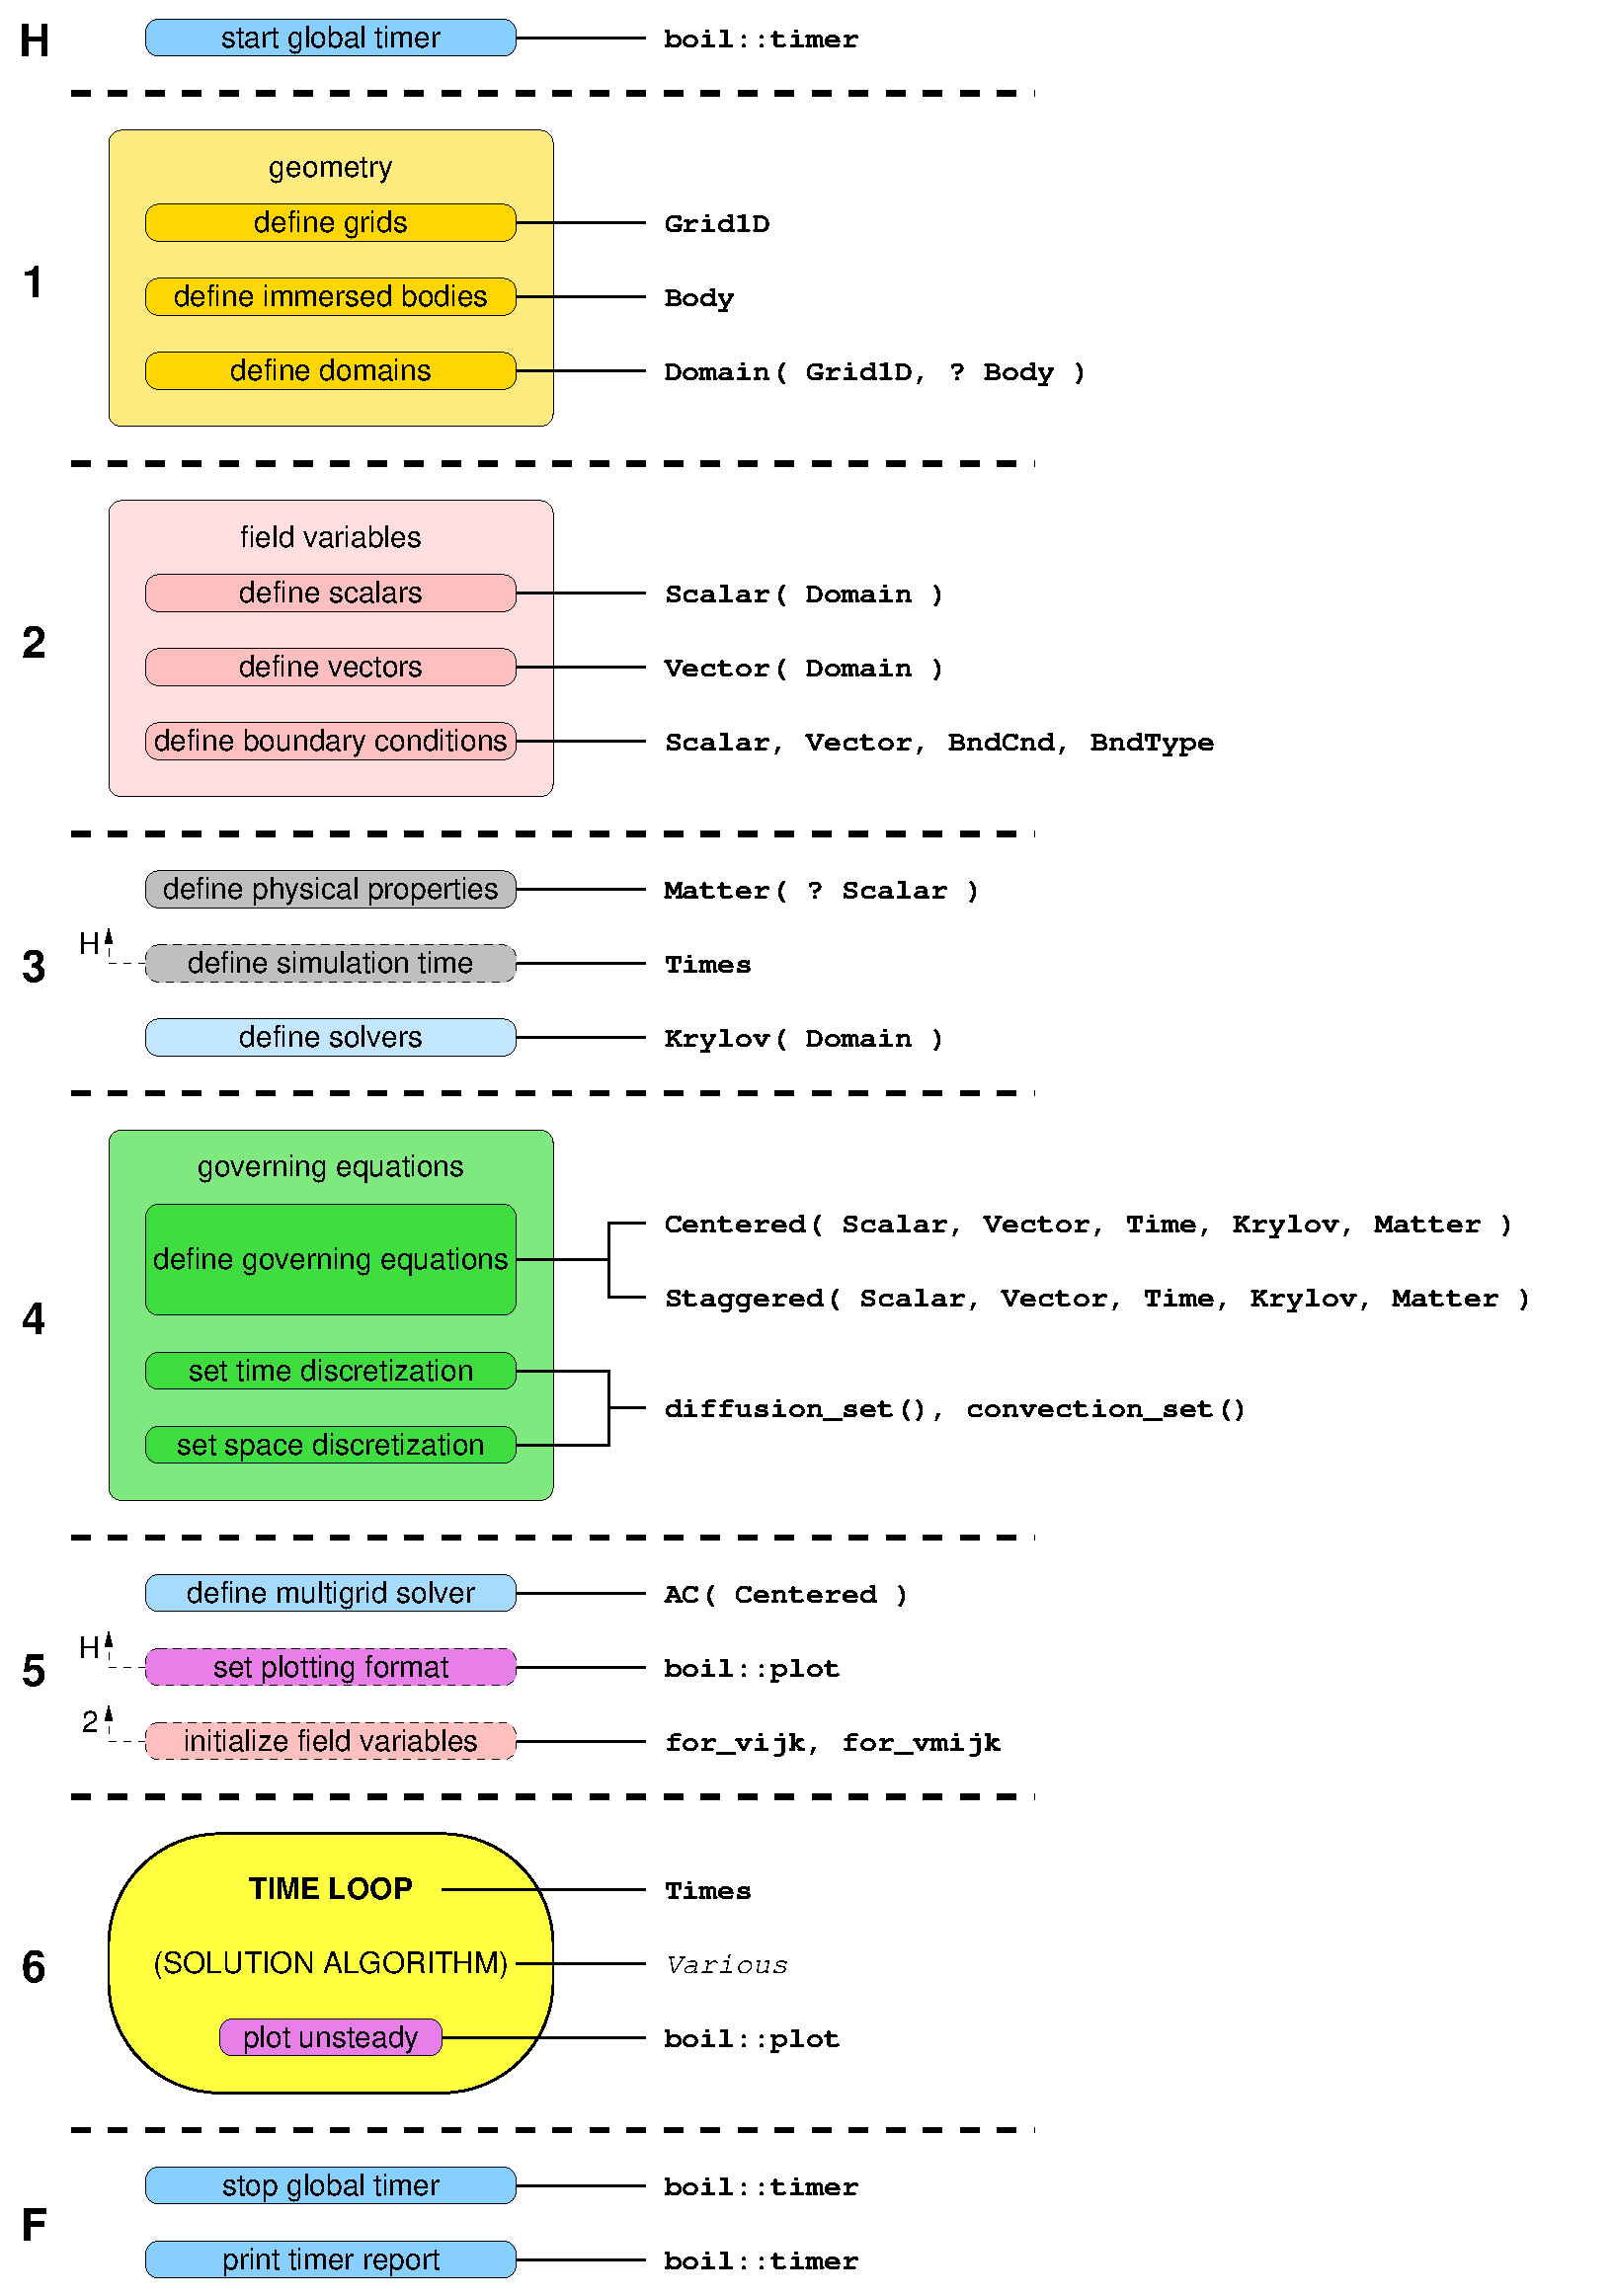
\includegraphics[scale=0.5]{Figures/08-01-structure.eps}}
  \end{picture}
  \caption{General structure of a {\psiboil} program.}
  \label{fig_structure}
\end{figure}

Header~(H) starts global object {\tt boil::timer}, while footer~(F)
stops it and prints the information on the CPU time on the terminal.
Header and footer must be present in every {\psiboil} program, because
many object use local timers to measure the performance of their
member functions. 

Quite naturally, right after the header, first unit starts which defines 
geometry (enclosed in an orange frame on~Fig.\ref{fig_structure}). 
Definition of geometry means defining grids ({\tt Grid1D}), IB's 
({\tt Body}) and domains ({\tt Domain}). 

Once the computational domain is defined, we can proceed with definition
of scalar and vector fields ({\tt Scalar} and {\tt Vector}) featured
in transport equations being solved. As soon as their are defined,
boundary conditions should be imposed on them as well. 

Third unit is a bit heterogeneous. It defines physical properties ({\tt Matter})
which depends on {\tt Scalar} in case of multiphase flows\footnote{That will
be covered in later chapters.}. Simulation time is also placed in this unit,
although it could have been defined right after the header. We prefer to put
it here for convenience, just to be closer to governing equations unit which
uses it as a parameter. Finally, solvers {\tt Krylov} are quite rigidly in
this unit. They must be defined after field variables and before governing
equations. 

Unit number four is dedicated to definition of governing equations. All the
equations are defined here (usually, that means: {\tt Momentum}, {\tt Pressure},
{\tt Enthalpy} \dots) as well as particular details about spatial and
temporal discretization. As far as spatial discretization is concerned,
various convection schemes can be defined (see the global class {\tt Limiter}
and associated ravioli class {\tt ConvScheme} in the directory: {\tt Src/Global}).
This feature is yet to be explored in the chapters below. Temporal discretization
schemes have been briefly touched upon in~Sec.~\ref{sub_sec_time_stepping}.

The following unit, number five, is actually a preparation for the time-loop.
As first, a multigrid solver ({\tt AC}) has to defined and it depends on the governing
equations. {\tt AC} is almost invariantly defined for pressure, while the other
variables, particularly when discretized for unsteady simulation, have 
well-conditioned linear systems and {\tt Krylov} solvers are usually efficient 
enough. Variables and source terms should be initialized before the time loop,
as well as plotting format. Both of these last two object could have been
defined much sooner. Variables could have been initialized right after their
definition, while the plotting format could have been chosen right after the
header (indicated with small arrows). 

Undoubtedly, the most important unit of the {\psiboil} is unit six,
the {\em Time loop}. It can be as simple as a single call to linear
solver\footnote{For example, line~38 in {\tt 07-01-main.cpp} is a complete
{\em Time loop}.} or as complex as time loop embedding another 
iterative procedure to couple various equations. This unit will vary
the most between different programs and different classes of problems
in particular. Therefore, it is beyond the scope of this chapter to
explain it any further. 

General structure of a {\psiboil} program, resembles two things: an
{\em input file} for a CFD package defining the problem to be solved 
(defining geometry, boundary conditions, material properties, choosing
plotting format, \dots), but also a flow diagram of a CFD program. 
In essence, it serves as both. As stated in Sec.~\ref{sec_about},
each problem solved with {\psiboil} requires a separate main program
(stored in {\tt main.cpp}), which used {\psiboil}'s objects to solve
a particular program. Each program defines geometry, boundary condition,
physical properties (units 1-4 in Fig.~\ref{fig_structure}), typical for 
an input file, but also defines the algorithm (units 5 and 6 
in Fig.~\ref{fig_structure}), as the flow diagram does. 
%
% really? When explaining the programs in the following chapters, we will try to
% really? explain them in parts corresponding to units introduced in this chapter. 

%---------------------------------------------------------------------nutshell-%
\vspace*{5mm} \fbox{ \begin{minipage}[c] {0.97\textwidth} %-----------nutshell-%
    {\sf Chapter \ref{chap_structure} in a nutshell} \\  %------------nutshell-%
   
      - Although {\psiboil} should be regarded as a collection of objects which
      facilitates the building of programs for numerical analysis of transport
      phenomena, each such program has a typical structure, represented
      in this chapter in form of a diagram. \\

      - The typical structure has six distinct units, in addition to header
      and footer. \\

      - This structure is flexible to some extent, but dependencies between
      the units introduce a certain order in which {\psiboil} objects are 
      laid out. \\

      - {\psiboil}'s main program (the one which is different for each problem
      solved) can be regarded as an input file for simulation and a flow
      diagram of the applied algorithm.

  \end{minipage} } %--------------------------------------------------nutshell-%
%---------------------------------------------------------------------nutshell-%
  

  %----------------------%
  %                      %
  %  Single-phase Flows  %
  %                      %
  %----------------------%
  \chapter{Single-phase Flows} 
  \label{chap_single_phase}

This chapter deals with the solution of transport equation for incompressible
fluid flow. The equation which describes this phenomenon is momentum
conservation equation, given by~\ref{eq_momentum}, repeated here for
convenience:
%
\be
         \int_V \frac{\p \rho \uvw}{\p t} dV
       + \int_S \rho \uvw \uvw \, dS
       = \int_S \mu \nabla \uvw \, dS
       - \int_V \nabla p \, dV
       + {\bf F}
       \; \; \; \;
       [N]
  \label{eq_momentum_2}
\ee
%
This form, however,
poses a problem. We have one three equations (one for each velocity 
component), but for unknowns: velocity components and pressure. 

For incompressible flow problems, pressure has always been sought through
additional constraint, mass conservation equation:
%
\be
       \int_V \frac{\p \rho}{\p t} dV 
       = 
       - \int_S \rho \uvw d{\bf S}
       \; \; \; \;
       [\frac{kg}{s}]
  \label{eq_mass}
\ee
% 
Momentum and mass conservation have been linked in various ways, providing
different algorithms for computation of incompressible flows. The most
widely used in applied CFD are SIMPLE, SIMPLEC, SIMPLER and even PISO 
({\bf references}). For highly unsteady flow, at simulation of which
{\psiboil} aims, the most efficient is the {\em fractional step method},
sometimes referred to as the {\em projection} method. It combines momentum
conservation equation~(\ref{eq_momentum}) with mass conservation
equation~(\ref{eq_mass}), at intermediate time between two simulated
time steps, to give additional equation for pressure (already introduced
as~\ref{eq_pressure}):
%
\be
         \int_S \frac{\nabla p}{\rho} \, d{\bf S} 
       = \frac{1}{\Delta t} \int_S \uvw^\s \, d{\bf S}
       \; \; \; \; 
       [ \frac{m^3}{s^2} ],
  \label{eq_pressure_2}
\ee
%
often referred to as pressure-Poisson equation.

The fractional step method, which is used by {\psiboil}, is now outlined.
The momentum conservation equation~(\ref{eq_momentum_2}) must first be discretized
in time, part by part. The most usual approach is to use Crank-Nicolson
scheme for diffusion (to avoid very low time steps needed by the forward
Euler scheme) and to use Adams-Bashforth for convection, for the sake
of simplicity. Inertial terms are discretized with backward Euler scheme.
The time-discretized momentum equation then looks like:
%
\be
        {\bf I}^\s - {\bf I}^{n-1} 
       + \frac{3}{2} {\bf C}^{n-1} - \frac{1}{2} {\bf C}^{n-2}
       = \frac{1}{2} {\bf D}^\s + \frac{1}{2} {\bf D}^{n-1}
       + {\bf F}^{n-1}
  \label{eq_semi}
\ee
%
Here, $\s$ denotes the tentative (intermediate) time step, while 
${\bf I}^\s = \frac{1}{\Delta t} \int_V  \rho \uvw^\s dV$ 
and ${\bf D}^\s = \int_S \mu \nabla \uvw^\s \, d{\bf S}$ 
denote inertial and diffusive term in the tentative time step. 
Old (known) values of velocity (at time step $n-1$) define terms:
${\bf I}^{n-1} = \frac{1}{\Delta t} \int_V  \rho \uvw^{n-1} dV$,
and ${\bf D}^{n-1} = \int_S \mu \nabla \uvw^{n-1} \, d{\bf S}$, as well
as convective term at old time step: 
${\bf C}^{n-1} = \int_S \rho \uvw^{n-1}\uvw^{n-1} \, d{\bf S}$. Clearly,
${\bf C}^{n-2} = \int_S \rho \uvw^{n-2}\uvw^{n-2} \, d{\bf S}$.

Equation~\ref{eq_semi} is discretized in space giving a linear system
of equations for intermediate velocity~($\uvw^\s$). Once this
system is solved gives velocity field which does not, generally, 
satisfies mass conservation equation. It is used to compute pressure 
from~\ref{eq_pressure_2}. The computed pressure is used to {\em project}
velocity into a divergence free velocity field:
%
\be
  \uvw^{n} = \uvw^\s + \frac{1}{\rho} \nabla p \, \Delta t
  \label{eq_projection}
\ee
%
which represents velocity at new time step. 

% wrong: {\psiboil} uses only fractional step method to link velocity and pressure.
% wrong: This also means that {\psiboil} can be used to simulate only unsteady 
% wrong: phenomena. If steady solution is sought, the governing equations should
% wrong: be integrated long enough until steady state is reached.


  \section{Flow over a cylinder}
\label{sec_cylinder}  

In this section, a flow over a cylinder is solved with {\psiboil}.
The flow is two-dimensional and isothermal and occurs at relatively low
Reynold number ($Re$). This problem will tech you how to define boundary
conditions for some parts of the boundary and is also a first fluid flow 
solver in this tutorial.

The geometry and boundary conditions are shown in~Fig.~\ref{fig_cylinder},
and dimensions are specified as following: $L=2.2$, $H=0.41$, and $W=H/2$.
Cylinder diameter is set to~$D=0.1$. Distance of cylinder axis to lower
corner of the inlet is~$h=0.2$, meaning the cylinder is not placed 
symmetrically in the problem domain. It is intentionally so, to promote
earlier transition to a vortex shedding regime. 

%------------%
%            %
%  Cylinder  %
%            %
%------------%
\begin{figure}[ht]
  \centering
  \setlength{\unitlength}{1mm}
  \begin{picture}(100, 43)(0,0)
    \thickbox{100}{ 43}
    \put(0,0){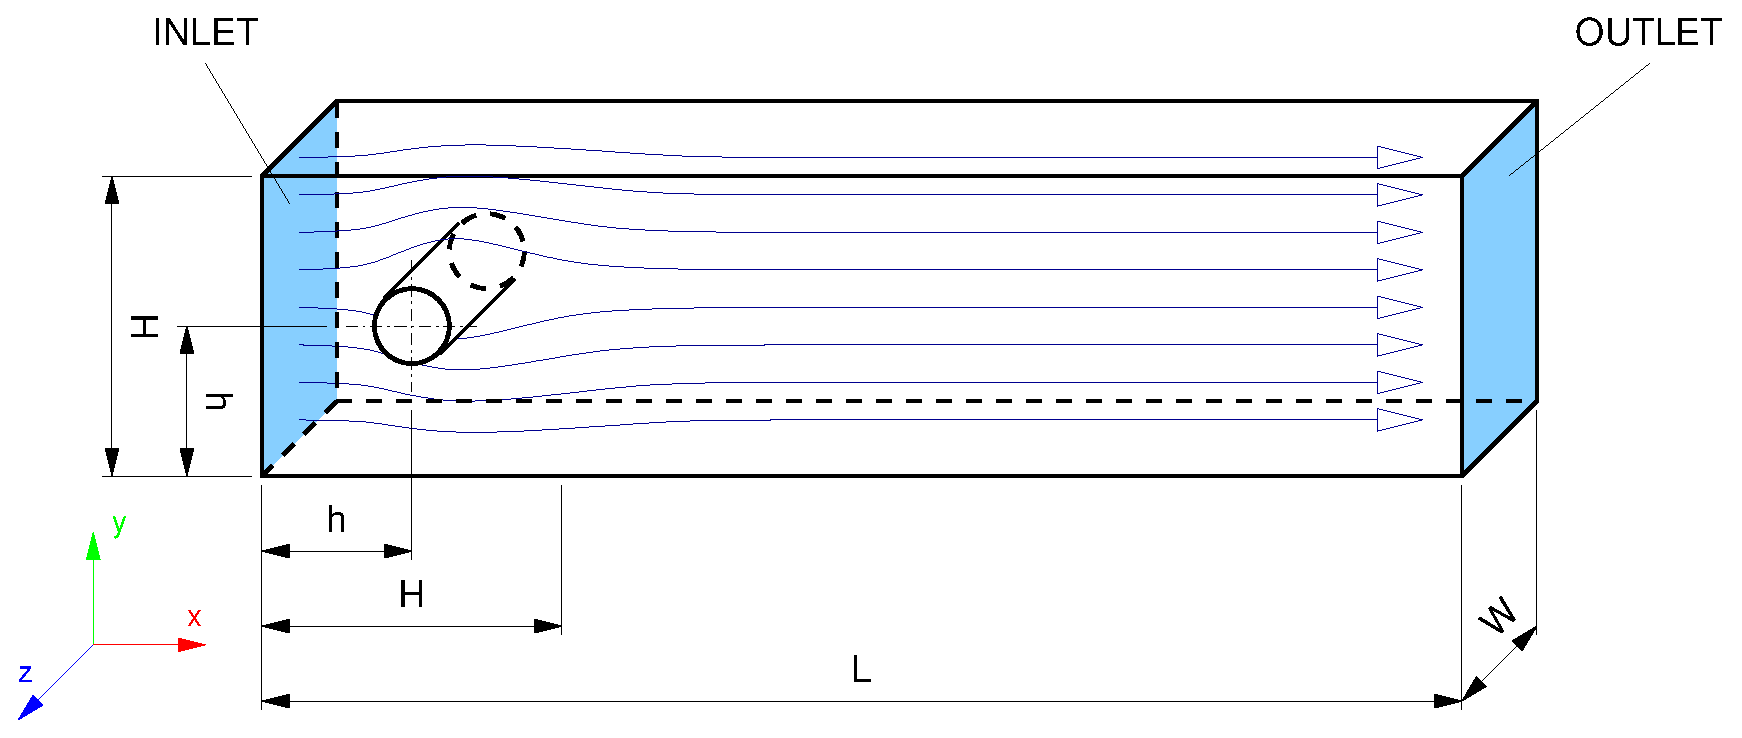
\includegraphics[scale=0.35]{Figures/09-01-domain.eps}}
  \end{picture}
  \caption{Geometry, boundary conditions and basic topology for the
           flow over a cylinder.}
  \label{fig_cylinder}
\end{figure}

Parabolic velocity profile is specified at the inlet according to the equation:
%
\be
  u = 4 \cdot U_m \cdot y \cdot (H-y)/H^2
\ee
%
where~$U_m$ is maximum inlet velocity equal to~1.5.

The program which solves this problem is stored under name {\tt 09-01-main.cpp}
and will be outlined in the rest of this chapter. However, different program
units, as outlined in Ch.~\ref{chap_structure}, will be introduced in separate
sub-sections. For the sake of shortness, some program comments will be skipped. 

Domain dimensions, as well as resolutions, are defined as constants outside
the body of the main function as:
%
{\small \begin{verbatim}
      3 /* dimensions */
      4 const real H  = 0.41;
      5 const real L  = 2.2;
      6
      7 /* resolutions */
      8 const int NY =  64;
      9 const int NX1 = NY;
     10 const int NX2 = NY;
     11 const int NZ  = NY/8;
\end{verbatim}}
%
The grid will be uniform in $y$ and $z$ (normal and span-wise), but
not in $x$ (stream-wise) direction. That is why we introduce two variables
for resolution in $x$, namely {\tt NX1} and {\tt NX2}.

\subsection{Domain}

IB, in this case cylinder, is defined in line 23:
%
{\small \begin{verbatim}
     23   Body cyl("09-01-cylinder.stl");
\end{verbatim}}
%
Clearly, cylinder is defined in STL format in file {\tt 09-01-cylinder.stl}, 
which must be present in the running directory. 

Grids are defined with the following lines:
%
{\small \begin{verbatim}
     28   Grid1D gz ( Range<real>(-H/4, H/4), NZ,  Periodic::yes());
     29   Grid1D gy ( Range<real>( 0.0, H  ), NY,  Periodic::no());
     30   Grid1D gx1( Range<real>( 0.0, H  ), NX1, Periodic::no());
     31   const real dx = H/(real)NY;
     32   Grid1D gx2( Range<real>( H,   L  ), Range<real>(dx, 8.0*dx), NX2, Periodic::no());
     33   Grid1D gx( gx1, gx2, Periodic::no());
\end{verbatim}}
%
No stretching is used in normal and span-wise ($y$ and $z$) direction. 
Span-wise direction is defined to be periodic. Grid in stream-wise~($x$)
direction is created from two parts: a {\em uniform} part, spanning 
from~$x=0$ to~$x=H$, created in line~30 as {\tt gx1} and a {\em non-uniform} 
one, spanning from~$x=H$ to~$x=L$, created in line~32 as~{\tt gx2}. 
The size of first cell in {\tt gx2} is set to be {\tt dx}, which corresponds
to cell size in~{\tt gx1}. Final grid in~$x$ direction is created in line~33
as a union of~{\tt gx1} and~{gx2}.

Once the IB and grids are defined, domain is created in line~38
with:
%
{\small \begin{verbatim}
     38   Domain d(gx, gy, gz, &cyl);
\end{verbatim}}

%--------%
%        %
%  Mesh  %
%        %
%--------%
\begin{figure}[h!]
  \centering
  \setlength{\unitlength}{1mm}
  \begin{picture}(140, 32)(0,0)
    \thickbox{140}{ 32}
    \put(0,-45){\includegraphics[scale=0.60]{Figures/09-01-mesh.eps}}
  \end{picture}
  \caption{Computational grid for the flow around a cylinder.}
  \label{fig_cylinder_mesh}
\end{figure}

\subsection{Field variables}

Now we have reached the second logical unit of the program, which defines
field variables. For this case, we have velocity and momentum forces
as {\tt Vector}'s and pressure and it's source as {\tt Scalars}, defined
in lines~40 and~41:
%
{\small \begin{verbatim}
     43   Vector uvw(d), xyz(d); /* velocity and its source */
     44   Scalar p  (d), f  (d); /* pressure and its source */
\end{verbatim}}
%
This is followed by the definition of boundary conditions. Since {\tt Vector}s
have three components, boundary conditions have to be assigned through a loop
browsing through them, as it is done in lines~49--57:
%
{\small \begin{verbatim}
     49   for_m(m) {
     50     uvw.bc(m).add( BndCnd( Dir::imin(), BndType::inlet(),
     51                    "4.0*1.5*y*(0.41-y)/0.41^2", "0.0", "0.0") );
     52     uvw.bc(m).add( BndCnd( Dir::imax(), BndType::outlet() ) );
     53     uvw.bc(m).add( BndCnd( Dir::jmin(), BndType::wall() ) );
     54     uvw.bc(m).add( BndCnd( Dir::jmax(), BndType::wall() ) );
     55     uvw.bc(m).add( BndCnd( Dir::kmin(), BndType::periodic() ) );
     56     uvw.bc(m).add( BndCnd( Dir::kmax(), BndType::periodic() ) );
     57   }
\end{verbatim}}
%
Browsing is performed with macro {\tt for\_m}, defined in {\tt Field/Vector/vector\_browsing.h}.
Variable representing vector component is defined as {\tt m} throughout {\psiboil}. It is a
ravioli object of type~{\tt Comp}.
Member function for defining boundary conditions for {\tt Vector}s defined from the one for
scalars (introduced in~Sec.~\ref{sub_sec_bc}) because it also has to provide the component for
which this boundary condition applies, i.e.\ the syntax of the member function is:
%
{\small \begin{verbatim}
     Vector::bc(Comp m).add( BndCnd & );
\end{verbatim}}
%
In lines~50--51 inlet is defined ({\tt BndType::inlet()}) at inlet plane ({\tt Dir::imin()}).
For velocity inlet, three values must be specified, one for each component. They are
defined in line~55 as: {\tt "4.0*1.5*y*(0.41-y)/0.41\^2"}, {\tt "0.0"} and {\tt "0.0"}.
{\psiboil} supports analytically prescribed boundary conditions, as long they are
functions of $x$, $y$ and $z$. For velocity outlet, as well as for wall and periodic
conditions, no values need to be specified, as shown in lines~52--56.

Boundary conditions for the pressure, when solved with the projection method, should
be $\frac{\p p}{\p n} = 0$ on all boundaries where velocities are known.
In this case, this are all, except the ones at periodic ones. All boundary conditions
for pressure are defined in lines~62--67:
%
{\small \begin{verbatim}
     59   p.bc().add( BndCnd( Dir::imin(), BndType::neumann() ) );
     60   p.bc().add( BndCnd( Dir::imax(), BndType::neumann() ) );
     61   p.bc().add( BndCnd( Dir::jmin(), BndType::neumann() ) );
     62   p.bc().add( BndCnd( Dir::jmax(), BndType::neumann() ) );
     63   p.bc().add( BndCnd( Dir::kmin(), BndType::periodic() ) );
     64   p.bc().add( BndCnd( Dir::kmax(), BndType::periodic() ) );
\end{verbatim}}
%
Note that boundary conditions have been defined for both variables at all 
boundary planes. No patch remained undefined. That is a {\em rule}. 
{\psiboil} {\em does not} support {\em default} boundary conditions for 
any variable. 

\subsection{Physical properties, time and solver}

We have reached the third unit (according to standard {\psiboil} program
layout outlined in~Fig.~\ref{fig_structure}, which defines physical 
properties ({\tt Matter}), simulation time ({\tt Times}) and linear
solver ({\tt Krylov}). In this program, the third unit looks like:
%
{\small \begin{verbatim}
     69   Matter fluid(d);
     70
     71   fluid.mu(0.001);
     72
     73   Times time(10000, dx/8.0);
     74
     75   Krylov * solver = new CG(d, Prec::di());
\end{verbatim}}
%
New substance is created with the name {\tt fluid} in line~69, and its
dynamic viscosity has been set to $0.001$ in line~71. Simulation time
is represented with object {\tt time}, created with number of time
steps equal to~10000 and time step equal to $\Delta t=dx/8$
The value of time step is calculated from the requirement 
that Courant-Friedrich-Levy (CFL) number is around $\frac{1}{4}$ during the
simulation\footnote{Keep in mind that maximum value of inlet velocity is~1.5
and that $\Delta x = dx$}. Time variable may be defined in
other ways. Instead of number of time steps and the time step value,
we could have defined total simulation time and number of time steps.
The details of these, and other possible definitions, take a look at
{\tt Src/Ravioli/times.h}.

\subsection{Transport equations}

Two transport equations are defined in the fourth unit, one for momentum
transport~(\ref{eq_momentum_2}) and one for pressure-Poisson~(\ref{eq_pressure_2}):
%
{\small \begin{verbatim}
     80   Pressure pr(p, f, uvw, time, solver, &fluid);
     81   Momentum ns( uvw, xyz, time, solver, &fluid);
\end{verbatim}}
%
Attributes sent to {\tt Pressure} constructor are the pressure {\tt p}
and its source {\tt f}, used for storing the right hand side 
of~Eq.~\ref{eq_pressure_2}, which is computed from velocity~{\tt uvw},
sent as a third parameter. {\tt Momentum} constructor takes velocity
field {\tt uvw} and its forces {\tt xyz} as parameters. Both 
{\tt Pressure} and {\tt Momentum} constructor need variable defining
simulation time, solver and substance, represented in lines~80
and~81 as objects {\tt time}, {\tt solver} and {\tt fluid}.

\subsection{Preparation for the time-loop}

The fifth unit contains only one line:
%
{\small \begin{verbatim}
     83   AC multigrid( &pr );
\end{verbatim}}
%
which creates a multigrid solver for the {\tt Pressure p}. When solving
transient transport equations, it is sound to create a multigrid solver
for pressure only. Transported variables (momentum, enthalpy, \dots)
give well-conditioned systems which can be solved with {\tt Krylov}
solver only. Even more, multigrid solver {\em can not} be defined
for momentum equations, since they change their resolution due to
staggered arrangement of variables. No variable needs initialization for 
this problem.

This program features modest $Re$, but for this geometry, it should yield
and oscillatory solution, {\em i.e.} it should lead to  vortex shedding.
Therefore, it would be convenient if {\psiboil} was printing the value 
of certain variable at a point in the domain during the simulation to check
whether an oscillatory solution has been reached, or to check the frequency
of oscillations, etc. There is a class which does just that. It is 
called~{\tt Location} and is defined in {\tt Src/Monitor/Location}.
Here, we define a {\tt Location} as:
%
{\small \begin{verbatim}
     85   Location loc("monitor", d, NX1, NY/2, NZ/2);
\end{verbatim}}
%
It creates {\tt Location loc}, called {\tt "monitor"}, in the {\tt Domain d},
at logical coordinates ($i$, $j$ and $k$) equal to {\tt NX1}, {\tt NY/2}, 
and {\tt NZ/2}. That {\tt Location} will be placed midway between the walls
in the region where uniform~({\tt gx1}) and non-uniform~({\tt gx2}) grids
meet. It's usage is explained below. 

\subsection{The time-loop}

Finally, we reach the time loop of the program, reading:
%
{\small \begin{verbatim}
     90   for(time.start(); time.end(); time.increase()) {
     91
     92     boil::oout << "##################" << boil::endl;
     93     boil::oout << "#                 " << boil::endl;
     94     boil::oout << "# TIME:      " << time.current_time() << boil::endl;
     95     boil::oout << "#                 " << boil::endl;
     96     boil::oout << "# TIME STEP: " << time.current_step() << boil::endl;
     97     boil::oout << "#                 " << boil::endl;
     98     boil::oout << "##################" << boil::endl;
     99
    100     ns.cfl_max();
    101
    102     ns.new_time_step();
    103
    104     ns.solve(ResRat(1e-2));
    105
    106     p = 0.0;
    107
    108     multigrid.vcycle(ResRat(1e-2));
    109
    110     ns.project(p);
    111
    112     loc.print(uvw, Comp::v());
    113
    114     if( time.current_step() % 100 == 0)
    115       boil::plot->plot(uvw,  p, "uvw,p",  time.current_step());
    116   }
\end{verbatim}}
%
This loop embodies an implementation of fractional step algorithm in {\psiboil}.
In line~90 you can see how can variable {\tt time} be used to cycle through time.
It's member functions {\tt Times::start()}, {\tt Times::end()} and {\tt Times::increase()}
serve as parts of {\tt C++}'s {\tt for} loop. The advantage is that this loop 
remains the same, no matter how the variable {\tt time} was defined. 
Two additional {\tt Times}' member functions are used to plot current simulation
time and time step in lines~94 and~96. 

Line~100 calls {\tt Momentum}'s member function {\tt Momentum::cfl\_max} which computes
and prints the value of CFL number. Is it not necessary to call it, but it may serve
as a good indication why a certain simulation crashed\footnote{If CFL numbers gradually
increase, and gradually reach values higher than 0.5, simulation will be inaccurate
and will probably crash due to a too high time step.}. If CFL is too low, on the
other hand, we are wasting a lot of computational time. As a {\em rule of thumb}, optimum
CFL is in the range from $0.35 - 0.4$. 

Preparation for the new time step (which involves computation of terms with 
superscript~$n-1$ and~$n-2$ in Eq.~\ref{eq_semi}) are performed at line~102. That
is followed by it's solution at line~104. At that point, we have tentative 
velocity ($\uvw^\s$). 

In line~108, {\psiboil} uses the tentative velocity field to compute the right hand
side of~Eq.\ref{eq_pressure_2} and solve it to get the new pressure field. For unsteady
simulations, convergence of the multigrid solution for the pressure usually improves
if pressure is initialized to zero. It is performed in line~106. 

This pressure field is used to {\em project} tentative velocity ($\uvw^\s$)
into a new ($n$) divergence-free field~($\uvw^n$). This closes the fractional
step algorithm for one time step, and the new one can start. 

Line~112 shows how can an object of type {\tt Location} be conveniently used to
monitor the computed values. It prints the value of the argument (here {\tt Vector}
and it's component) at position defined in line~91, during the construction of
{\tt Location}. 

The programs plots the results (for velocities and pressure) every~100$^{th}$ from
lines~114 and~115.

\subsection{Running the program}  

Compile and run this program. Run it with:
%
\begin{verbatim}
> ./Boil > out &
\end{verbatim}
%
to store the terminal output to file {\tt "out"}. This simulation might take few hours
to finish. If you would like to check the progress during the run, issue the
command:
%
\begin{verbatim}
> tail -100f out
\end{verbatim}
%
As an example, output for time step~20 looks like:
%
{\small \begin{verbatim}
##################
#
# TIME:      0.0152148
#
# TIME STEP: 20
#
##################
cfl max = 0.230888 in direction u  at: 0.192187 0.265859 -0.0384375
u, residual = 6.87374e-07, ratio = 0.000281587
v, residual = 4.13061e-07, ratio = 0.000270693
w, residual = 2.03872e-08, ratio = 0.000250742
FILE: momentum_scale_out.cpp, LINE: 24, volf_in = 0.0840603
FILE: momentum_scale_out.cpp, LINE: 77, ratio = 1.00061
@get_src; err sou = 0.471205 -0.0399352
Initial  res = 0.00387017
Cycle 1; res = 0.000186533
Cycle 2; res = 8.59826e-05
Cycle 3; res = 2.87255e-05
Converged in 3 cycles!
monitor: -0.00159419
\end{verbatim}}
%
The lines beginning with a {\tt \#} only mark the beginning of a time step.
CFL is printed right after that. The following two lines show the result
of solving of momentum equations. {\tt residual} is the residual of 
the solving procedure, and {\tt ratio} shows the level of reduction of
residuals in the solvers. (For example, for {\tt w}, residuals were
reduced by roughly $4000$ times).
%
The following two lines (beginning with {\tt FILE}), are actually the
development lines (see Sec.~\ref{sec_development}) which print the inlet bulk
velocity and the ratio between inlet and outlet bulk velocities. The former
depends on inlet boundary condition, while the latter should always be
close to unity. 
%
Line beginning with {\tt @get\_src} prints the square and absolute integral
of mass error created by tentative velocity field. While the square of the
error may have any value, absolute integral should be as close to zero as
possible. 

The line which follows shows the residual history of the multigrid algorithm.
The final line is the output created by program line~112, i.e.\ by {\tt Location}.
It can be used to plot the history of $v$ velocity component. 
%
Here is 
a simple way how to do it. Once the simulation is finished, run the 
command:
%
\begin{verbatim}
> cat out | grep monitor > monitor.dat
\end{verbatim}
%
That will create the file {\tt "monitor.dat"} which looks like:
%
{\small \begin{verbatim}
      1 Location monitor at x = 0.406797, y = 0.201797, z = -0.0128125 created.
      2 monitor: -0.00246605
      3 monitor: -0.002181
      4 monitor: -0.00406565
      5 monitor: -0.00401776
      6 monitor: -0.00400525
      7 monitor: -0.00399137
      8 monitor: -0.00392429
      ...
\end{verbatim}}
%
Erase the first line, and all occurrences of: {\tt "monitor:"} to get a file like:
%
{\small \begin{verbatim}
      1  -0.00246605
      2  -0.002181
      3  -0.00406565
      4  -0.00401776
      5  -0.00400525
      6  -0.00399137
      7  -0.00392429
      ...
\end{verbatim}}
% 
You could have also created such a file using three UNIX commands {\tt cat},
{\tt grep} and {\tt awk} in a single line:
%
\begin{verbatim}
cat out | grep monitor | awk '{print $2}' > monitor.dat
\end{verbatim}
%
Plot this line using {\tt grace} or {\tt gnuplot} to see the time-history. It
is plotted in Fig.~\ref{fig_monitor}. You can clearly see the history of $v$ velocity
component at $x=0.41$, $y=0.2$ and $z=0.0$. Obviously the flow has reached oscillatory
regime.

%------------------%
%                  %
%  u time history  %
%                  %
%------------------%
\begin{figure}[ht]
  \centering
  \setlength{\unitlength}{1mm}
  \begin{picture}( 75, 52)(0,0)
    \thickbox{ 75}{ 52}
    \put(0,0){\includegraphics[scale=0.3]{Figures/09-01-monitor.eps}}
  \end{picture}
  \caption{Time-history of $u$ velocity component at $x=0.41$, $y=0.2$ and $z=0.0$.}
  \label{fig_monitor}
\end{figure}

\subsection{Results and footer output}  

Just before the end of the time loop, there are lines for creating results: 
%
{\small \begin{verbatim}
    114     if( time.current_step() % 100 == 0)
    115       boil::plot->plot(uvw,  p, "uvw,p",  time.current_step());
\end{verbatim}}
%
These lines save results for velocity and pressure every 100 time steps in files called:
{\tt uvw,p\_p000\_0100.dat}, {\tt uvw,p\_p000\_0200.dat}, {\tt uvw,p\_p000\_0300.dat}, etc.
Visualization of pressure and velocity field for the final time step is given 
in~Fig.~\ref{fig_cylinder_results_pressure} and Fig.~\ref{fig_cylinder_results_velocity}
respectivelly..

%------------------%
%                  %
%  Pressure field  %
%                  %
%------------------%
\begin{figure}[ht]
  \centering
  \setlength{\unitlength}{1mm}
  \begin{picture}(140, 33)(0,0)
    \thickbox{140}{ 33}
    \put(0,-45){\includegraphics[scale=0.60]{Figures/09-01-pressure.eps}}
  \end{picture}
  \caption{Pressure field at the end of simulation.}
  \label{fig_cylinder_results_pressure}
\end{figure}

%------------------%
%                  %
%  Velocity field  %
%                  %
%------------------%
\begin{figure}[ht]
  \centering
  \setlength{\unitlength}{1mm}
  \begin{picture}(140, 33)(0,0)
    \thickbox{140}{ 33}
    \put(0,-45){\includegraphics[scale=0.60]{Figures/09-01-streamlines.eps}}
  \end{picture}
  \caption{Stream-lines colored with stream-wise velocity component at the 
           end of simulation.}
  \label{fig_cylinder_results_velocity}
\end{figure}

At the end of simulation, you will get the following information in the file
{\tt out}, to which the terminal output is redirected:
%
{\small \begin{verbatim}
+==========================================
| Total execution time: 7857.54 [s]
+------------------------------------------
| Time spent in bounding box       : 0.01 [s]    (0.00127267%)
| Time spent in cell cutting       : 0.04 [s]    (0.00509068%)
| Time spent in flood fill         : 0.05 [s]    (0.00636335%)
| Time spent in plotting           : 59.22 [s]    (0.75342%)
| Time spent in pressure discretize: 0.01 [s]    (0.00127267%)
| Time spent in momentum discretize: 0.07 [s]    (0.00890869%)
| Time spent in momentum solver    : 428.55 [s]    (5.45339%)
| Time spent in vcycle             : 5885.13 [s]    (74.8979%)
| Time spent in coarsening         : 6.9 [s]    (0.878142%)
| Time spent elsewhere             : 1413.92 [s]    (17.9943%)
+------------------------------------------
\end{verbatim}}
%
As stated above, quite a few {\psiboil} objects have built-in local
timers. Here you see a typical situation: pressure solution, since
the system is poorly conditioned, takes almost~$75 \%$ of CPU-time. 
Momentum equations, thanks to unsteady term which conditions the
system well, takes slightly more than~$5 \%$, a staggering difference.

%---------------------------------------------------------------------nutshell-%
\vspace*{5mm} \fbox{ \begin{minipage}[c] {0.97\textwidth} %-----------nutshell-%
    {\sf Section \ref{sec_cylinder} in a nutshell} \\  %--------------nutshell-%
   
      - When prescribing boundary condition for velocity, it must be done for
      {\em each} component. \\

      - {\psiboil} supports analytically prescribed values for boundary conditions
      as long as they are functions of coordinates $x$, $y$ and $z$. \\

      - Periodic boundary condition {\em must} be imposed on the variable, regardless
      of the fact periodicity has been defined for the grid. \\

      - Boundary conditions should be prescribed for {\em all} boundaries. \\

      - There is {\em no} default boundary condition in {\psiboil}. \\

      - {\tt Momentum}'s member function {\tt Momentum::cfl\_max} can be used 
      to check whether the time step is appropriate for the simulation. \\

      - If CFL exceeds the value of 0.5, the simulation will likely become 
      unstable. \\

      - As a {\em rule of thumb}, it is good to chose a time step which gives
      CFL around 0.35. \\

      - Object of type {\tt Location} can be used to monitor time-histories
      of the solution at specified locations inside the computational {\tt Domain}.
 
  \end{minipage} } %--------------------------------------------------nutshell-%
%---------------------------------------------------------------------nutshell-%

  \section{Thermally-driven cavity flow}
\label{sec_thermally}  

This case was chosen to demonstrate the coupling of enthalpy and momentum equations.
The problem is illustrated in~Fig.~\ref{fig_thermally}. It is a cavity with a
square-shaped cross-section, with differentially heated side walls. Top and
bottom walls are insulated. Buoyancy forces give rise to circular motion of
the fluid inside the cavity. 

%---------------------------%
%                           %
%  Thermally-driven cavity  %
%                           %
%---------------------------%
\begin{figure}[ht]
  \centering
  \setlength{\unitlength}{1mm}
  \begin{picture}( 55, 53)(0,0)
    \thickbox{ 55}{ 53}
    \put(0,0){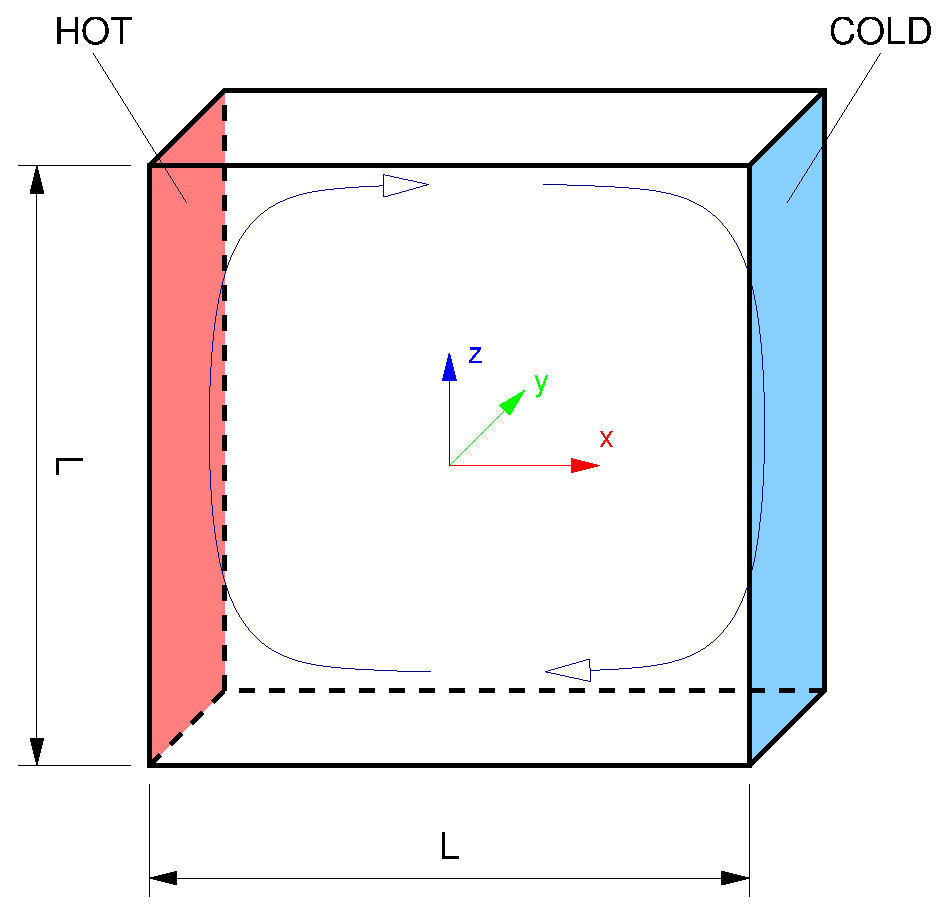
\includegraphics[scale=0.35]{Figures/09-02-thermally.eps}}
  \end{picture}
  \caption{Geometry, boundary conditions and basic topology for the 
           thermally-driven cavity flow.} 
  \label{fig_thermally}
\end{figure}

The program which solves this problem is stored as: {\tt 09-02-main.cpp}.
The features which are new for this problem are described in detail, while the
concepts which have already been explained above (grid generation, boundary
conditions, etc.) are merely mentioned. 

The governing equations in non-dimensional form read:
%
\be
         \int_{V^\s} \frac{\p T^\s}{\p t^\s} dV^\s
       + \int_{S^\s} \uvw^\s T^\s \, d{\bf S}^\s
       = \int_{S^\s} \nabla T^\s \, d{\bf S}^\s
   \label{eq_enthalpy_nd}
\ee
%
\be
         \int_{V^\s} \frac{\p \rho \uvw^\s}{\p t^\s} dV^\s
       + \int_{S^\s} \uvw^\s \uvw^\s \, dS^\s
       = Pr \int_{S^\s} \nabla \uvw \, dS^\s
       - \int_{V^\s} \nabla p^\s \, dV^\s
       + Ra Pr \int_{V^\s} {\bf d} \theta \, dV^\s
   \label{eq_momentum_nd}
\ee
%
if the scales for length, velocity, time and pressure are $L$, ${\alpha}/{L}$
${L^2}/{\alpha}$ and ${\alpha^2 \rho}/{L^2}$ respectively. 
Here~$\alpha = {\lambda}/({\rho C_p)}$ is thermal diffusivity coefficient.
Non-dimensional temperature is defined as 
$T^\s = (T - T_C)/(T_H-T_C)$
%
This problem can be fully characterized with two non-dimensional numbers:
the Rayleigh ($Ra = \rho g \beta \Delta T L^3 / \mu \alpha$) and the 
Prandtl ($Pr =  \alpha \rho / \mu$) number. 
These two numbers are defined as a constants at the beginning of the
program:
%
{\small \begin{verbatim}
     10 const real Pr = 0.71;
     11 const real Ra = 1.0e+5;
\end{verbatim}}
%
The problem is two-dimensional, but {\psiboil} can not handle purely two-dimensional
grids. Two-dimensionality can be {\em mimicked} by imposing the periodicity in the
homogeneous direction. This is achieved by the following part of the code:
%
{\small \begin{verbatim}
      4 const real LX =   1.0;
      5 const real LY =   0.125;
      6
      7 const int NX = 64;
      8 const int NY =  4;
     ...
     18   /*----------+
     19   |  grid(s)  |
     20   +----------*/
     21   Grid1D gx( Range<real>( -0.5*LX, 0.5*LX ), NX, Periodic::no());
     22   Grid1D gy( Range<real>( 0, LY ),           NY, Periodic::yes());
     ...
     27   Domain d(gx, gy, gx);
\end{verbatim}}
%
As defined in~Fig.~\ref{fig_thermally}, homogeneous direction is~$y$. The resolution
in $y$ direction is only four cells, a {\em minimum} resolution which can be defined
in {\psiboil}.

For this case, we need variables for temperature, enthalpy source, momentum and its
force, pressure and its source. They are defined with:
%
{\small \begin{verbatim}
     32   Vector uvw(d), xyz(d); // vel
     33   Scalar p  (d), f  (d); // p.
     34   Scalar t  (d), g  (d); // t.
\end{verbatim}}
%
Boundary conditions are defined in lines~39--60, and need no further explanation. 
It is maybe worth reminding that periodic boundary conditions must be set to
variables, notwithstanding they were defined for grids. 

Boundary condition section is followed by the definition of physical properties.
This is a particular case, solved in non-dimensional form 
(Eq.~\ref{eq_enthalpy_nd}~and~\ref{eq_momentum_nd}), so the
only "property" which has to be changed is "dynamic viscosity":
%
{\small \begin{verbatim}
     65   Matter fluid(d);
     66   fluid.mu( Pr );
\end{verbatim}}
%
Setting the number of time steps and selection of Krylov solver are done in 
lines~68 and ~70, and need no further explanation. 
Pressure-Poisson equation, as well as transport equations are defined in lines~75--77:
%
{\small \begin{verbatim}
     75   Pressure pr  ( p,   f,   uvw, time, solver, &fluid);
     76   Momentum ns  ( uvw, xyz,      time, solver, &fluid);
     77   Enthalpy enth( t,   g,   uvw, time, solver, &fluid);
\end{verbatim}}
%
Just before the time loop, multigrid solver is defined in line~79 and
a monitoring location (called {\tt m0}) in line~81:
%
{\small \begin{verbatim}
     79   AC multigrid( &pr );
     80
     81   Location m0("m0", d, NX/2, NY/2, NX/4);
\end{verbatim}}
%

Finally, we reach the time loop, which, in essence, is an {\em evolution} of
the one presented in~Sec.~\ref{sec_cylinder}:
%
{\small \begin{verbatim}
     83   for(time.start(); time.end(); time.increase()) {
     ...
     93     enth.new_time_step();
     94     enth.solve(ResRat(0.001));
     95
     96     ns.cfl_max();
     97     ns.new_time_step();
     98
     99     Comp m = Comp::w();
    100     for_vmijk(xyz,m,i,j,k)
    101       xyz[m][i][j][k] = Pr*Ra * 0.5*(t[i][j][k]+t[i][j][k-1]) * xyz.dV(m,i,j,k);
    102
    103     ns.solve(ResRat(0.001));
    104
    105     multigrid.vcycle(ResRat(0.001));
    106     
    107     ns.project(p);
    108
    109     pr.update_rhs();
    110
    111     m0.print(uvw,Comp::u());
    112   }
\end{verbatim}}
%
Each time step starts with computation of enthalpy. That is possible, because
convective terms are discretized with Adams-Bashforth time stepping scheme, 
meaning that it uses velocity and temperature field in old time step~($n-1$)
and the time step before old~($n-2$). Right-hand side of enthalpy equation
is assembled in line~93, and the linear solver is invoked from line~94.

That is followed by computation of momentum equations. Right hand side terms
depending on old time steps are computed in line~97. For this case, however,
that is not all. Temperature field is coupled with momentum equations
via the Boussinesq approximation defined in lines~99--101. It is worth noting
that macro {\tt for\_vmijk} has been used again, with parameter~{\tt m} specifying
the direction in which the buoyancy acts. It is worth noting
that even for this case, the right hand side is integrated over cell using mid-point
rule, i.e.: multiplying the source with cell volume. Cell volume is stored in
{\tt Vector}'s member function {\tt Vector::dV(m,i,j,k)} which, unlike the {\tt Scalar}'s
variant takes one parameter more, for vector component. The reason for that lies in
the fact that cells of a staggered generally have different volumes than centered cells,
as illustrated in~Fig.~\ref{fig_staggered_cell}.

%------------------%
%                  %
%  Staggered cell  %
%                  %
%------------------%
\begin{figure}[ht]
  \centering
  \setlength{\unitlength}{1mm}
  \begin{picture}( 65, 42)(0,0)
    \thickbox{ 65}{ 42}
    \put(0,0){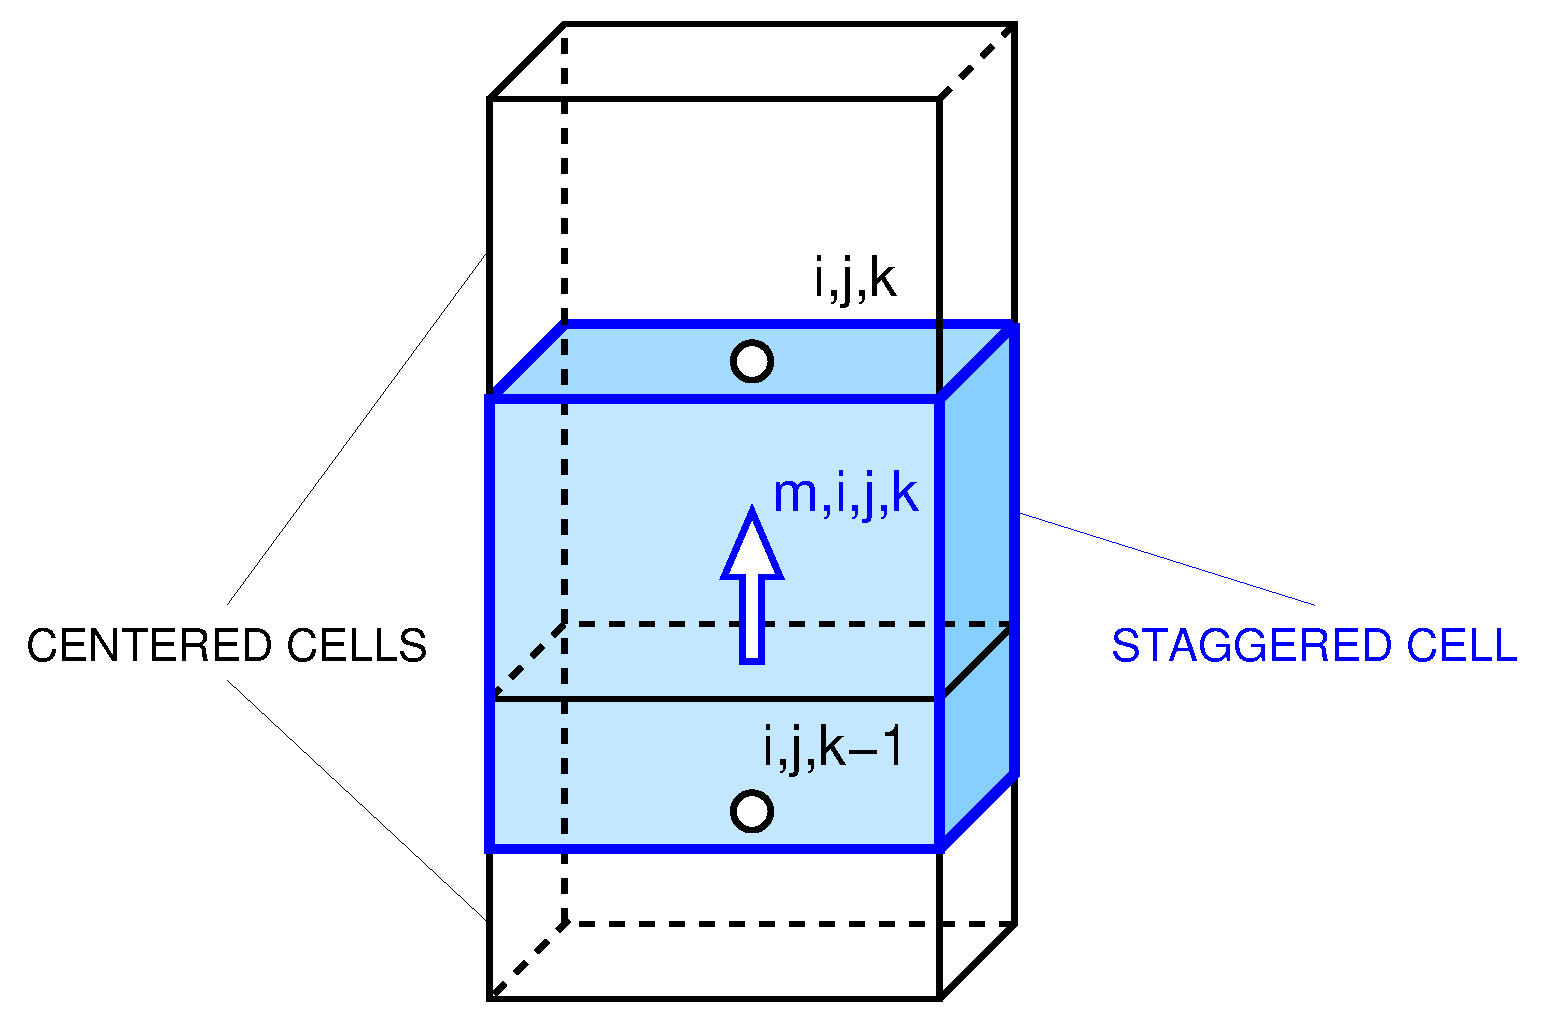
\includegraphics[scale=0.25]{Figures/09-02-staggered-cell.eps}}
  \end{picture}
  \caption{Volume of a staggered ({\tt Vector}'s) cell is different from volume of a 
           centered ({\tt Scalar}'s) cell.
           {\tt Scalar::dV(i,j,k)} $\neq$ {\tt Vector::dV(m,i,j,k)}}
  \label{fig_staggered_cell}
\end{figure}

Figure~\ref{fig_staggered_cell} also makes it clear why temperature for the source
term in program line~101 is taken as an arithmetic average between {\tt t[i][j][k]} 
and {\tt t[i][j][k-1]}.

Lines~103-107 are the same as in~Sec.~\ref{sec_cylinder} and need no explanation. 
A novelty is in line~109, which calls for an explicit update\footnote{It is called 
implicitly from {\tt multigrid.vcycle(ResRat(0.001));}.} of the right-hand side of 
pressure-Poisson equation. It is a trick to  get the mass (im)balance after the
projection of velocities into a divergence-free field. To illustrate it, it is
worth taking a look at the part of the output of this program:
%
{\small \begin{verbatim}
@get_src; err sou = 1.59193 4.2526e-12
Initial  res = 4.68899e-08
Cycle 1; res = 2.01202e-08
Cycle 2; res = 1.61724e-09
Cycle 3; res = 2.19523e-10
Cycle 4; res = 3.98007e-11
Converged after 4 cycles!
@get_src; err sou = 4.37667e-12 6.17362e-14
\end{verbatim}}
%
Compare two lines beginning with {\tt @get\_src}. Te first one is result of implicit
call from line~105, while the last is result of explicit call from line~109. 
Comparing the first number of the two ({\tt 1.59193} and {\tt 4.37667e-12}), 
gives an indication of the success of projection step. In this case, it is
very successful, since projection step reduces mass error by many orders of
magnitude. 

Program line~111 produces time history of $u$ velocity component, plotted 
in~Fig.~\ref{fig_monitor_2}. It is quite convincing that simulation has
reached the steady state. 

%------------------%
%                  %
%  u time history  %
%                  %
%------------------%
\begin{figure}[ht]
  \centering
  \setlength{\unitlength}{1mm}
  \begin{picture}( 75, 52)(0,0)
    \thickbox{ 75}{ 52}
    \put(0,0){\includegraphics[scale=0.3]{Figures/09-02-monitor.eps}}
  \end{picture}
  \caption{Time-history of $u$ velocity component at $x=-0.01$, $y=-0.05$ and $z=-0.26$.}
  \label{fig_monitor_2}
\end{figure}

\subsection{Results and footer output}  

Results, plotted from lines~114--116 (not shown here) are displayed in 
Fig.~\ref{fig_thermally_results}. 

%----------------------------------%
%                                  %
%  Temperature and velocity field  %
%                                  %
%----------------------------------%
\begin{figure}[ht]
  \centering
  \setlength{\unitlength}{1mm}
  \begin{picture}(140, 60)(0,0)
    \thickbox{140}{ 60}
    \put(70, 0){\includegraphics[scale=0.30]{Figures/09-02-velocity.eps}}
    \put( 0, 0){\includegraphics[scale=0.30]{Figures/09-02-temperature.eps}}
  \end{picture}
  \caption{Non-dimensional temperature (left) and velocity field (right) for 
           the thermally driven cavity at $Pr=0.71$ and $Ra=10^5$.}             
  \label{fig_thermally_results}
\end{figure}

Imagine you wanted to extract some profiles from the results, say~$u$~velocity
profile at~$x=0$ and~$w$~velocity profile at~$z=0$. These profiles might be
extracted from Tecplot, which was used to create plots in~Fig.~\ref{fig_thermally_results},
but that will not give the values computed by~{\psiboil}, but rather 
interpolations of these results performed internally by Tecplot. 

{\psiboil} offers a class which can extract profiles from solution, in much the 
same way certain locations in the computational {\tt Domain} are monitored with
the object of type {\tt Location}. The class which extract profiles is called
{\tt Rack}, defined in {\tt Src/Monitor/Rack}, and its usage is demonstrated in lines:
%
{\small \begin{verbatim}
    118   Rack    r0("u-comp", d, NX/2+1, NY/2, Range<int>(1,NX));
    119   Rack    r2("w-comp", d, Range<int>(1,NX), NY/2, NX/2+1);
    120   r0.print(uvw,Comp::u());
    121   r2.print(uvw,Comp::w());
\end{verbatim}}
%
Line~118 creates a measuring {\tt Rack} named {\tt "u-comp"} in {\tt Domain d},
at logical coordinates:~($i$ and~$j$) equal to~{\tt NX/2+1} and~{\tt NY/2} while
ranging in $k$ direction from {\tt 1} to~{\tt NX}. This {\tt Rack} extracts
$u$~velocity component in line~120. 
Line~119 creates a {\tt Rack} oriented in $i$~direction while line~121 extract 
$w$~velocity profile from it. These profiles are printed on 
terminal\footnote{or in a file to which the terminal output was redirected 
with {\tt ./Boil > out \&}} and this printing appears as:
%
{\small \begin{verbatim}
Rack:u-comp
0.0078125 0.046875 -0.492188 -3.7066
0.0078125 0.046875 -0.476562 -10.3498
0.0078125 0.046875 -0.460938 -16.309
0.0078125 0.046875 -0.445312 -21.5107
0.0078125 0.046875 -0.429688 -25.8977
...
\end{verbatim}}
%
which list~$x, y, z$ coordinates, followed by value of $u$~velocity component.
These lists should be extracted from and saved in a separate file. A plot
of these two profiles is shown in~Fig.~\ref{fig_thermally_profiles}.

%-----------------------------%
%                             %
%  u and w velocity profiles  %
%                             %
%-----------------------------%
\begin{figure}[ht]
  \centering
  \setlength{\unitlength}{1mm}
  \begin{picture}(140, 60)(0,0)
    \thickbox{140}{ 60}
    \put( 0, 0){\includegraphics[scale=0.35]{Figures/09-02-u.eps}}
    \put(70, 0){\includegraphics[scale=0.35]{Figures/09-02-w.eps}}
  \end{picture}
  \caption{Non-dimensional $u$~velocity distribution along the line~$x=0$ (left)
           and $w$~velocity distribution along the line~$z=0$.}
  \label{fig_thermally_profiles}
\end{figure}

The profiles in~Fig.~\ref{fig_thermally_profiles} give quantitative data, but
velocity components are not usually reported for this case. It is the Nusselt
number~($Nu = {\p T^\s}/{\p n^\s}$) which is the target 
benchmark datum.
%
As with velocity profiles, it is quite dangerous to extract this value from
post-processing tool, since it is based on internal approximations done in the
tool. The value of $Nu$ which is really computed in {\psiboil} {\em must} be
extracted from the program itself. For this case, it is done with the
following piece of coding:
%
{\small \begin{verbatim}
    123   const int ii = t.si();   /* i inside the domain */
    124   const int iw = ii-1;     /* i in the wall */
    125   const int j  = t.ej()/2; /* j in the middle */
    126   boil::oout << " Nusselt number " << boil::endl;
    127   for_vk(t,k) {
    128     real nu = (t[iw][j][k] - t[ii][j][k]) / t.dxw(ii);
    129     boil::oout << t.zc(k) << " " << nu << boil::endl;
    130   }
\end{verbatim}}
%
%------------------%
%                  %
%  Staggered cell  %
%                  %
%------------------%
\begin{figure}[hb!]
  \centering
  \setlength{\unitlength}{1mm}
  \begin{picture}( 65, 52)(0,0)
    \thickbox{ 65}{ 52}
    \put(0,0){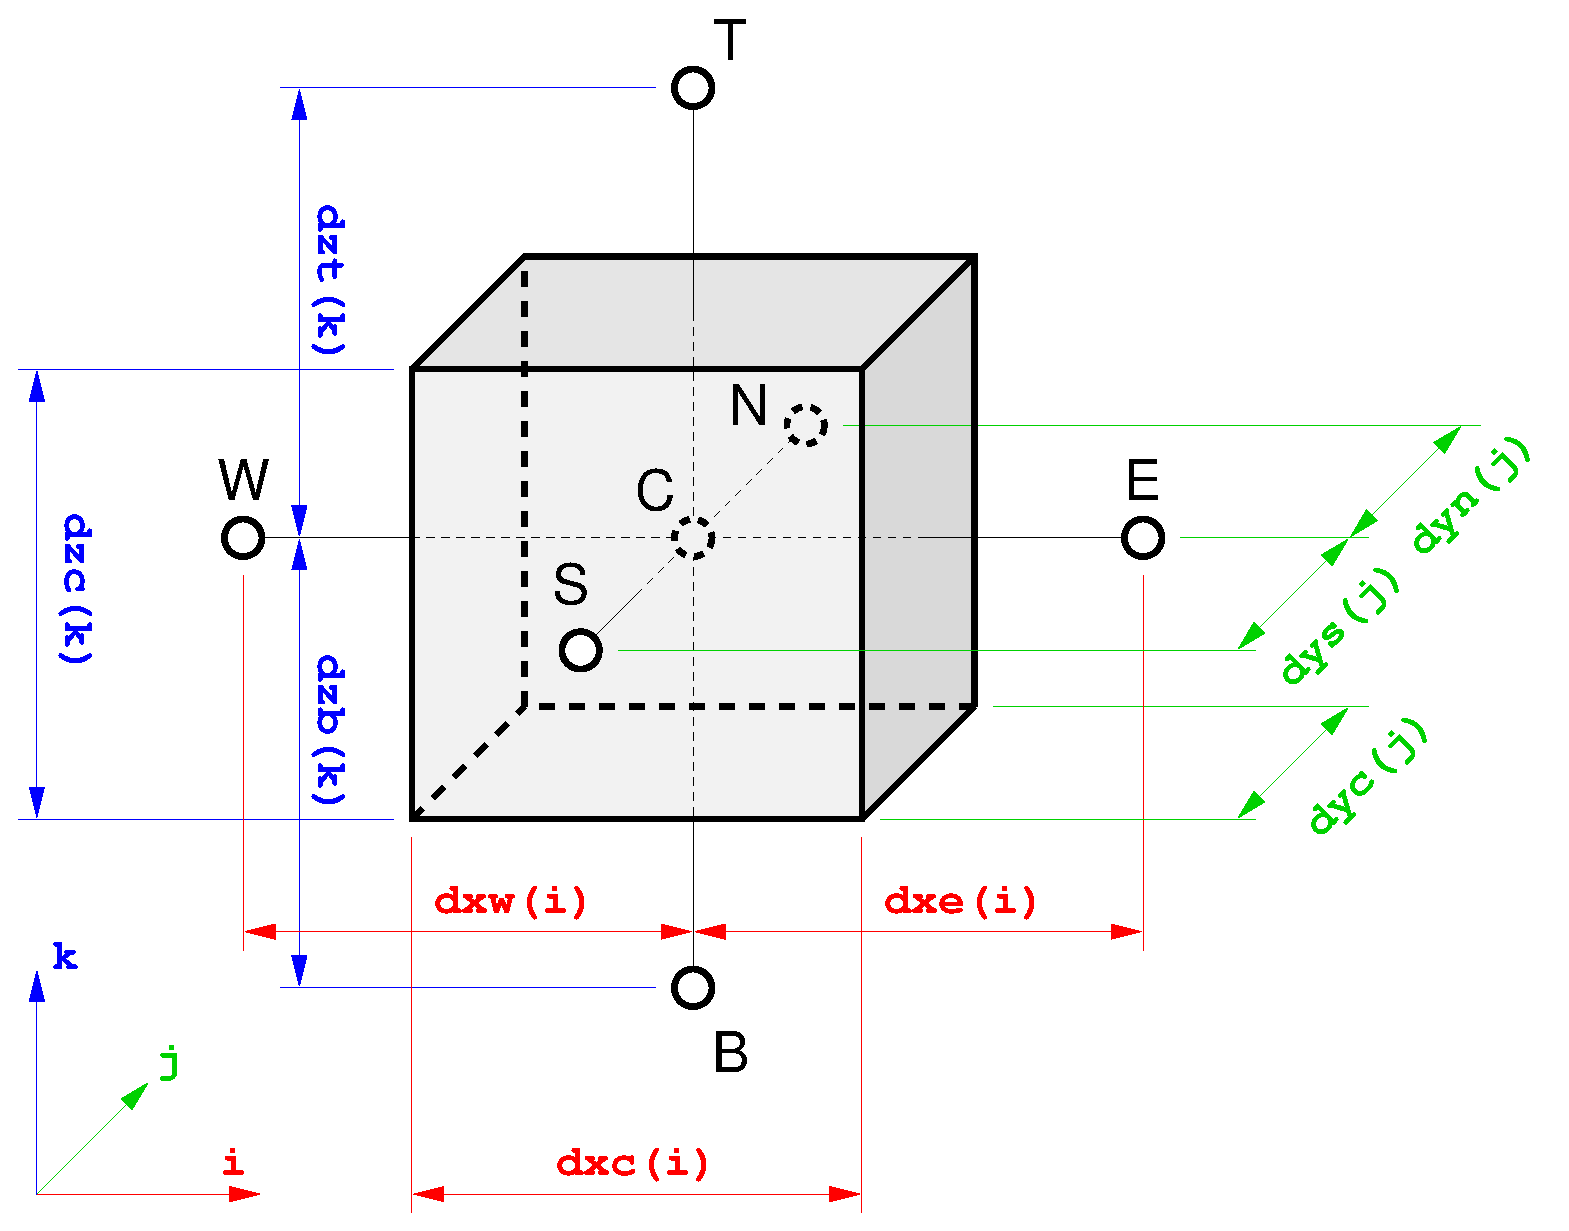
\includegraphics[scale=0.25]{Figures/09-02-cell-dimensions.eps}}
  \end{picture}
  \caption{Cell dimensions.}
  \label{fig_cell_dimensions}
\end{figure}

Lines~123--125 define constants to avoid {\em ghost numbers}. Line~126
just sends a message to the terminal. Loop spanning from line~127 
to~129 computes the $Nu$ and prints it to the terminal, together 
with $z$~coordinate. Here {\tt t[iw][j][k]}  is temperature at the
wall, {\tt t[ii][j][k]} is the temperature in the first computational
cell inside the domain, and {\tt t.dxw(ii)} is the distance between
the cell centre at~$i$ to the cell centre at~$i-1$, which is in {em this
case} at the wall. Distance {\tt dxw(i)} as well as other dimensions
for a general cell (not the one at the wall) are illustrated 
in~Fig.~\ref{fig_cell_dimensions}. 
%
Nusselt number for the heated wall ($x=-0.5$) is plotted in~Fig.~\ref{fig_nusselt}

%------------------%
%                  %
%  Nusselt number  %
%                  %
%------------------%
\begin{figure}[h!]
  \centering
  \setlength{\unitlength}{1mm}
  \begin{picture}( 70, 60)(0,0)
    \thickbox{ 70}{ 60}
    \put( 0, 0){\includegraphics[scale=0.35]{Figures/09-02-nusselt.eps}}
  \end{picture}
  \caption{Non-dimensional $u$~velocity distribution along the line~$x=0$ (left)
           and $w$~velocity distribution along the line~$z=0$.}
  \label{fig_nusselt}
\end{figure}

% \vspace{-20mm}
% \clearpage

%---------------------------------------------------------------------nutshell-%
\vspace*{5mm} \fbox{ \begin{minipage}[c] {0.97\textwidth} %-----------nutshell-%
    {\sf Section \ref{sec_thermally} in a nutshell} \\  %-------------nutshell-%
    
      - If solving a two-dimensional problem with {\psiboil} specify one
      coordinate direction as {\em homogeneous} by making it very thin compared
      to the others and by specifying periodic boundary conditions for it. \\
 
      - Minimum resolution in {\psiboil} is four cells. \\
 
      - When specifying forces for {\tt Momentum} equations, integrate
       them over {\em staggered} volumes ({\tt Vector::dV(m,i,j,k)}). \\
 
      - You can use and additional call to {\tt Pressure::update\_rhs}
      after the projection of velocity, to check the mass conservation
      reduction level. \\
 
      - Extracting profiles from post-processing packages is strongly
      discouraged, since they extract {\em interpolated} solutions, not the
      {\em computed} ones. \\

      - Profiles which are really computed in {\psiboil} can be extracted
      with objects of class {\tt Rack}. \\
 
     - Usage of {\tt Rack} is the same as that of {\tt Location}, except that,
     instead of three coordinates, one sends two coordinates and one {\tt Range}
     to it's constructor. \\

      - You can access all relevant cell dimensions using {\tt Scalar}s member
      functions {\tt dxc}, {\tt dyc}, {\tt dzc}, {\tt dxw}, {\tt dxe},
      {\tt dys}, {\tt dyn}, {\tt dzb} and {\tt dzt}.
 
  \end{minipage} } %--------------------------------------------------nutshell-%
%---------------------------------------------------------------------nutshell-%

  \section{Flow around a cube matrix}
\label{sec_cube_matrix}

In this section a flow around the cube matrix is solved using Direct Numerical
Simulation (DNS). It is a DNS in sense that not sub-grid-scale (SGS) model is
used, rather in the sense that it resolves {\em all} scales of motion. 
Cube matrix is placed at the bottom of the plane channel. The flow is
assumed to be fully developed, so it only suffices to simulate one flow
segment (flow around one cube) with periodic boundary conditions applied in
stream-wise~($x$) and span-wise~($y$) direction. Problem domain is illustrated
in Fig.~\ref{fig_matrix_domain}. The dimensions of the problem domain are
as follows: $D=6 \, [cm]$, $H=5.1 \, [cm]$ and $h=1.5 \, [cm]$. Working
fluid is air, having density $\rho = 1.205 \, [kg/m^3]$ and kinematic
viscosity~$\nu = 1.511 \times 10^{-5}$.

%-------------------%
%                   %
%  Matrix of cubes  %
%                   %
%-------------------%
\begin{figure}[ht]
  \centering
  \setlength{\unitlength}{1mm}
  \begin{picture}( 66, 44)(0,0)
    \thickbox{ 66}{ 44}
    \put(0,0){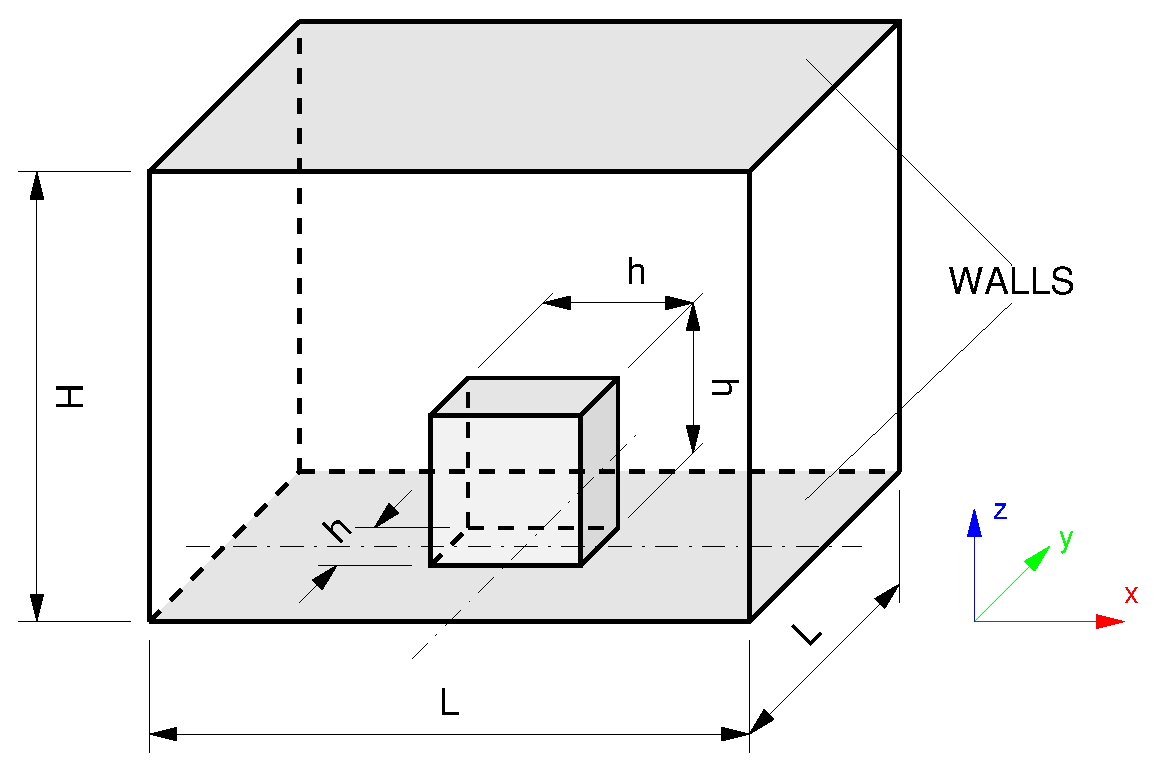
\includegraphics[scale=0.35]{Figures/09-03-matrix-gray.eps}}
  \end{picture}
  \caption{Problem domain for the flow around a cube matrix.} 
  \label{fig_matrix_domain}
\end{figure}

Flow rate for this case is specified with stream-wise bulk velocity equal 
to~$u_b = 3.86 \, [m/s]$. Reynolds number based on channel height 
is~$Re \approx 13000$. At this~$Re$, the flow is turbulent. This case,
in fact, is the first simulation of a turbulent flow in this tutorial.
{\psiboil} is a tool which simulates turbulent flows using Large Scale
Simulation (LSS) approaches, namely the DNS and LES\footnote{In more
general sense, LSS includes also simulation of turbulent flows with
interface tracking, but as it is still an active area of research,
nomenclature is not yet fully established.} 

Simulation of turbulent flows with LES/DNS consists of two steps:
%
\begin{itemize}
  \item Unsteady flow simulation
  \item Computation of flow statistics
\end{itemize}
%
First step generates a sequence of unsteady flow realizations stored on
a disk, while the second step reads the flow realizations from disk and
computes necessary statistics (Reynolds stresses, turbulent kinetic
energy, correlation, turbulent spectra, etc.). Having {\psiboil}'s
philosophy in mind\footnote{It is not an integral package suited for 
all flow situations one can encounter, but rather a suite of objects which 
facilitates building of different algorithms for flow simulation.} two
different programs will be outlined in this section: one for
unsteady flow simulation {\tt 09-03-main.cpp} and the other for
computation of flow statistics {\tt 09-03-stat.cpp}. Obviously these
two codes share some object definitions. The shared objects are stored
in {\tt C++} header file {\tt 09-03-common.h}.

\subsection{Unsteady flow simulation}
\label{sub_sec_unsteady_flow}

The program which conducts the unsteady flow simulation is very similar
to program introduced in~Sec.~\ref{sec_cylinder}. It also follows 
closely the typical {\psiboil} program layout introduced in Chap.~\ref{chap_structure}.

To compile it, you do not only need a link to {\em main} program in
{\em source} directory ({\tt PSI-Boil/Src}), but also to the include 
file~({\tt 09-03-common.h}). You can get the main program and the include 
file, provided you are in source directory, with:
%
\begin{verbatim}
> ln -i -s ../Doc/Tutorial/Volume1/Src/09-03-main.cpp main.cpp
> ln -i -s ../Doc/Tutorial/Volume1/Src/09-03-common.h .
\end{verbatim} 
%
The include file holds grids and domain definition, and is included in the 
main program with the:
%
{\small \begin{verbatim}
     13   #include "09-03-common.h"
\end{verbatim}}
%
There is nothing new in these definitions, so there is no need to
explain them in more detail here. {\tt Times} object is defined in
line:
%
{\small \begin{verbatim}
     16   Times time(100000, 0.00002); /* ndt, dt */
\end{verbatim}}
%
For an LSS, we do not expect to get a steady solution to the problem.
We are aware (and hopeful) that simulation will yield an unsteady
solution and we want to perform enough time steps to get a relevant
statistical sample for later computation of flow statistics. Here 
we set the number of time step to~$100000$. Time step which gives 
the~CFL number in the stable range~($0.3-0.4$) is $0.00002$. The
physical time of this simulation is thus $2 \, [s]$.

The program defines variables (velocity, pressure and their sources)
in lines~21--22. Boundary conditions for variables are set in lines~24--38.
That is followed by the definition of materials (lines~43--45),
solver (line~47), transport equations (lines~52 and~53). As usually,
multigrid solver is defined for pressure equation (in line~59).
For this case, the flow is not initialized, but the forces in momentum
equations are (lines~61 and~62). 

The time loop, which spans from lines~67--105, has all the steps
introduced before, say in~Sec.~\ref{sec_cylinder}, but it has a
small section which re-computes the pressure drop at each time 
step to keep the bulk velocity constant, and a section which 
periodically saves the data for later computations of flow
statistics.

Mass flow in computational domain is kept constant using the second
Newton's law:
%
\be
  F = m \cdot a \; \; \; \; [N]
\ee
%
If applied to a computational domain, acceleration $a$ is the rate
of change of bulk velocity. Force~$F$, on the other hand is integrated
pressure drop in the domain. Hence, second Newton's law, can be
written as:
%
\be
  \frac{\p p^n}{\p x} V 
  =
  m \cdot \frac{u_b^n - u_b^{n-1}}{\Delta t} \; \; \; \; [N]
\ee
%
We want the bulk velocity at new time step~($u_b^n$) to be equal to
the prescribed (desired) bulk velocity~($u_{des}$). Furthermore,
acknowledging that mass~$m$ divided by volume~$V$ is density, the
expression for pressure drop which gives the desired bulk velocity
in the new time step is:
%
\be
  \frac{\p p^n}{\p x} 
  = 
  \rho \cdot \frac{u_{des} - u_b^{n-1}}{\Delta t} 
  \label{eq_newton_second}
\ee
%
The implementation of this expression is given in lines~91--96.
%
{\small \begin{verbatim}
     91     real b_new = ns.bulk(Comp::u(), LX*0.333);
     92
     93     real p_drop = fluid.rho() * (b_des - b_new) / time.dt();
     94
     95     Comp m = Comp::u();
     96     for_vmijk(xyz,m,i,j,k) xyz[m][i][j][k] = p_drop * uvw.dV(m,i,j,k);
\end{verbatim}}
%
Line~91 computes bulk velocity in~$x$ direction using {\tt Momentum}'s
member function {\tt bulk}. As the parameter, this function takes the
desired component ({\tt Comp}) and the~$x$ coordinate at which the bulk 
velocity is computed\footnote{Although
it should be the same at any position.}. Line~93 is the implementation
of~Eq.~\ref{eq_newton_second}, while lines~95 and~96 insert new pressure
drop to the momentum equation.

Periodic savings of turbulent velocity fields are performed in line:
%
{\small \begin{verbatim}
    102     if( time.current_step() % 50 == 0 ) uvw.save("uvw", time.current_step());
\end{verbatim}}
%
The line~102 checks the reminder of division of the current time step
with~50, and if it is zero, velocity is saved in the binary
format, using the {\tt Vector}'s member function {\tt save}. This
member function is available for {\tt Scalar}s as well. The {\tt save}
functions just dumps the memory occupied by a certain field variable
into a binary file. As such, it can not be visualized with a post-processing
tool. The {\tt save} command saves the files with extension~{\tt .bck} 
(to remind of {\em backup}).
As with other {\psiboil} output function, even here each processors
writes it's own file but they can {\em not} be connected into a single
one using the {\tt Connect} program.

Lines~103 and~104:
%
{\small \begin{verbatim}
    103     if( time.current_step() % 5000 == 0) /* 5000 */
    104       boil::plot->plot(uvw,p,"uvw,p", time.current_step());
\end{verbatim}}
%
store variables (velocity and pressure) for post-processing each
5000 time steps. Examples of these unsteady flow fields (realizations)
are given in~Fig.~\ref{fig_matrix_velocity}.

%------------%
%            %
%  Velocity  %
%            %
%------------%
\begin{figure}
  \centering
  \setlength{\unitlength}{1mm}
  \begin{picture}(145,195)(0,0)
    \thickbox{145}{195}
    \put( -3,153){\includegraphics[width=4.8cm]{Figures/09-03/plane_xy_20000.eps}}
    \put( -3,103){\includegraphics[width=4.8cm]{Figures/09-03/plane_xz_20000.eps}}
    \put(  0,150){$z=7.5 \, [mm]$,  $t=0.4 \, [s]$}
    \put(  0,103){$y=30  \, [mm] $, $t=0.4 \, [s]$}

    \put( 47,153){\includegraphics[width=4.8cm]{Figures/09-03/plane_xy_40000.eps}}
    \put( 47,103){\includegraphics[width=4.8cm]{Figures/09-03/plane_xz_40000.eps}}
    \put( 50,150){$z=7.5 \, [mm]$,  $t=0.8 \, [s]$}
    \put( 50,103){$y=30  \, [mm] $, $t=0.8 \, [s]$}

    \put( 97,153){\includegraphics[width=4.8cm]{Figures/09-03/plane_xy_60000.eps}}
    \put( 97,103){\includegraphics[width=4.8cm]{Figures/09-03/plane_xz_60000.eps}}
    \put(100,150){$z=7.5 \, [mm]$,  $t=1.2 \, [s]$}
    \put(100,103){$y=30  \, [mm] $, $t=1.2 \, [s]$}

    \put( -3, 53){\includegraphics[width=4.8cm]{Figures/09-03/plane_xy_80000.eps}}
    \put( -3,  3){\includegraphics[width=4.8cm]{Figures/09-03/plane_xz_80000.eps}}
    \put(  0, 50){$z=7.5 \, [mm]$,  $t=1.6 \, [s]$}
    \put(  0,  3){$y=30  \, [mm] $, $t=1.6 \, [s]$}

    \put( 47, 53){\includegraphics[width=4.8cm]{Figures/09-03/plane_xy_100000.eps}}
    \put( 47,  3){\includegraphics[width=4.8cm]{Figures/09-03/plane_xz_100000.eps}}
    \put( 50, 50){$z=7.5 \, [mm]$,  $t=2 \, [s]$}
    \put( 50,  3){$y=30  \, [mm] $, $t=2 \, [s]$}

    \put( 97, 53){\includegraphics[width=4.8cm]{Figures/09-03/plane_xy_mirror_100000.eps}}
    \put( 97,  3){\includegraphics[width=4.8cm]{Figures/09-03/plane_xz_mirror_100000.eps}}
    \put(100, 50){$z=7.5 \, [mm]$,  time averaged}
    \put(100,  3){$y=30  \, [mm] $, time averaged}
  \end{picture}
  \caption{Unsteady and time-averaged velocity fields colored by the magnitude of 
           stream-wise~($x$) velocity component.}
  \label{fig_matrix_velocity}
\end{figure}

\subsection{Computation of flow statistics}
\label{sub_sec_flow_statistics}

Program for computation of flow statistics~({\tt 09-03-stat.cpp}) does not
follow the typical {\psiboil}'s program structure. Therefore, it is given
and explained here in full detail. 
%
{\small \begin{verbatim}
      1 #include "Include/psi-boil.h"
      2
      3 #include <vector>
      4
      5 /****************************************************************************/
      6 main(int argc, char * argv[]) {
      7
      8   boil::timer.start();
      9
     10   /*------------------------------+
     11   |  grids, obstacles and domain  |
     12   +------------------------------*/
     13   #include "09-03-common.h"
     14
     15   /*------------------+
     16   |  define unknowns  |
     17   +------------------*/
     18   Vector uvw(d);   // velocity
     19   Scalar ut(d);  Scalar vt(d);  Scalar wt(d);     // temporary u, v, w
     20   Scalar u (d);  Scalar v (d);  Scalar w (d);     // averaged  u, v, w
     21   Scalar uu(d);  Scalar vv(d);  Scalar ww(d);     // averaged  uu,vv,ww
     22   Scalar uv(d);  Scalar uw(d);  Scalar vw(d);     // averaged  uv,uw,vw
     23
     24   u  = 0; v  = 0; w  = 0;
     25   uu = 0; vv = 0; ww = 0;
     26   uv = 0; uw = 0; vw = 0;
     27
     28   /* timer */
     29   Times time(80000, 0.00002); /* ndt, dt */
     30   time.first_step(20000);
     31
     32   /*------------+
     33   |  time loop  |
     34   +------------*/
     35   real count = 0;
     36
     37   const Comp U = Comp::u();
     38   const Comp V = Comp::v();
     39   const Comp W = Comp::w();
     40
     41   for(time.start(); time.end(); time.increase()) {
     42
     43     /*-------+
     44     |  load  |
     45     +-------*/
     46     if( time.current_step() % 100 == 0 ) {
     47       boil::oout << "##########################" << boil::endl;
     48       boil::oout << "# GETTING TIME STEP: " << time.current_step() << boil::endl;
     49       boil::oout << "#-------------------------" << boil::endl;
     50
     51       count ++;
     52
     53       uvw.load("uvw", time.current_step());
     54
     55       for_vijk(u,i,j,k) {
     56         ut[i][j][k] = 0.5 * (uvw[U][i][j][k] + uvw[U][i+1][j]  [k]  );
     57         vt[i][j][k] = 0.5 * (uvw[V][i][j][k] + uvw[V][i]  [j+1][k]  );
     58         wt[i][j][k] = 0.5 * (uvw[W][i][j][k] + uvw[W][i]  [j]  [k+1]);
     59       }
     60
     61       u  += ut;     v  += vt;     w  += wt;
     62       uu += ut*ut;  vv += vt*vt;  ww += wt*wt;
     63       uv += ut*vt;  uw += ut*wt;  vw += vt*wt;
     64     }
     65   }
     66
     67   u  /= count;  v  /= count;  w  /= count;
     68   uu /= count;  vv /= count;  ww /= count;
     69   uv /= count;  uw /= count;  vw /= count;
     70
     71   uu -= u*u;  vv -= v*v;  ww -= w*w;
     72   uv -= u*v;  uv -= u*v;  vw -= v*w;
     73
     74   /*-------+
     75   |  plot  |
     76   +-------*/
     77   boil::plot->plot(u, v, w,   "velocity-mean", time.current_step()-1);
     78   boil::plot->plot(uu,vv,ww,  "stresses-mean", time.current_step()-1);
     79
     80   boil::timer.stop();
     81   boil::timer.report();
     82 }
\end{verbatim}}
%
This program includes the same file ({\tt 09-03-common.h}) as the program for 
unsteady flow simulation to ensure that grids and domains are the same. Fields
for unknowns are defined in lines~18--22. The {\tt Vector uvw} is defined
to loading the results generated in previous step, and~12 more scalars which 
follow will hold temporary (unsteady) velocity components ({\tt ut}, {\tt vt}, {\tt wt}),
time-averaged velocity components ({\tt u}, {\tt v}, {\tt w}) and Reynolds
stress components ({\tt uu}, {\tt vv}, \dots {\tt vw}). The {\tt Scalar}
field which are used for accumulating statistics are initialized in lines~24--26.

Line~29 defines the {\tt Timer}, but contrary to the previous program, it
will execute {\em only} 80000 time steps. However, the time stepping does
not start from zero, but from time step~20000, stipulated in line~30. By
doing so, we will discard first 20000 time steps (corresponding to $0.4 \, [s]$
physical time), thus gather statistics from the time when the flow is already 
fully developed\footnote{Actually, a much more concise procedure would be
needed to ensure this, but it is beyond the scope of this tutorial.}. 

{\tt real} variable~{\tt count} is defined and initialized in line~35. It stores
the number of samples (flow field realizations) used in the computation of
statistics. 

Time loop starts at line~41. This loop increases the counter in line~51 
and then reads the results performed in previous
simulation (program {\tt 09-03-main.cpp}) in line~53. {\tt Vector}'s member
function~{\tt load} is used to read the results and it does exactly the opposite
from {\tt save}: it reads the binary data stored in the {\tt .bck} file and
loads it directly into variable's memory space. This line will work properly 
only if the program is executed {\em on the same number of processors} as the 
simulation program was. 

Once the {\tt Velocity} field is loaded into {\tt uvw} field variable, it is
interpolated into three {\tt Scalar} fields in lines~55--59. {\tt Scalar} 
fields {\tt u}, {\tt v} and {\tt w} hold the unsteady velocity field components,
which are added into mean ones in line~61, and to variables which will hold
Reynolds stresses in lines~62 and~63. For the mean velocity components, simple 
addition is performed, while for the Reynolds stress variables appropriate 
multiplications are added. When the time loop ends (after line~65) these values 
are normalized by the number of samples~(lines~67--69) and Reynolds stresses are
finally computed in lines~71 and~72. 

The procedure for computation of Reynolds stresses might need more explanation.
A Reynolds stress component ($\ol{u'u'}$, for instance), at specified 
position is defined as:
%
\be
  \ol{u'u'} = \frac{1}{T} \int_T u'(t) u'(t) dt
  \label{eq_rs_def}
\ee
%
where over-bar denotes time-averaged value, $T$ is the period of time averaging 
and $u'(t)$ is velocity fluctuation defined as: 
%
\be
  u'(t) = u(t) - \ol{u}
  \label{eq_u_fluct_def}
\ee
%
where $u(t)$ is the magnitude of velocity component at time~$t$, 
while~$\ol{u}$ is the time-averaged velocity component defined as:
%
\be
  \ol{u} = \frac{1}{T} \int_T u(t) dt
\ee
%
What we really compute in line~56, and what we finally have after line~59 
is actually:
%
\be
  \ol{uu} = \int_T u(t) u(t) dt
  \label{eq_UU_def}
\ee
%
The relation between $\ol{u'u'}$ (which we want) and $\ol{uu}$ 
(which we can compute from flow realizations) can be obtained if definition 
of~$u'(t)$ (Eq.~\ref{eq_u_fluct_def}) is introduced into~Eq.~\ref{eq_rs_def}:
%
\bea
  \ol{u'u'} 
  & = & \frac{1}{T} \int_T (u(t) - \ol{u})(u(t) - \ol{u}) dt \\ \nonumber
  & = & \underbrace{\frac{1}{T} \int_T u(t) u(t) dt}_{\ol{uu}} 
      - 2 \ol{u} \underbrace{\frac{1}{T} \int_T u(t) dt}_{=\ol{u}} 
      +  \ol{u} \, \ol{u} \underbrace{\frac{1}{T} \int_T dt}_{=1}  
\eea
% 
where we placed~$\ol{u}$ is placed in front of time integrals, because
it is constant in time by definition. So the final form of equation for
computing $\ol{u'u'}$ is:
%
\bea
  \ol{u'u'} = \ol{uu} - \ol{u} \, \ol{u}
\eea
% 
which is exactly what program line~71 does. 

Once all the statistics are computed, the program saves the time-averaged
velocities from line~77 and diagonal trace of the Reynolds stress tensor
from line~78. Time-averaged velocity fields are shown in bottom right
corner of~Fig.~\ref{fig_matrix_velocity} and diagonal trace components
of the Reynolds stress tensor in~Fig.~\ref{fig_matrix_stresses}. 

%------------%
%            %
%  Stresses  %
%            %
%------------%
\begin{figure}[h!]
  \centering
  \setlength{\unitlength}{1mm}
  \begin{picture}(145, 95)(0,0)
    \thickbox{145}{ 95}
    \put( -4, 50){\includegraphics[width=5.0cm]{Figures/09-03/uu_xy.eps}}
    \put( -4,  5){\includegraphics[width=5.0cm]{Figures/09-03/uu_xz.eps}}
    \put( 10,  0){$\ol{u'u'}$ contours}

    \put( 47, 50){\includegraphics[width=5.0cm]{Figures/09-03/vv_xy.eps}}
    \put( 47,  5){\includegraphics[width=5.0cm]{Figures/09-03/vv_xz.eps}}
    \put( 61,  0){$\ol{v'v'}$ contours}

    \put( 98, 50){\includegraphics[width=5.0cm]{Figures/09-03/ww_xy.eps}}
    \put( 98,  5){\includegraphics[width=5.0cm]{Figures/09-03/ww_xz.eps}}
    \put(112,  0){$\ol{w'w'}$ contours}
  \end{picture}
  \caption{Diagonal trace components of the Reynolds stresses tensor for the
           flow around the cube matrix. Top: contours in
           plane~$z=7.5 \, [mm]$; bottom: contours in plane~$y=30 \, [mm]$.}
  \label{fig_matrix_stresses}
\end{figure}

%---------------------------------------------------------------------nutshell-%
\vspace*{5mm} \fbox{ \begin{minipage}[c] {0.97\textwidth} %-----------nutshell-%
    {\sf Section \ref{sec_cube_matrix} in a nutshell} \\  %-------nutshell-%
   
      - Turbulent flows in {\psiboil} are simulated using LSS techniques: 
      DNS and LES. \\  

      - Simulation by LSS techniques consists of two steps: unsteady flow
      simulation and computation of statistics. \\

      - In {\psiboil} a separate program is written for each step. \\

      - It is a good idea to place objects shared by these two programs
      in a separate include ({\tt C++ header}) file. \\

      - Bulk velocity in a computational {\tt Domain} in $x$, $y$ or $z$ 
      direction is in {\psiboil} computed using {\tt Momentum}'s member 
      functions {\tt Momentum::bulk\_i(real)}, {\tt Momentum::bulk\_j(real)} 
      or {\tt Momentum::bulk\_k(real)}. \\

      - {\tt Scalar} and {\tt Vector} type objects have member functions
      {\tt save} and {\tt load} which write and read their values in
      binary format. These file have the extension~{\tt .bck}.

  \end{minipage} } %--------------------------------------------------nutshell-%
%---------------------------------------------------------------------nutshell-%


%  \chapter{Two-phase Flows}

  \printindex

\end{document}
